\RequirePackage{colortbl}
\documentclass[shortabstract, mgr, english]{iithesis}

\usepackage{xcolor}
\usepackage[utf8]{inputenc}
\usepackage{graphicx}
\usepackage{float}
\usepackage{listings}
\usepackage{caption}
\usepackage{subcaption}
\usepackage{amsmath}
\let\lll\relax
\usepackage{amssymb}
\usepackage{enumitem}
\usepackage{booktabs}
\usepackage{hyperref}
\usepackage{url}
\usepackage{array}
\usepackage{algorithm}
\usepackage{algpseudocode}
\usepackage{tabularx}
\usepackage{multirow}
\usepackage[numbers]{natbib}

\definecolor{codebg}{RGB}{248,248,248}
\definecolor{codeframe}{RGB}{220,220,220}
\definecolor{keyword}{RGB}{0,92,197}
\definecolor{comment}{RGB}{0,128,0}
\definecolor{string}{RGB}{163,21,21}

\lstset{
  basicstyle=\ttfamily\small,
  backgroundcolor=\color{codebg},
  frame=single,
  rulecolor=\color{codeframe},
  breaklines=true,
  columns=fullflexible,
  keywordstyle=\color{keyword}\bfseries,
  commentstyle=\color{comment}\itshape,
  stringstyle=\color{string},
  showstringspaces=false,
  captionpos=b,
}

% Personal handles.
% \newcommand{\DEBUG}[1]{}     % Hide all.
\newcommand{\DEBUG}[1]{{#1}} % Display all.
\usepackage[T1]{fontenc}% Polskie literki
\newcommand{\TODO}[1]{\DEBUG{\tt{\textcolor{red}{TODO}(}{#1}{)}}}
\newcommand{\KOT}[1]{\DEBUG{\tt{\textcolor{orange}{KOT}(}{#1}{)}}}
\newcommand{\kr}{\text{\textcolor{orange}{$\blacktriangleright$}}}
\newcommand{\kl}{\text{\textcolor{orange}{$\blacktriangleleft$}}}
\newcommand{\KOTOK}[0]{\DEBUG{\tt{\textcolor{green}{OK}}}}
% Mark text changes for reviewer (red text)
\newcommand{\changed}[1]{\textcolor{red}{#1}}

\graphicspath{{img/}}

\newcolumntype{C}[1]{>{\centering\arraybackslash}m{#1}}

\polishtitle    {\changed{PCG Arena: platforma do zaślepionego testowania A/B\fmlinebreak generatorów treści proceduralnych\fmlinebreak z optymalizacją preferencji}}
\englishtitle   {PCG Arena: A Platform for Blind A/B Testing\fmlinebreak of Procedural Content Generators\fmlinebreak with Direct Preference Optimization \KOT{Kinga, to dobry tytuł PL?}}

\polishabstract {
\KOT{todo -- przeczytać PL potem}
Ewaluacja generatorów treści proceduralnych (PCG) dla gier wideo stanowi istotne wyzwanie metodologiczne, ponieważ przyjemność gracza jest z natury subiektywna i trudna do zmierzenia za pomocą automatycznych metryk. Niniejsza praca przedstawia PCG Arenę --- platformę internetową do ślepego testowania A/B generatorów poziomów do gry Super Mario Bros poprzez dane o preferencjach graczy. Platforma umożliwia graczom rozgrywanie dwóch proceduralnie generowanych poziomów obok siebie w przeglądarce, głosowanie na preferowany poziom oraz opcjonalne tagowanie cech rozgrywki. Głosy są agregowane za pomocą systemu ratingowego Glicko-2, który zapewnia rankingi z przedziałami ufności.

Na podstawie zebranych danych przeprowadzono analizę eksploracyjną charakteryzującą ranking preferencji generatorów, statyczny zakres ekspresyjny poziomów, trajektorie rozgrywki, heterogeniczność anonimowych użytkowników oraz semantykę tagów. Wyniki pokazują, że platforma może służyć zarówno jako ranking generatorów, jak i narzędzie diagnostyczne ujawniające ich tryby porażki. Finalnie, praca przedstawia MarioDPO --- generator poziomów wytrenowany metodą Direct Preference Optimization, który osiąga wynik preferencji 0.832, zbliżony do oryginalnych poziomów Nintendo.
}

\englishabstract {
Evaluating procedural content generators (PCGs) for video games poses significant methodological challenges, as player enjoyment is inherently subjective and difficult to quantify through automated metrics alone. This thesis presents PCG Arena, a web-based platform designed for blind A/B testing of Super Mario Bros level generators through human preference data.
\KOT{gdzieś - może tutaj - zdanie, że Mario has been an important benchmark for a variety of PCG methods, from 2009 until today, albo cos innego ale we wstępie od razu dającego do zroumienia, że to nie jest losowa gierka wzięta bo tak}
\changed{Super Mario Bros has been used as a benchmark for PCG level generation research since the first Mario AI Competition in 2009, making it an ideal domain for systematic generator comparison.} The platform enables players to play two procedurally generated levels side-by-side in their browser, vote for their preferred level, and optionally tag gameplay characteristics. Votes are aggregated using the Glicko-2 rating system, providing uncertainty-aware rankings with confidence intervals.

Building on the collected data, we conduct an exploratory analysis that characterizes generator preference rankings, static expressive range, gameplay trajectory fingerprints, anonymous-user heterogeneity, and tag semantics. The analysis shows that PCG Arena functions not only as a leaderboard, but also as a diagnostic instrument for understanding why generators win or fail. Finally, we present MarioDPO, a level generator fine-tuned with Direct Preference Optimization that achieves a preference score of 0.832, approaching the hand-crafted original Nintendo baseline.
}

\author         {Antoni Czapski}
\advisor        {dr Jakub Kowalski}
\date          {March 2026}
\transcriptnum {317214}
\advisorgen    {dr. Jakub Kowalski}

\begin{document}

\chapter{Introduction}
\label{ch:introduction}


\section{Procedural Content Generation in Video Games}
\label{sec:intro-pcg}

Procedural Content Generation (PCG) refers to the algorithmic creation of game
content---levels, maps, characters, items, narratives---with limited or indirect \KOT{OK, ale nie zacytowanie https://www.pcgbook.com to zbrodnia w kontekscie tej pracy :P }
human input~\citep{togelius2011search, summerville2018pcgml}\changed{\citep{shaker2016pcgbook}}. PCG has a long
commercial history: \emph{Rogue}~(1980) and \emph{Elite}~(1984) used algorithmic
generation to overcome memory constraints, and modern titles such as
\emph{Minecraft}, \emph{No Man's Sky}, and \emph{Spelunky} rely on procedural
generation as a core design pillar\changed{, providing variety, replayability, and vast explorable worlds}. Academic interest in PCG has grown steadily
since the mid-2000s, producing a rich landscape of generation techniques spanning
constructive rules, evolutionary search, formal grammars, neural networks, and
reinforcement learning.

Among the many game domains studied, Super Mario Bros (SMB) \changed{has accumulated the largest body of comparative work in} \changed{PCG level generation research}. Its 2D tile-grid format provides a
rich yet tractable design space, its physics are well understood, and the
open-source Mario AI Framework~\citep{karakovskiy2012marioai} offers a
standardised environment for both automated and human evaluation.\KOT{w sumie mało obrazków - może screenik z Mario żeby ludzie widzieli jak nie wiedzą :P} Over 15 years
of research has produced dozens of Mario level generators spanning \changed{most} major
PCG paradigm---yet evaluating and comparing them remains an open challenge.

\begin{figure}[H]
\centering
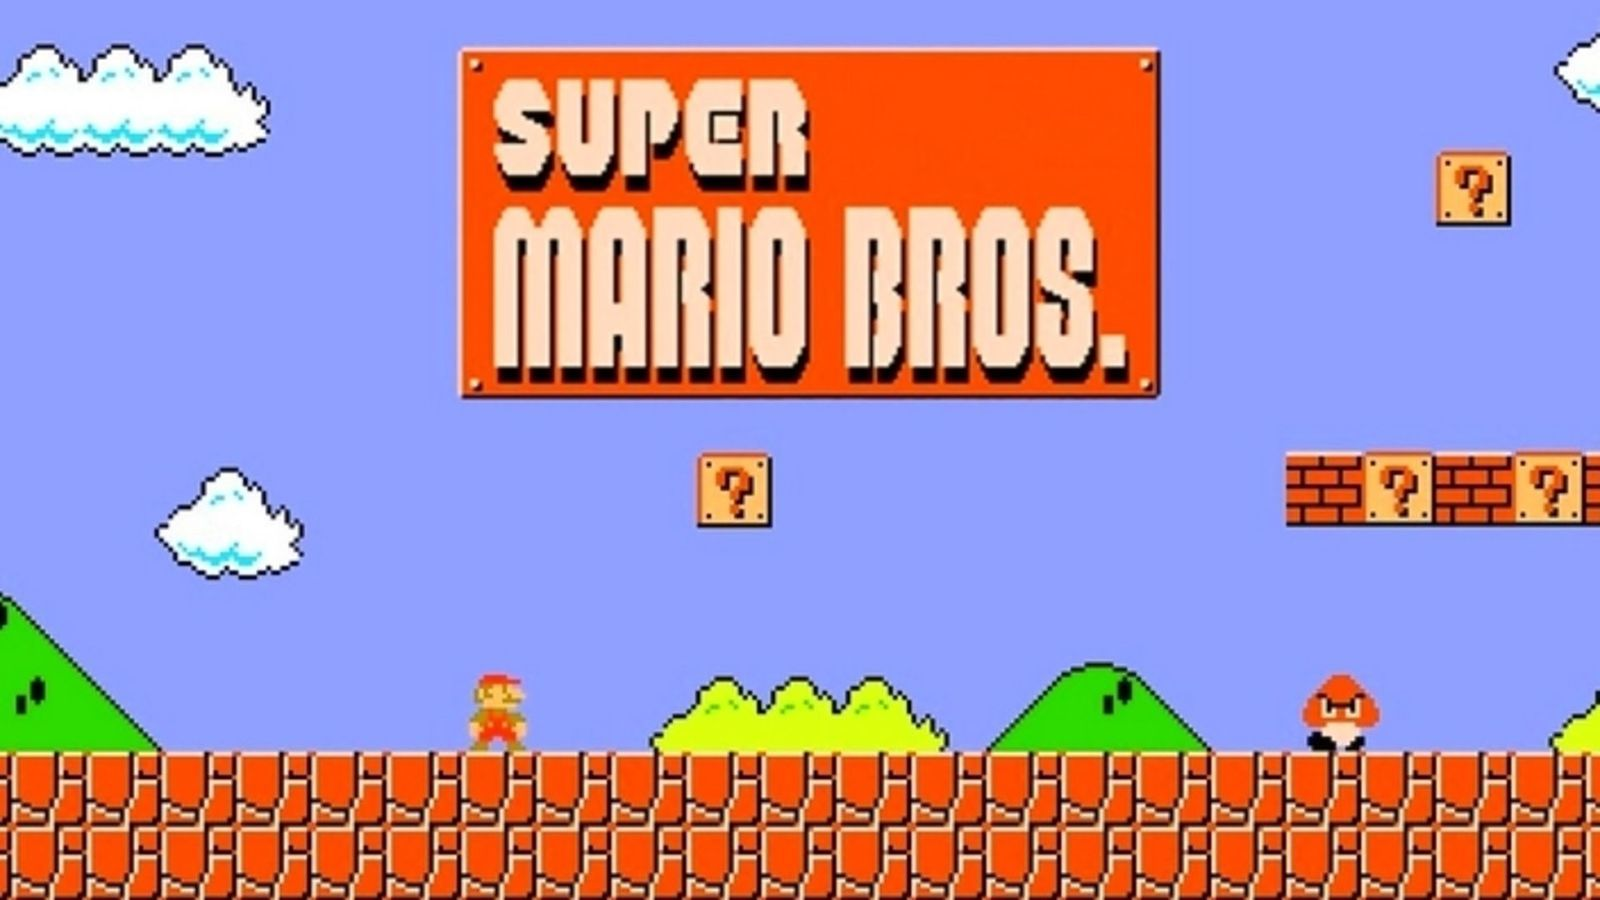
\includegraphics[width=0.75\textwidth]{smb-retro.jpg}
\caption{\changed{Screenshot of the original \emph{Super Mario Bros} (Nintendo, 1985). The player controls Mario through side-scrolling levels featuring platforms, enemies, power-ups, and coins. The 2D tile-grid structure of these levels provides the design space studied throughout this thesis.}}
\label{fig:smb-screenshot}
\end{figure}

\section{The Evaluation Problem}
\label{sec:intro-evaluation-problem}

Evaluating procedural content generators is fundamentally difficult because the
ultimate quality criterion---player enjoyment---is subjective, multidimensional,
and expensive to measure. The PCG literature has developed three families of
evaluation methods, each with significant limitations.

\textbf{Automated structural metrics}, such as linearity, leniency, and density,
can be computed directly from level tilemaps and are widely used for
characterising generator output~\citep{smith2010analyzing, horn2014comparative}.
However, \citet{marino2015empirical} demonstrated that these metrics only weakly
correlate with human-rated difficulty and enjoyment, concluding that ``current
computational metrics should not be used in lieu of user studies.'' Multiple
incompatible definitions of the same metric---at least three formulations of
leniency exist in the literature---further complicate cross-study comparisons.

\textbf{Agent-based testing} uses AI controllers---typically the A* agent from
the 2009 Mario AI Championship---as player proxies. Agent-derived features such
as jump count or completion fraction provide scalable difficulty
estimates~\citep{volz2018evolving}, but superhuman agents can solve levels that
human players cannot. Difficulty estimates depend on the specific agent policy,
introducing a systematic bias that is rarely quantified.

\textbf{Human evaluation studies} remain the gold standard but are expensive and
typically small-scale: controlled lab studies use 15--37
participants~\citep{shaker2011mario, marino2015empirical}, while larger web-based
studies sacrifice experimental control~\citep{pedersen2010modeling}.
\changed{Small samples cannot control for varying levels of gaming experience,
diverse player expectations, or learning effects across successive trials.}
Critically,
\changed{all existing studies were conducted as one-time events---often years
apart---rather than as a persistent evaluation infrastructure, and the largest
web-based studies predate the wave of ML-based generators (GANs, LLMs, diffusion
models) that have since reshaped the field.} \changed{Many of these studies also reveal which algorithm produced each level to participants, even though, when players know the source generator, expectations contaminate their judgments.} \KOT{I suppose how the original Mario PCG competition worked? exactly as your study - play two levels choose best?}

This persistent gap between scalable-but-inaccurate automated metrics and
valid-but-expensive human studies motivates the work presented in this thesis.

\section{Research Questions and Contributions}
\label{sec:intro-rq}

This thesis addresses the PCG evaluation gap through the design, deployment, and
analysis of \emph{PCG Arena}, a web-based platform for blind A/B testing of
Mario level generators. We investigate five research questions:

\begin{description}[style=nextline]
      \item[RQ1: Human preference ranking] Which generators are preferred by
      players in blind pairwise comparisons?
      \item[RQ2: Static expressive range] How do generators differ structurally,
      and which static properties align with player preference?
      \item[RQ3: Gameplay footprint] What behavioral signatures appear in player
      trajectories for each generator?
      \item[RQ4: User heterogeneity] Are anonymous player preferences and play
      styles homogeneous, or do visible subgroups emerge?
      \item[RQ5: Tag semantics] What do optional tags reveal about why levels win
      or lose?
\end{description}

\KOT{probably noindent here to make it look better}

\noindent The thesis makes four contributions:

\begin{enumerate}
    \item \textbf{PCG Arena}, a persistent, open-access web platform for blind
          A/B testing of Super Mario Bros level generators, featuring
          browser-based gameplay, Glicko-2 uncertainty-aware rankings, and a
          novel matchmaking algorithm (AGIS).
    \item \textbf{A user study} analysing 1,000 exported pairwise votes from 77
          anonymous browser/player IDs across 14 research generators, with 1,968
          played side records, embedded gameplay trajectories, and subjective
          tags.
    \item \textbf{An exploratory analysis pipeline} connecting blind preference
          votes to static expressive-range metrics, trajectory fingerprints,
          anonymous-user preference maps, and qualitative tag-based failure-mode
          diagnostics.
    \item \textbf{MarioDPO}, a level generator fine-tuned with Direct Preference
          Optimisation on arena votes, achieving a preference score of 0.832 and
          approaching the hand-crafted Nintendo baseline.
\end{enumerate}

\section{Thesis Structure}
\label{sec:intro-structure}

The remainder of this thesis is organised as follows.
Chapter~\ref{ch:background} surveys background and related work on procedural
content generation \KOT{(in the context of Maio level generation?)} \changed{in the context of Mario level generation,} evaluation methodology,
rating systems, and preference learning. Chapter~\ref{ch:system-design} describes the design and implementation
of the PCG Arena platform. Chapter~\ref{ch:eda} presents the user study and an
exploratory data analysis addressing the five research questions.
Chapter~\ref{ch:mariodpo} details the development of the Judge Function and the
MarioDPO generator. Chapter~\ref{ch:conclusions} summarises contributions,
discusses limitations, and outlines future directions.


\chapter{Background and Related Work}
\label{ch:background}

\section{Super Mario Bros}
\label{sec:bg-smb}

\begingroup\color{red}
Super Mario Bros (SMB), released by Nintendo in 1985, is a side-scrolling platform
game in which the player controls Mario through a sequence of levels. Each level is
composed of a 2D tile grid, typically 16 tiles tall and 150--210 tiles wide, scrolling
horizontally from left to right. The game's design vocabulary includes several
categories of elements:

\begin{itemize}[nosep]
  \item \textbf{Terrain and platforms.} Solid ground blocks (\texttt{X}), brick blocks
        (\texttt{S}) that can be broken by hitting from below, pyramid blocks
        (\texttt{\#}), and jump-through platforms (\texttt{\%}) form the physical
        structure of each level.
  \item \textbf{Interactive blocks.} Question blocks may contain coins or power-ups:
        a Super Mushroom (which transforms Small Mario into Super Mario, allowing him
        to break bricks and survive one extra hit), a Fire Flower (enabling ranged
        attacks), or a 1-Up Mushroom (extra life). Invisible blocks provide hidden
        rewards.
  \item \textbf{Enemies.} Goombas are defeated by jumping on them; Koopa Troopas
        retract into their shells, which can then be kicked as projectiles; Spikies
        (Spinies) cannot be stomped; and Bullet Bills are fired from cannons. Winged
        variants of each enemy add vertical movement.
  \item \textbf{Collectibles.} Coins are scattered across levels as floating items or
        hidden inside blocks. Collecting 100 coins grants an extra life.
  \item \textbf{Pipes.} Decorative or functional vertical structures, some of which
        spawn Piranha Plant enemies.
  \item \textbf{Level boundaries.} Each level begins at a Mario spawn point
        (\texttt{M}) and ends at a flag pole (\texttt{F}).
\end{itemize}

The game's physics---gravity, inertia, jump arcs, and collision detection---are
deterministic and well-characterised. These properties make SMB an ideal benchmark
for PCG research: the tile-grid format provides a discrete, tractable design space;
the mix of terrain, enemies, and power-ups yields a combinatorially rich yet
well-understood design vocabulary; and the game's cultural familiarity means that
nearly all experimental subjects already understand the controls and goals
(Figure~\ref{fig:smb-screenshot}).
\endgroup

\section{Procedural Content Generation}
\label{sec:bg-pcg}

Procedural Content Generation (PCG) is the algorithmic creation of game content
with limited or indirect human input~\citep{togelius2011search}. \changed{Drawing on the
taxonomies presented by \citet{togelius2011search} and \citet{summerville2018pcgml},}
% AC: Złagodzone sformułowanie --- te 5 paradygmatów to nasza synteza
% na podstawie obu prac, nie bezpośredni cytat z nich. "Drawing on"
% zamiast "The most common taxonomy" lepiej oddaje, że to nasza
% interpretacja inspirowana tymi źródłami.
\changed{we distinguish five broad generation paradigms:}
\KOT{trche nie wiem jak z tych obu paperów można powiedzieć że jest takich 5 paradygmatów generacji... przejrzałem je teraz tylko żeby sobie przypomnieć ale mi się to tochę nie spina z tekstami źródłowymi}

\begin{description}[style=nextline, leftmargin=1.5em]
    \item[Constructive / Rule-based] Sequentially place content according to
    hand-authored rules or grammars. Fast and reliable, but limited in
    expressiveness.
    \item[Search-based (SBPCG)] Frame generation as optimisation over a fitness
    function, typically using evolutionary algorithms. Flexible but
    computationally expensive.
    \item[Grammar / Pattern-based] Use \KOT{of?} formal grammars, design patterns, or
    $n$-grams to encode structural idioms. Captures human design style but
    requires pattern libraries.
    \item[Machine Learning (PCGML)] Train neural networks on existing
    human-designed content. Data-driven and expressive, but may lack diversity
    or playability guarantees.
    \item[Reinforcement Learning (PCGRL)] Frame level design as a Markov
    Decision Process; train an agent to construct content. Unlike PCGML,
    requires no corpus of existing levels---only a reward function that
    encodes the desired content properties.
\end{description}

These paradigms are not mutually exclusive; many modern systems are hybrids. For
instance, MarioGAN~\citep{volz2018evolving} combines a learned GAN with CMA-ES
search in its latent space. A further useful distinction is between \emph{offline}
generation (content pre-computed before the game ships) and \emph{online}
generation (content created at runtime, potentially adapting to the player).
Online generation enables personalisation but imposes stricter time
budgets---a theme central to experience-driven
PCG~\citep{yannakakis2011experience}. A desirable property of any generator is
\changed{\emph{controllability}}: the ability to accept parameters describing desired
content features and produce content that complies.\KOT{czemu contrallability jest nagle boldem jak wczesniej online / offline było emphem?}

\subsection{Search-Based Approaches}
\label{subsec:bg-search}

Search-Based PCG (SBPCG) frames content generation as an optimisation
problem~\citep{togelius2011search}. A \emph{fitness function} encodes the desired
properties of the content (e.g., playability, target difficulty, aesthetic
criteria), and an evolutionary algorithm---typically a genetic algorithm or
CMA-ES---searches a space of candidate solutions to maximise it.

The approach is attractive because fitness functions provide explicit, modular
designer control: one can compose playability constraints, difficulty targets,
and diversity objectives into a single optimisation criterion. However, SBPCG has
two well-known limitations. First, each fitness evaluation may require an
expensive simulation (e.g., running an A* agent through a candidate level).
Second, designing good fitness functions is itself a difficult problem---one that
mirrors the evaluation challenge motivating this thesis.

The Mario AI Level Generation Competition~\citep{shaker2011mario} featured
several search-based entries. More recent work has applied CMA-ES to the latent
space of trained generative models~\citep{volz2018evolving}, effectively combining
search-based and ML-based paradigms.

\subsection{Grammar-Based and Rule-Based Approaches}
\label{subsec:bg-grammar}

Constructive generators build content sequentially according to hand-authored
rules, typically working left-to-right through a level. The Notch generator
shipped with \emph{Infinite Mario
Bros}~\citep{karakovskiy2012marioai} is the canonical example: it iterates
through section templates (straight, hill, tubes, gaps, cannons) with fixed
selection probabilities and basic playability checks. Constructive methods are
fast and guarantee structural validity, but their expressive range is narrow.

Grammar-based approaches extend this idea by encoding design rules in a formal
grammar. \citet{shaker2012evolving} used \textbf{Grammatical Evolution} (GE) to
map integer genotypes to level phenotypes via context-free grammar productions,
combining the interpretability of grammars with evolutionary search.
\citet{smith2010analyzing} introduced \textbf{Launchpad}, a rhythm-based
generator that maps player actions to level geometry via a design grammar. The
same paper introduced \textbf{Expressive Range Analysis} (ERA)---the practice of
generating a large sample of levels, computing structural metrics, and
visualising their joint distribution---which has become the dominant method for
characterising PCG generators.

\subsection{Machine Learning-Based Generation (PCGML)}
\label{subsec:bg-pcgml}

Machine learning approaches to PCG (PCGML) train neural networks on existing
content to learn implicit design knowledge~\citep{summerville2018pcgml}. Several
architectures have been applied to Mario level generation:

\textbf{Sequence models.} \citet{summerville2016super} trained a 3-layer LSTM to
generate levels column-by-column using a ``snaking'' tokenisation that preserves
vertical adjacency. Co-generating levels with A*-agent play traces achieved
97\% playability.

\textbf{Generative adversarial networks.} MarioGAN~\citep{volz2018evolving}
trains a Deep Convolutional GAN on sliding-window segments from a single
original SMB level. CMA-ES then searches the GAN's latent space to optimise
fitness functions based on tile distributions or agent-derived playability. This
work established the \textbf{Latent Variable Evolution} (LVE) paradigm.

\textbf{Large language models.} MarioGPT~\citep{sudhakaran2023mariogpt}
fine-tunes DistilGPT-2 on column-tokenised Mario levels with text-prompt
conditioning (e.g., ``many pipes, many enemies, low elevation''), enabling the
first natural-language-controllable level generator. 88\% of generated levels
are playable without post-processing.

\textbf{Diffusion models.} MarioDiffusion~\citep{schrum2025mariodiffusion} uses a
text-conditioned UNet denoiser to generate $16 \times 16$-tile scenes from
natural-language captions, representing the latest generation of multimodal PCG.

\textbf{Reinforcement learning.} PCGRL~\citep{khalifa2020pcgrl} formulates level
design as an MDP and trains an RL agent to edit tile grids, bypassing the need
for training data entirely.


\section{Super Mario Bros as a PCG Benchmark}
\label{sec:bg-mario}

\changed{Several practical factors explain why Super Mario Bros recurs throughout the
PCG literature.} Its 2D tile-grid format provides a rich yet tractable design space, its
physics introduce no new mechanics after the first level (isolating level design
as the sole variable of interest), nearly all experimental subjects are familiar
with the game's controls and goals, and the open-source Mario AI Framework
provides a standardised evaluation environment.

\subsection{The Mario AI Framework}
\label{subsec:bg-mario-framework}

The Mario AI Framework~\citep{karakovskiy2012marioai} is an open-source Java
implementation based on \emph{Infinite Mario Bros}, a public-domain clone of
Nintendo's Super Mario Bros created by Markus Persson in 2008. It served as the
basis for three tracks of the Mario AI Championship (2009--2012):

\begin{enumerate}[nosep]
    \item \textbf{Gameplay Track}---build a controller that plays levels as well
          as possible.
    \item \textbf{Learning Track}---build a controller that learns to play.
    \item \textbf{Level Generation Track}---build software that generates levels
          for human players.
\end{enumerate}

The Level Generation Track~\citep{shaker2011mario} was the first academic PCG
competition. Generators received gameplay metrics from a test level and had
60~seconds to produce a personalised level. Six entries competed; evaluation used
pairwise forced-choice (``which was more fun?'') with 15 human judges. This
competition established several norms that influenced subsequent research:
pairwise comparison as the preferred human evaluation protocol, player telemetry
as input to adaptive generators, and the A* agent as a \emph{de facto}
playability oracle.

Levels are stored as 2D character grids (ASCII tilemaps), where each character
encodes a functional tile type. The Video Game Level Corpus
(VGLC)~\citep{summerville2016super} standardised this encoding across all 32
original SMB levels and has been widely used as training data for neural
generators.

\subsection{Mario Level Generators in the Literature}
\label{subsec:bg-mario-generators}

The PCG Arena platform includes 15 generators spanning all major paradigm
families, selected to benchmark a broad cross-section of established PCG
approaches. Table~\ref{tab:generators} provides a comparative overview.

\KOT{gdzieś bym jeszcze wspomniał, nie wiem jakie miejsce jest dobre, że nie wszyscy potrafią generować to samo i że wiele z zaprezentowanych podejśc upraszcza sobie życie generując tylko 1-2 rodzaje przeciwników, albo tylko kilka rodzajów bloków. Swoja droga pytanie czy to nie jest issue że o samej grze i co składa się na level dowiadujemy się tak późno w pracy...}

\changed{An important caveat is that these generators do not all target the
same design vocabulary. Several reduce the problem space substantially---for
instance, restricting themselves to one or two enemy types (typically Goombas
and Green Koopas) or omitting power-ups, pipes carrying Piranha Plants, or
Bullet Bill cannons. This unevenness affects fair comparison: a generator
producing only a subset of SMB's design elements may appear competitive on
some metrics while being structurally less expressive than the original
Nintendo levels.}

\textbf{Human-authored baseline.} The 15 original SMB levels from Nintendo
(1985), transcribed into the Mario AI Framework's format. These serve as the
quality ceiling against which all algorithmic generators are measured.

\textbf{Constructive generators.} Four generators build levels left-to-right
using probabilistic placement: the \emph{Notch} generator shipped with Infinite
Mario Bros, its \emph{Parameterized} variant (NotchParam) exposing six tunable
difficulty/style knobs~\citep{shaker2011mario}, a \emph{Randomized} variant
(NotchParamRand) that randomly samples parameters per level, and \emph{Hopper},
which alternates generated and pre-designed segments with adaptive probability
adjustment.

\textbf{Chunk-based assembly.} \emph{Occupancy-Regulated Extension}
(ORE)~\citep{mawhorter2010occupancy} \KOT{tu i w kolejnych akapitach brakuje mi 'that' do spoójności przedstawiania co robią generatory względem wcześniejszego tekstu} \changed{is a method that} builds levels by iteratively attaching
hand-authored chunks at compatible anchor points, producing structurally
distinctive levels.

\textbf{Search-based generators.} The \emph{Grammatical Evolution} (GE)
generator~\citep{shaker2012evolving} evolves level-construction programs via a
context-free grammar. Three \emph{Pattern-based}
generators~\citep{dahlskog2014procedural} represent levels as sequences of
micro-patterns extracted from original SMB levels and use evolutionary search
with different fitness functions: pattern count (maximising motif frequency),
pattern occurrence (maximising motif diversity), and weighted pattern count
(rewarding rare motifs).

\textbf{Neural generators.} \emph{MarioGAN}~\citep{volz2018evolving} combines a
DCGAN with CMA-ES latent-space search.
\emph{MarioGPT}~\citep{sudhakaran2023mariogpt} uses a fine-tuned DistilGPT-2
with text-prompt control.
\emph{MarioDiffusion}~\citep{schrum2025mariodiffusion} generates tile scenes from
natural-language captions via a diffusion model. Finally, \emph{MarioDPO}---this
thesis's contribution---fine-tunes a GPT-2-based generator with Direct Preference
Optimisation using PCG Arena votes.

\begin{table}[H]
\centering
\footnotesize
\begin{tabular}{@{} l l l l r @{}}
\toprule
\textbf{Generator} & \textbf{Paradigm} & \textbf{Key technique} & \textbf{Control} & \textbf{Year} \\
\midrule
Original SMB1      & Human        & Manual design               & ---            & 1985 \\
Notch              & Constructive & Probabilistic L-to-R        & None           & 2008 \\
NotchParam         & Constructive & Probabilistic + 6 params    & Param.\ knobs  & 2011 \\
NotchParamRand     & Constructive & Probabilistic + random      & Random         & 2011 \\
Hopper             & Constructive & Adaptive probabilistic      & Adaptive       & 2010 \\
ORE                & Chunk-based  & Anchor-point assembly       & None           & 2010 \\
GE                 & Search       & Grammatical evolution       & Via grammar    & 2012 \\
Pattern Count      & Search       & Evolutionary (pattern freq.)& Fitness wts.   & 2014 \\
Pattern Occurrence & Search       & Evolutionary (unique patt.) & Fitness wts.   & 2014 \\
Pattern Wt.\ Count & Search       & Evolutionary (rarity-wt.)   & Fitness wts.   & 2014 \\
MarioGAN           & ML (GAN)     & DCGAN + CMA-ES latent       & Fitness fn.    & 2018 \\
MarioGPT           & ML (LLM)     & Fine-tuned DistilGPT-2      & Text prompts   & 2023 \\
MarioDiffusion     & ML (Diff.)   & Text-conditioned UNet       & Text captions  & 2025 \\
MarioDPO           & ML + DPO     & GPT-2 + pref.\ alignment    & Text + DPO     & 2026 \\
\bottomrule
\end{tabular}
\caption{Generators included in PCG Arena. All except MarioDPO (this thesis) are
previously published or reference implementations.}
\label{tab:generators}
\end{table}

By including generators from all paradigm families and spanning nearly four
decades of game content creation, PCG Arena tests whether human preference data
can discriminate generator quality more reliably than automated metrics.


\section{Evaluation Methods for Procedural Content}
\label{sec:bg-evaluation}

Evaluation is the central methodological challenge in PCG research and the
primary motivation for PCG Arena. This section surveys the main families of
evaluation methods used in the Mario PCG literature.

\subsection{Automated Metrics}
\label{subsec:bg-eval-automated}

The most widely used evaluation approach computes \emph{static structural
metrics} directly from the tile grid, without simulating gameplay.

\textbf{Linearity} measures how closely a level's vertical profile follows a
straight line. \citet{smith2010analyzing} defined it as the \changed{mean
absolute residual---the average vertical distance between platform midpoints
and the best-fit regression line---so that lower values indicate a more linear
level}. Later works~\citep{horn2014comparative,
summerville2017understanding} instead use $R^2$ \KOT{co to za wzorek, po co te literki i nazwy, to nic nie mowi, nic nie tłumaczy} \changed{(the coefficient of determination, measuring
the proportion of variance in the data explained by the regression),} \changed{which inverts the scale: higher $R^2$ means more linear. The two formulations are therefore not directly comparable, complicating cross-paper analyses.}

\textbf{Leniency} approximates difficulty through weighted sums of game objects.
\changed{In its original form~\citep{smith2010analyzing}, it is computed as
$L = (w_p \cdot n_p + w_g \cdot n_g + w_e \cdot n_e) / W$, where $n_p$ is the
number of power-ups, $n_g$ the number of gaps, $n_e$ the number of enemies, $W$
the level width in tiles, and the weights $w_p > 0$, $w_g, w_e < 0$ reward
forgiving content and penalise hazards.} At least three incompatible formulations exist in the literature, using different
tile weights and normalisation schemes~\citep{smith2010analyzing,
shaker2012evolving, marino2015empirical}. Critically,
\citet{marino2015empirical} showed that leniency only weakly correlates with
human-rated difficulty.

\textbf{Compression distance} (gzip-based Normalised Compression Distance)
quantifies structural similarity between level pairs and is used as a diversity
proxy~\citep{shaker2012evolving, horn2014comparative}.

\textbf{Expressive Range Analysis} (ERA), introduced by
\citet{smith2010analyzing}, generates a large sample of levels, computes two
metrics per level (classically linearity vs.\ leniency), and visualises the joint
distribution as a 2D histogram, revealing a generator's output peaks, holes, and
biases. ERA has been widely adopted~\citep{horn2014comparative,
shaker2012evolving} but is purely descriptive---it characterises \emph{what} a
generator produces, not whether players enjoy it.

\changed{Figure~\ref{fig:era-grid} shows an ERA grid for the 13 PCG Arena
generators, computed over 100 levels per generator (15 for the original SMB1
baseline). Each panel is a 2D histogram of linearity (using the $R^2$
formulation) against leniency. The plot reveals each generator's expressive
range: e.g.\ Notch and its variants concentrate near high-linearity, low-hazard
regions, while pattern-based and learned generators populate broader regions
of the design space.}

\begin{figure}[H]
\centering
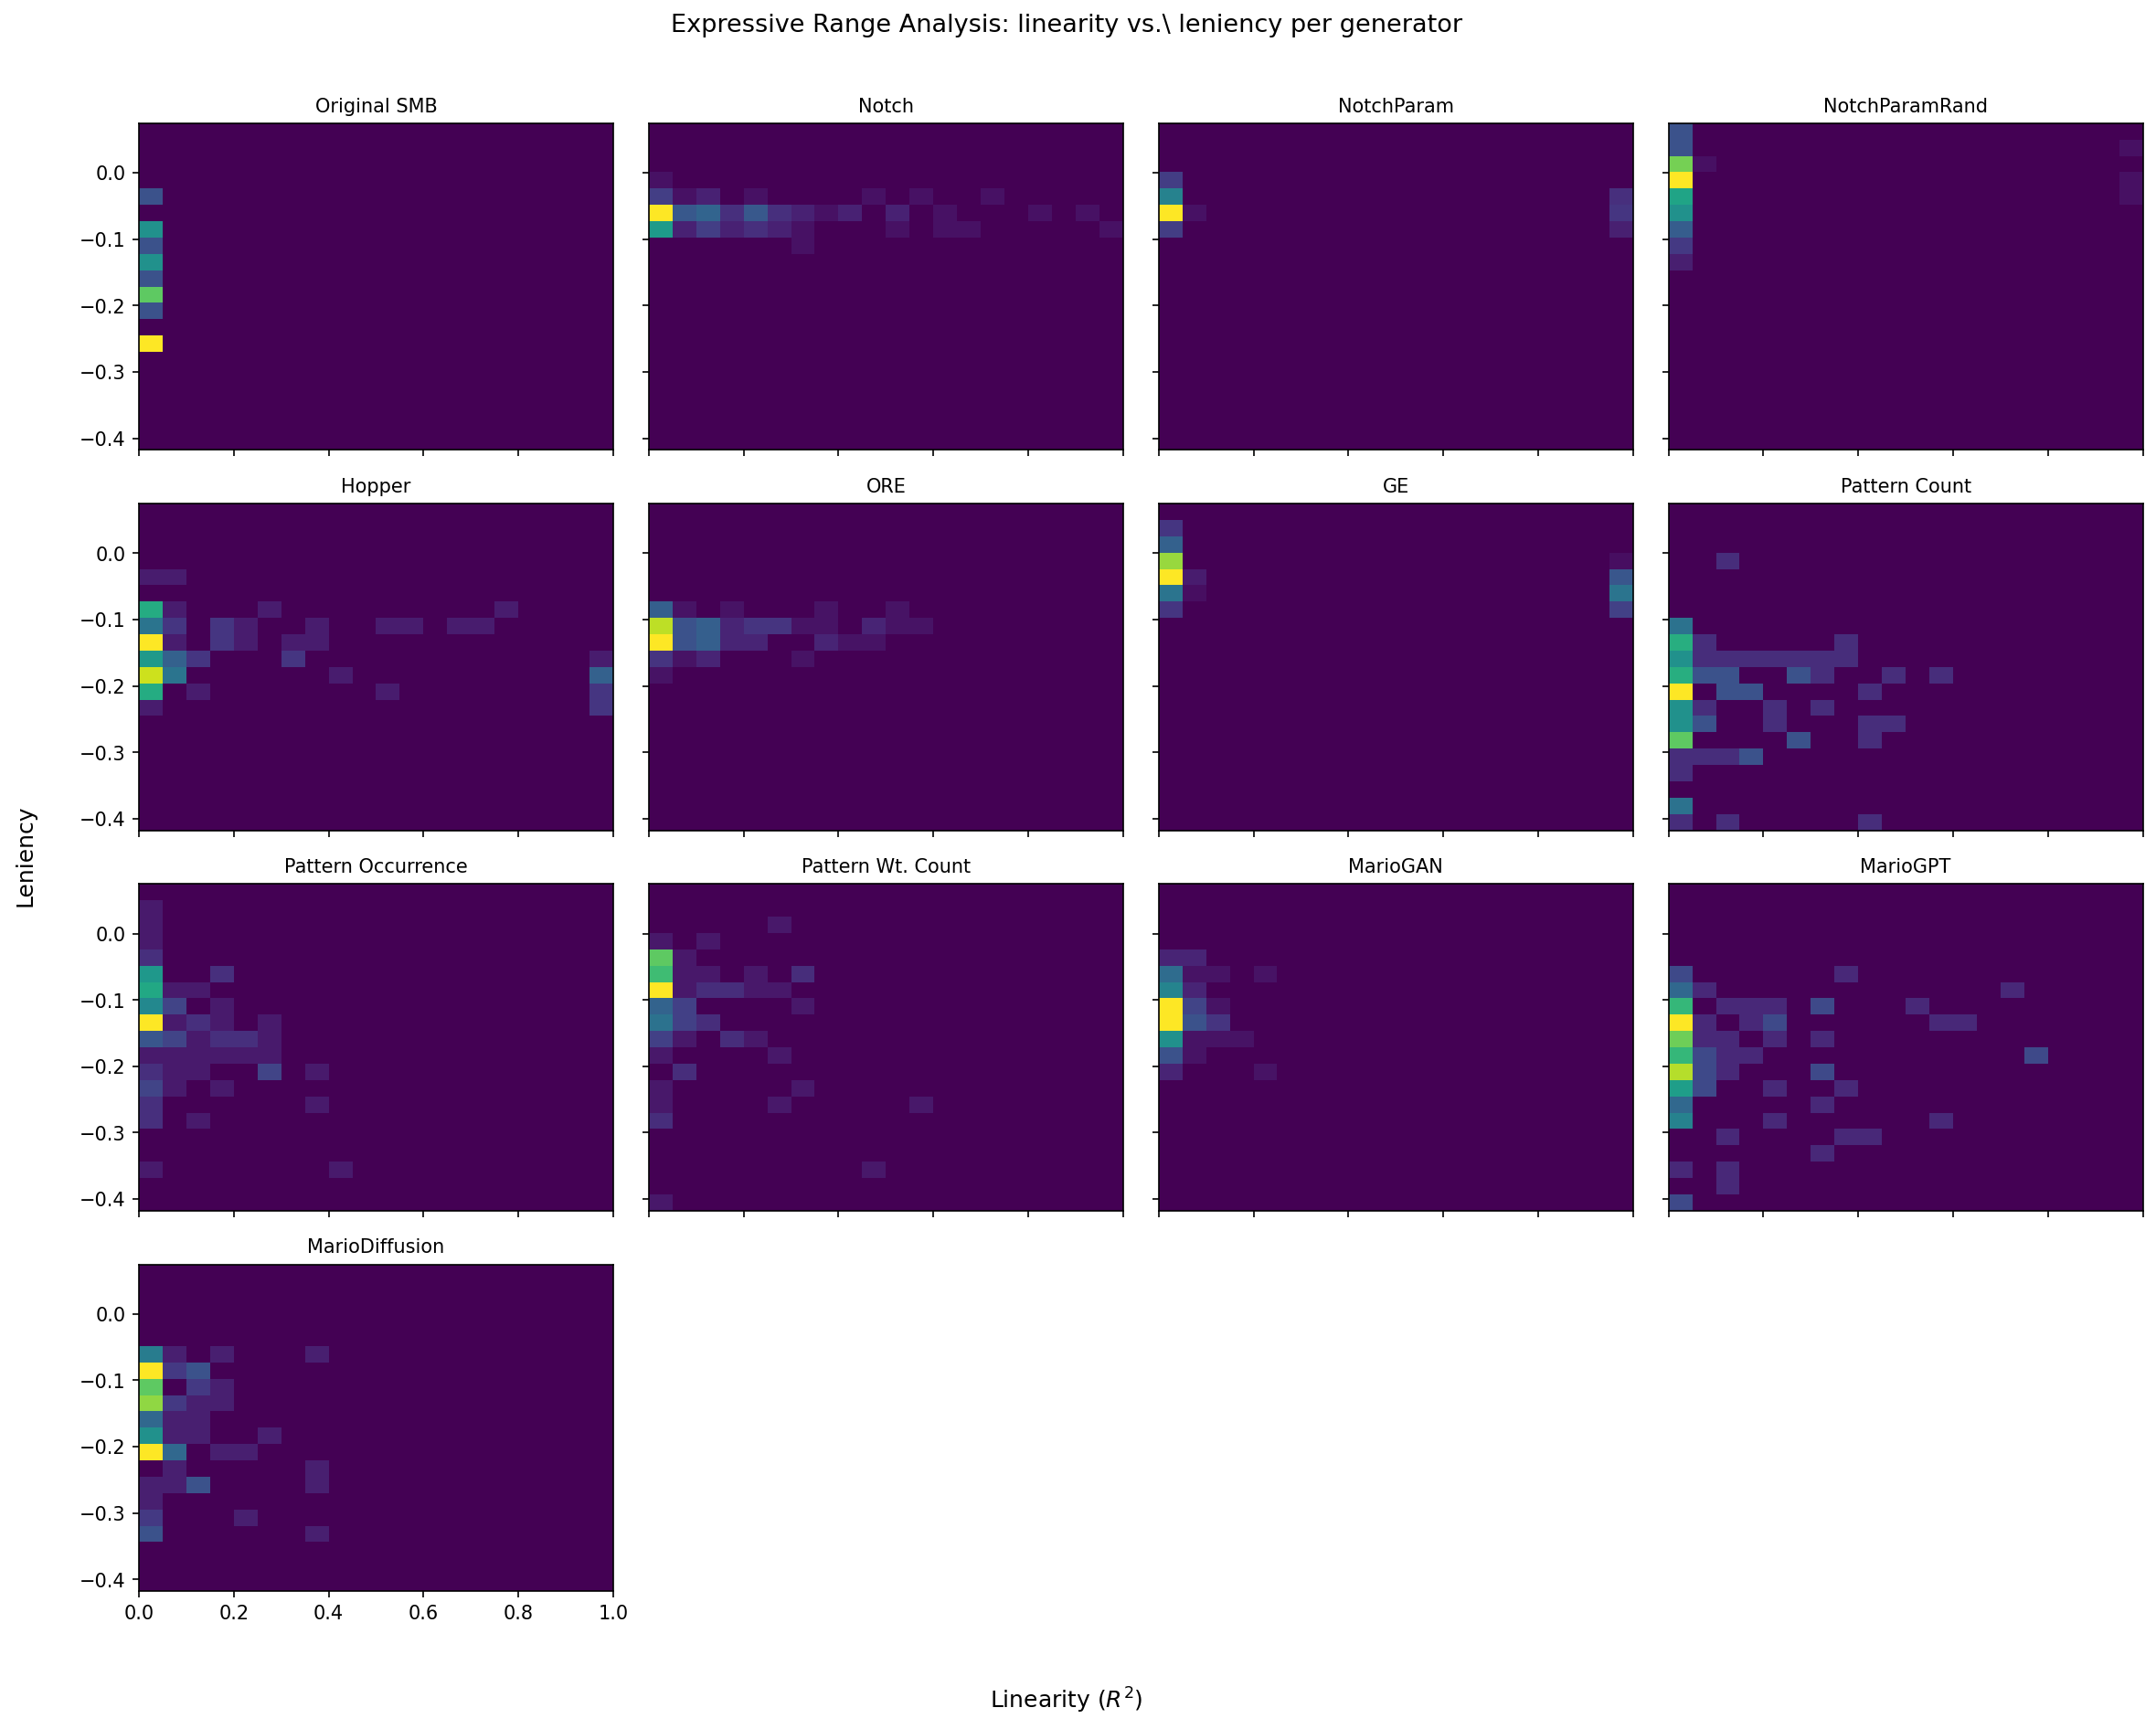
\includegraphics[width=\textwidth]{era-linearity-leniency.png}
\caption{\changed{Expressive Range Analysis grid: 2D histogram of linearity
($R^2$) versus leniency for each PCG Arena generator. Each panel uses the
same axes; brighter cells indicate more levels at that combination.}}
\label{fig:era-grid}
\end{figure}

\subsection{Agent-Based Testing}
\label{subsec:bg-eval-agents}

AI agents serving as player proxies enable scalable, repeatable assessment of
playability and difficulty.

\textbf{Playability gates.} A level is deemed playable if a strong A* agent can
complete it. This binary check is the most common first stage in PCG evaluation
pipelines~\citep{volz2018evolving, summerville2016super, khalifa2020pcgrl}.

\textbf{Difficulty proxies.} Agent-derived metrics include jump count (the
number of jumps the A* agent performs, interpreted as difficulty), completion
fraction (progress along the $x$-axis if the level is not fully completable),
and virtual damage from stochastic ``human-like'' agents that model input timing
inaccuracies~\citep{nam2024using}.

Agent-based evaluation is fast, reproducible, and incurs no participant cost, but
agent bias is a fundamental concern: superhuman agents can solve levels humans
cannot, and difficulty estimates depend on the specific agent policy. \changed{The mismatch also goes the other way:
many levels that human players can complete are unsolvable by standard A* agents,
which lack the ability to backtrack, use special power-ups, or exploit advanced
movement techniques. These bi-directional} limitations are rarely quantified in
the literature.
\KOT{czytam podobny tekst już 2 czy trzeci raz w tej pracy ten tekst i brakuje mi, tu lub wcześniej, przeciwwagi: że jest masa leweli przechodzalnych przez ludzi którzych te używane AI nie potrafią - głównie bo backtracking i special skille}

\subsection{Human Evaluation Studies}
\label{subsec:bg-eval-human}

Human studies remain the gold standard for PCG evaluation but vary widely in
scale and methodology.

\textbf{Pairwise forced-choice.} The Mario AI
Championship~\citep{shaker2011mario} asked 15 judges to play two levels and
select ``which was more fun?'' without further defining ``fun.'' This protocol
directly inspired PCG Arena's design.

\textbf{Likert-scale ratings.} \citet{marino2015empirical} used 7-point Likert
scales \changed{(ordered response scales from ``strongly disagree'' to ``strongly agree'')}
for enjoyment, aesthetics, and difficulty \changed{with $n = 37$ participants}.\KOT{wtf is n?}
\citet{summerville2017understanding} collected ratings across 85 design metrics
and showed that inter-rater agreement imposes ceilings on achievable
metric--human correlations. \changed{The practical consequence is a quantitative
upper bound: an automated metric cannot correlate with human ratings any better
than humans correlate with each other, so reporting an inter-rater agreement
baseline is essential when interpreting metric--human correlations---a
discipline rarely followed in the PCG literature.}
\KOT{also - what is likert scale...}

\textbf{Large-scale web studies.} \citet{pedersen2010modeling} collected
240~game pairs via a web deployment of \emph{Infinite Mario Bros} variants
for pairwise affective-preference analysis.
A follow-up by \citet{shaker2011features} collected 600
game-pair comparisons via an uncontrolled web applet, but the number of unique
participants is not reported.
Both studies date from 2010--2011 and predate the wave of ML-based generators
(GANs, LSTMs, diffusion models) that have since reshaped the field.

These studies collectively demonstrate that while \changed{human empirical} evaluation provides the
most valid quality signal, it is expensive, typically small-scale ($n < 40$ in
controlled settings), and \changed{conducted as isolated, one-time events rather
than within a persistent evaluation infrastructure}.
\changed{Earlier work on automatic personalised content
generation~\citep{shaker2010towards} and design-pattern
analysis~\citep{dahlskog2013patterns} further explored the relationship between
level structure and player preferences, but likewise relied on small participant
pools.}
Moreover, even the largest prior web study was conducted before modern
generative methods existed, leaving a significant gap in comparative human
evaluation of contemporary Mario level generators.

\KOT{więcej tego jeszcze było z human studies: https://ojs.aaai.org/index.php/AIIDE/article/view/12399/12258 oraz http://julian.togelius.com/Dahlskog2013Patterns.pdf  ze slajdów złapałem co mi się przypomniało}

\subsection{Comparison of Approaches and Their Limitations}
\label{subsec:bg-eval-comparison}

Table~\ref{tab:eval-comparison} summarises the evaluation methods employed across
key papers in the Mario PCG literature.

\begin{table}[H]
\centering
\small
\begin{tabular}{lllccccc}
\toprule
\textbf{Paper} & \textbf{Year} & \changed{\textbf{PCG algorithm}} & \textbf{S} & \textbf{A} & \textbf{ERA} & \textbf{H} & \textbf{ML} \\
\midrule
Smith \& Whitehead          & 2010 & \changed{Launchpad (rhythm-based)} & $\checkmark$ &              & $\checkmark$ &              &              \\
Pedersen et al.             & 2010 & \changed{Notch (parameterised)}   & $\checkmark$ &              &              & $\checkmark$ & $\checkmark$ \\
Shaker et al.\ (Champ.)     & 2011 & \changed{Comp.\ entries (mixed)}  & $\checkmark$ & $\checkmark$ &              & $\checkmark$ &              \\
Shaker et al.\ (GE)         & 2012 & \changed{Grammatical Evolution}   & $\checkmark$ &              & $\checkmark$ &              &              \\
Horn et al.                 & 2014 & \changed{Multiple (comparative)}  & $\checkmark$ &              & $\checkmark$ &              &              \\
Marino et al.               & 2015 & \changed{GE + Notch (compared)}   & $\checkmark$ &              &              & $\checkmark$ &              \\
Summerville \& Mateas       & 2016 & \changed{LSTM column generator}   & $\checkmark$ & $\checkmark$ &              &              & $\checkmark$ \\
Summerville et al.          & 2017 & \changed{Multiple (8 generators)} & $\checkmark$ & $\checkmark$ &              & $\checkmark$ & $\checkmark$ \\
Volz et al.\ (MarioGAN)     & 2018 & \changed{DCGAN + CMA-ES}          & $\checkmark$ & $\checkmark$ &              &              &              \\
Nam et al.                  & 2024 & \changed{Stochastic ``human-like'' agents} & $\checkmark$ & $\checkmark$ &              & $\checkmark$ &              \\
\midrule
\textbf{PCG Arena (ours)}   & \textbf{2026} & \changed{\textbf{15 generators (all paradigms)}} & $\checkmark$ & $\checkmark$ & $\checkmark$ & $\checkmark$ & $\checkmark$ \\
\bottomrule
\end{tabular}
\caption{Evaluation methods used in Mario PCG research.
  S\,=\,structural metrics;
  A\,=\,agent-based;
  ERA\,=\,Expressive Range Analysis;
  H\,=\,human study;
  ML\,=\,learned predictor.}
\label{tab:eval-comparison}
\end{table}

\changed{Taken together, the works summarised in Table~\ref{tab:eval-comparison}
illustrate how Mario PCG evaluation has progressed: from purely structural
analyses, through agent-based playability checks and expressive-range
characterisations, to small-scale human studies and learned predictors of
player behaviour. Across this body of work, three persistent problems emerge:}

\textbf{Metrics--experience misalignment.} \citet{marino2015empirical} showed
that two generators rated identically by all computational metrics were rated
\emph{significantly differently} by human players on enjoyment.
\citet{summerville2017understanding} further demonstrated that inter-rater
agreement imposes ceilings on achievable metric--human correlations, with
aesthetics being particularly noisy. Automated metrics are useful
characterisation tools but unreliable quality proxies.

\textbf{Small-$n$ and one-time studies.} \changed{Most human studies use 15--37
participants in controlled settings and were conducted as isolated events, often
years apart. No prior platform is known to offer persistent, longitudinal
evaluation at scale}---when players know which algorithm produced a level,
expectations contaminate judgments.

\textbf{Absence of a community-standard reward model.} Search-based and
RL-based generators require fitness or reward functions, yet no validated reward
model for Mario level quality exists. The training data needed to build such a
model---large-scale human preferences over diverse generators---has been
unavailable.

PCG Arena addresses these gaps by providing a persistent, blind, web-based
platform for human evaluation, producing the preference data needed to
(a)~rank generators with statistical confidence, (b)~validate automated
metrics\changed{---identifying which, if any, can serve as reliable proxies for
human judgment and thereby reduce the cost of future evaluations}---and
(c)~train preference-aligned generators.


\section{Rating Systems for Pairwise Comparisons}
\label{sec:bg-rating}

PCG Arena uses pairwise comparisons as its primary data collection protocol.
This section reviews the mathematical foundations underlying the platform's
rating engine.
% KH: A player quality rating (evaluator reliability) could complement
% the generator ratings; discussed in Limitations (Section~\ref{sec:conc-limitations}).

\subsection{The Elo Rating System}
\label{subsec:bg-elo}

All modern skill-rating systems rest on the \textbf{Bradley-Terry
model}~\citep{bradley1952rank}: each item $i$ is assigned a strength parameter
$\pi_i$, and the probability that item $i$ is preferred to item $j$ is
%
\begin{equation}
\label{eq:bt}
P(i \succ j) = \frac{\pi_i}{\pi_i + \pi_j}.
\end{equation}

\citet{elo1978rating} operationalised this model for competitive chess. Each
player carries a scalar rating $R$; the expected score of player~$A$ against
player~$B$ is
%
\begin{equation}
\label{eq:elo}
E_A = \frac{1}{1 + 10^{(R_B - R_A)/400}}.
\end{equation}

After an observed outcome $S_A \in \{0, 0.5, 1\}$, the rating updates as
$R_A' = R_A + K(S_A - E_A)$, where $K$ is a fixed gain constant. Elo's
simplicity made it the standard in chess, tennis, and early online games, but its
constant $K$ cannot distinguish a well-established rating from a newcomer's,
motivating Bayesian extensions.

\subsection{The Glicko-2 Rating System}
\label{subsec:bg-glicko2}

\citet{glickman1999parameter} recast Elo in a Bayesian framework
(\textbf{Glicko}), modelling each player's rating as a Gaussian
$\mathcal{N}(\mu, \sigma^2)$ where $\sigma$---the \emph{rating deviation}
(RD)---quantifies uncertainty. Between rating periods, RD grows to reflect
increased uncertainty from inactivity.

\textbf{Glicko-2}~\citep{glickman2012glicko2} extends Glicko with a third
parameter, \emph{volatility}~$\sigma_v$, which captures how erratic an entity's
performance is. The update pipeline converts ratings to an internal scale,
estimates variance and improvement from outcomes, iteratively updates volatility,
and then updates RD and rating. \KOT{chyba coś nie jest wprowadzone - czym jest phi?}\KOT{ok, zobaczyłem potem ranking deviation wprowadzając gaussiana dałeś jako sigmę square a teraz używasz phi...} \changed{On the internal Glicko-2 scale the rating
deviation is denoted $\phi = \text{RD} / \lambda$, where
$\lambda = 173.7178$ is the scale conversion factor:}
%
\begin{align}
\phi' &= \frac{1}{\sqrt{1/\phi^{*2} + 1/v}}, \quad
  \text{where } \phi^* = \sqrt{\phi^2 + \sigma_v'^{\,2}},
  \label{eq:glicko-rd-bg} \\
\mu' &\leftarrow \mu + \phi'^2 \sum_j g(\phi_j)(s_j - E_j),
  \label{eq:glicko-mu-bg}
\end{align}
%
where $g(\phi) = 1/\sqrt{1 + 3\phi^2/\pi^2}$ down-weights predictions
involving uncertain opponents, $s_j$ is the observed outcome, and $E_j$ the
expected outcome.

PCG Arena uses Glicko-2 with generators and levels treated as ``players'': each
human vote corresponds to a match outcome. RD provides a built-in measure of
rating reliability, and volatility accommodates generators whose perceived
quality shifts as new levels are added. Implementation details and parameter
choices are described in Section~\ref{sec:sd-rating}.

\subsection{Arena-Style Evaluation Platforms}
\label{subsec:bg-arenas}

The \textbf{arena paradigm}---collecting anonymous pairwise votes from a crowd
to rank competing systems---has recently been adopted beyond games.

\textbf{Chatbot Arena.} \citet{chiang2024chatbot} deployed a web platform where
users chat simultaneously with two anonymous LLMs and vote for the better
response. Over 240,000 votes from 90,000+ users have been collected; rankings are
computed via Bradley-Terry MLE. An active sampling strategy concentrates votes on
close model pairs, mirroring the information-gain logic that motivates PCG
Arena's AGIS algorithm. Chatbot Arena is the closest structural analogue to PCG
Arena outside the games domain.

\textbf{LLM-as-a-Judge.} \citet{zheng2023judging} studied using GPT-4 as a
surrogate judge for pairwise evaluation, achieving $>$80\% agreement with human
preferences. PCG Arena's \emph{Judge Function} plays an analogous role: a
lightweight model predicting which of two Mario levels a human would prefer.

\citet{sarkar2017glicko2} applied Glicko-2 to the human computation game
\emph{Paradox}, treating puzzle-tasks as rated entities alongside players.
This is the most direct precedent for PCG Arena's use of Glicko-2 to rate
game content rather than human players.

\citet{snow2008cheap} showed that aggregating labels from multiple non-expert
annotators can match expert-level quality, underpinning the design assumption
that a sufficient number of non-expert pairwise votes, properly aggregated,
yields a trustworthy ranking.


\section{Preference Learning and Alignment}
\label{sec:bg-alignment}

PCG Arena's preference data enables not only passive ranking but also active
generator improvement via preference learning. This section reviews the two key
paradigms: Reinforcement Learning from Human Feedback (RLHF) and its simplified
successor, Direct Preference Optimisation (DPO).

\subsection{Reinforcement Learning from Human Feedback}
\label{subsec:bg-rlhf}

RLHF trains a policy to maximise a reward signal derived from human preferences
rather than a hand-designed reward function. The pipeline crystallised over a
sequence of four landmark papers:

\begin{enumerate}[nosep]
    \item \citet{christiano2017deep} proposed learning a reward model $\hat{r}$
    from pairwise trajectory comparisons and optimising the policy against
    $\hat{r}$ via PPO. Applied to Atari and MuJoCo.
    \item \citet{ziegler2019fine} adapted the scheme to language models (GPT-2)
    and introduced a KL penalty
    $\beta\,\mathrm{KL}[\pi \| \pi_{\mathrm{ref}}]$ to prevent drift from
    the pretrained model.
    \item \citet{stiennon2020learning} scaled to summarisation (6.7B model, 64K
    comparisons) and showed that the learned reward predicts human preferences
    better than ROUGE\KOT{co, kto, z czym w ogóle o co chodzi>} \changed{(Recall-Oriented Understudy for Gisting Evaluation, a
    standard automatic metric for text summarisation based on $n$-gram overlap)}.
    \item \citet{ouyang2022training} codified the three-step recipe
    (SFT~$\to$~Reward Model~$\to$~PPO). A 1.3B InstructGPT was preferred over
    175B GPT-3, demonstrating that alignment quality matters more than model
    scale.
\end{enumerate}

The RLHF pipeline addresses the same fundamental problem as PCG Arena:
\emph{metric mismatch}. Just as ROUGE \KOT{ke? odnosisz sie do czegoś co wie ktokolwiek kto czyta tą pracę a nie rozmawia z tym samym LLMem?} fails to capture summary
quality~\citep{stiennon2020learning}, automated PCG metrics fail to capture fun,
aesthetics, or challenge appropriateness~\citep{marino2015empirical}. PCG Arena's
paired-comparison voting is the game-design analogue of RLHF's preference
collection phase.
\KOT{czyli wiemy, ż jest jakiś pieline, który ustabilizował się w jakichś 4 papirach które oferuyją masę buzzwordów. czyli nie wiemy nic. Jakbyś obciął tą całą subsekcję po 1 zdaniu to właściwie content przayswajalny dla czytelnika zostałby bez zmian. Tak, jest późno, pisałem dzisiaj recenzje paperów i mój saltyness zaczyna znowu wzrastać...}
% AC: Celowy dobór RLHF/ROUGE --- paralela do PCG: ROUGE uważano za
% dobrą metrykę podsumowań, ale okazało się że ludzkie preferencje
% lepiej oceniają jakość. Analogicznie w PCG: automatyczne metryki
% (leniency, linearity) nie oddają "fun". Ta sekcja motywuje
% judge function z Rozdziału 5.

\subsection{Direct Preference Optimization}
\label{subsec:bg-dpo}

\citet{rafailov2023direct} observed that the optimal RLHF policy can be expressed
in closed form as a function of the reward model. Substituting this solution back
into the reward-model loss yields \textbf{Direct Preference Optimisation} (DPO),
which directly fine-tunes the policy using preference pairs---eliminating both
the reward model and the RL loop:
%
\begin{equation}
\label{eq:dpo}
\mathcal{L}_{\text{DPO}}(\pi_\theta; \pi_{\text{ref}}) =
  -\mathbb{E}_{(x,\,y_w,\,y_l)}\!\left[
    \log\sigma\!\left(
      \beta\log\frac{\pi_\theta(y_w|x)}{\pi_{\text{ref}}(y_w|x)}
      - \beta\log\frac{\pi_\theta(y_l|x)}{\pi_{\text{ref}}(y_l|x)}
    \right)
  \right]
\end{equation}
%
where $y_w$ and $y_l$ are the preferred and dispreferred completions, $\beta$
controls the deviation from the reference policy $\pi_{\text{ref}}$, and
$\sigma$ is the logistic sigmoid. The gradient implicitly increases the
log-likelihood of preferred outputs and decreases that of dispreferred ones,
weighted by how much the current policy already agrees. DPO matched or exceeded
PPO-based RLHF on sentiment, summarisation, and dialogue tasks while being
simpler to implement and more stable to train.

\textbf{Application to PCG Arena.} MarioDPO applies DPO to Mario level
generation. Preference pairs are constructed from PCG Arena votes: the level
receiving the human vote becomes $y_w$, the rejected level becomes $y_l$. The DPO
objective fine-tunes a GPT-2-based level generator to produce levels more aligned
with human preferences, closing the loop from human evaluation back to
generation. The training procedure is detailed in Chapter~\ref{ch:mariodpo}.


\chapter{PCG Arena --- System Design}
\label{ch:system-design}

This chapter presents the design and implementation of PCG Arena, a web-based platform for
blind A/B testing of procedural content generators for Super Mario Bros. We describe the
system architecture, game engine, battle and voting mechanics, the novel AGIS matchmaking
algorithm, the Glicko-2 rating integration, the builder submission workflow, and the
deployment infrastructure.

\section{Requirements and Design Goals}
\label{sec:sd-requirements}

The primary goal of PCG Arena is to enable rigorous, human-centered evaluation of PCG
algorithms through pairwise comparisons. Translating this goal into a concrete system
imposes several requirements:

\begin{enumerate}
    \item \textbf{Blind comparison.} Players must not know which generator produced which
          level, eliminating brand-loyalty bias and ensuring votes reflect genuine quality
          perception.
    \item \textbf{Browser-based gameplay.} No installation should be required; the full
          Super Mario Bros experience must run in the browser with faithful physics.
    \item \textbf{Uncertainty-aware ranking.} The rating system must quantify confidence
          in each generator's ranking, not merely produce a point estimate.
    \item \textbf{Efficient matchmaking.} With a limited player population, every battle
          should maximise information gain toward stable rankings.
    \item \textbf{Open submission.} Any researcher should be able to submit their own
          generator and receive a rating, with minimal friction.
    \item \textbf{Rich telemetry.} Beyond the binary vote, the platform should capture
          gameplay trajectories, qualitative tags, and timing data for downstream analysis.
\end{enumerate}

\section{System Architecture}
\label{sec:sd-architecture}

PCG Arena follows a three-tier web architecture with clear separation of concerns:
a \emph{presentation layer} (browser-based frontend), an \emph{application layer}
(RESTful backend), and a \emph{data layer} (relational database). Table \ref{tab:tech-stack}
summarises the technology choices for each layer.

\begin{table}[H]
\centering
\begin{tabular}{lll}
\toprule
\textbf{Layer} & \textbf{Technology} & \textbf{Rationale} \\
\midrule
Frontend  & React 18 + TypeScript 5.6 (Vite) & Canvas rendering; type safety \\
Backend   & Python 3.12, FastAPI              & Auto OpenAPI docs; Pydantic validation \\
Database  & SQLite                            & Single-file; ACID; zero-config \\
Proxy     & Caddy                             & Automatic TLS via Let's Encrypt \\
Container & Docker + docker-compose           & Reproducible deployment \\
\bottomrule
\end{tabular}
\caption{PCG Arena technology stack.}
\label{tab:tech-stack}
\end{table}

\subsection{Frontend}
\label{subsec:sd-frontend}

The frontend is a single-page application built with React 18 and TypeScript 5.6, bundled
by Vite. Its source tree is organised into five top-level directories:

\begin{lstlisting}
frontend/src/
  api/            # Backend communication (fetch wrappers)
  engine/         # Mario game engine (ported from Java)
  components/     # Reusable React UI components
  pages/          # Full-page route components
  contexts/       # React context providers (auth, theme)
\end{lstlisting}

Game rendering uses the HTML5 Canvas API for direct pixel manipulation, while the rest of
the UI is standard React. Vite provides sub-second hot-module replacement during development
and produces an optimised static bundle for production.

\subsection{Backend}
\label{subsec:sd-backend}

The backend is implemented in Python using FastAPI, chosen for its automatic OpenAPI
documentation generation, native \texttt{async/await} support, and built-in request
validation through Pydantic models. Key modules include:

\begin{itemize}[nosep]
    \item \texttt{main.py} --- route definitions and middleware (CORS, rate limiting)
    \item \texttt{auth.py} --- Google OAuth 2.0 and email/password authentication
    \item \texttt{glicko2.py} --- Glicko-2 rating algorithm
    \item \texttt{matchmaking.py} --- AGIS matchmaking algorithm
    \item \texttt{builders.py} --- generator submission and management
    \item \texttt{stats.py} --- analytics and data export endpoints
\end{itemize}

The API is versioned under the \texttt{/v1/} prefix and exposes endpoints for battles,
votes, statistics, authentication, builder operations, and admin management. Administrative
endpoints additionally require either session-based admin access or an API key.

\subsection{Database}
\label{subsec:sd-database}

SQLite was selected as the database engine due to its single-file storage (simplifying
backups and deployment), ACID transaction guarantees, and zero-configuration operation.
The schema is managed through 17 sequential SQL migrations and comprises the following
tables:

\begin{table}[H]
\centering
\small
\begin{tabular}{ll}
\toprule
\textbf{Table} & \textbf{Purpose} \\
\midrule
\texttt{generators}          & PCG algorithm metadata and ownership \\
\texttt{levels}              & ASCII tilemap content with dimensions and content hash \\
\texttt{battles}             & Pairwise comparison instances (left/right level pairing) \\
\texttt{votes}               & User preference outcomes with telemetry and tags \\
\texttt{ratings}             & Current Glicko-2 state ($\mu$, RD, \changed{$\sigma_v$}\KOT{sigma nie powinna mieć literki?}) per generator \\
\texttt{rating\_events}      & Audit log of all rating changes \\
\texttt{generator\_pair\_stats} & Confusion matrix data (pairwise win/loss counts) \\
\texttt{users}               & Authenticated user accounts \\
\texttt{user\_sessions}      & Active login sessions \\
\texttt{email\_verifications}& Email verification tokens \\
\texttt{password\_resets}    & Password reset tokens \\
\texttt{player\_profiles}    & Anonymous player identities \\
\texttt{player\_sessions}    & Player session tracking \\
\texttt{level\_stats}        & Aggregate per-level gameplay statistics \\
\texttt{play\_trajectories}  & Detailed player position data for heatmaps \\
\texttt{level\_features}     & Structural feature extraction (tiles, enemies, gaps) \\
\texttt{schema\_migrations}  & Migration bookkeeping \\
\bottomrule
\end{tabular}
\caption{Database schema: all 17 tables.}
\label{tab:db-tables}
\end{table}

\section{Game Engine}
\label{sec:sd-engine}

A critical component of PCG Arena is the browser-based Super Mario Bros engine, which was
ported from the Java-based Mario AI Framework \cite{karakovskiy2012marioai} to TypeScript.
The port required faithful preservation of gameplay physics while adapting rendering and
input handling to browser constraints.

\subsection{TypeScript Port}
\label{subsec:sd-ts-port}

The porting process involved four main translation steps. \KOT{jakaś notka o porvcie? na ile ręcznie na ile automatem jakimś, jak tak to jakim i czy były potrzebne jakieś fixy? Informacje o tym powinny się znaleźć w pracy} \changed{The port was carried
out largely by hand, with assistance from AI-based coding tools for routine
translation patterns.  Ensuring faithful physics reproduction required iterative
testing and manual corrections, particularly for collision detection, rendering
synchronisation, and enemy-behaviour edge cases.}

\begin{enumerate}
    \item \textbf{Class structure.} Java classes were converted to TypeScript classes,
          preserving inheritance hierarchies (e.g.\ \texttt{MarioSprite} $\to$
          \texttt{Mario}, \texttt{Enemy}).
    \item \textbf{Physics constants.} All numerical constants were kept identical to the
          Java originals (Table \ref{tab:physics}).
    \item \textbf{Rendering.} Java Swing/AWT rendering was replaced with the HTML5
          Canvas API (\texttt{CanvasRenderingContext2D}).
    \item \textbf{Input.} Keyboard event handling was reimplemented using browser
          \texttt{KeyboardEvent} listeners.
\end{enumerate}

The key engine modules are:

\begin{lstlisting}
engine/
  MarioGame.ts      # Game loop (requestAnimationFrame)
  MarioWorld.ts     # World state, collision, game logic
  MarioLevel.ts     # ASCII tilemap parser
  MarioSprite.ts    # Base sprite class (physics, rendering)
  sprites/          # Mario, enemies, items, projectiles
  graphics/         # Camera, sprite sheets
  effects/          # Particle effects
\end{lstlisting}

\begin{table}[H]
\centering
\begin{tabular}{lr}
\toprule
\textbf{Parameter} & \textbf{Value} \\
\midrule
Ground inertia & 0.89 \\
Air inertia    & 0.89 \\
Gravity        & 3.0 \\
Jump velocity  & $-1.9$ \\
Walk speed     & 0.6 \\
Run speed      & 1.2 \\
\bottomrule
\end{tabular}
\caption{Core physics constants preserved from the Java Mario AI Framework.}
\label{tab:physics}
\end{table}

The game loop runs at 30 ticks per second, matching the original Java framework.
Rendering runs separately at 60 FPS via \texttt{requestAnimationFrame}, interpolating
between physics frames. This decoupling preserves the exact physics behaviour of the
original framework (which assumes 30-tick updates) while providing visually smooth
animation in the browser. Physics updates are fully deterministic, ensuring consistent
gameplay across sessions.

\subsection{Level Format}
\label{subsec:sd-level-format}

Levels are stored as plain-text ASCII tilemaps, where each character encodes a tile type
or entity spawn point. The format supports 37 distinct tile characters, summarised in
Table \ref{tab:tile-legend}.

\KOT{tego i w ogóle opisu samej gry, powerów też? etc brakuje wcześniejw  backgroundzie, tak naprawdę nawet przed related Work, takie jest przynajmniej moje zdanie, nie wiem jak Sie Kindze czytało}

\begin{table}[H]
\centering
\small
\begin{tabular}{cl|cl}
\toprule
\textbf{Char} & \textbf{Meaning} & \textbf{Char} & \textbf{Meaning} \\
\midrule
\texttt{-} & Air (empty)           & \texttt{Q} & Question block (coin) \\
\texttt{X} & Solid floor           & \texttt{!} & Question block (coin, alt) \\
\texttt{S} & Brick block           & \texttt{C} & Coin block \\
\texttt{\#} & Pyramid block        & \texttt{U} & Mushroom block \\
\texttt{D} & Used block            & \texttt{L} & 1-Up block \\
\texttt{\%} & Jump-through platform & \texttt{1} & Invisible 1-Up block \\
\texttt{|}  & Platform background   & \texttt{2} & Invisible coin block \\
\texttt{?} & Question block (mushroom) & \texttt{o} & Free-standing coin \\
\texttt{@} & Question block (mushroom, alt) & \texttt{M} & Mario spawn \\
\texttt{E} & Goomba               & \texttt{F} & Flag (level exit) \\
\texttt{g} & Goomba (alt)          & \texttt{t} & Pipe (empty) \\
\texttt{G} & Winged Goomba         & \texttt{T} & Pipe (flower) \\
\texttt{k} & Green Koopa           & \texttt{<} & Pipe top left \\
\texttt{K} & Winged Green Koopa    & \texttt{>} & Pipe top right \\
\texttt{r} & Red Koopa             & \texttt{[} & Pipe body left \\
\texttt{R} & Winged Red Koopa      & \texttt{]} & Pipe body right \\
\texttt{y} & Spiky                 & \texttt{*} & Bullet Bill body \\
\texttt{Y} & Winged Spiky          & \texttt{B} & Bullet Bill head \\
                &                  & \texttt{b} & Bullet Bill neck \\
\bottomrule
\end{tabular}
\caption{Complete ASCII tile legend (37 characters).}
\label{tab:tile-legend}
\end{table}

A typical level file consists of 16 rows (the default height) and up to several hundred
columns, stored with newline-separated rows. For example, the original Super Mario Bros
World 1-1 is encoded as a $202 \times 16$ character grid. Figure \ref{fig:ascii-level}
\changed{shows a segment of this level.}
\KOT{Jak dajesz ef do figure to już bez dwukropka. I BTW fajnie jakby obok była postawiona kolorowa wersja ;]}

\begin{figure}[H]
\centering
\begin{subfigure}{\textwidth}
\centering
\begin{lstlisting}[basicstyle=\ttfamily\scriptsize,xleftmargin=0pt,xrightmargin=0pt]
---------------------------------------------------------------------------------...------
---------------------------------------------------------------------------------...------
---------------------------------------------------------------------------------...------
--------------------------------oo-----------------------------------------------...------
---------------------------------------g-g---------------------------------------...------
----------------------ooor---------%%%%%%%-------------oooo----------R-----------...------
---------------------%%%%%----------|||||--------------%%%%----------------g----o...------
----------------------|||-----------|||||----oo---SSSS--||-------------%%%%%%----...------
----------------------|||-----------|||||---------------||--------------||||-----...------
----------------------|||-----%%%%%-|||||---------------||--------------||||-----...------
-------------------%%%%%%%%----|||--|||||---------------||-------%%%----||||-----...------
--------------------||||||-----|||--|||||-------------U-||--------|-----||||-----...------
--------------------||||||--o--|||--|||||---------------||--------|-----||||-----...---F--
-M-----------%%%%---||||||-%%%-|||--|||||---------------||--------|-----||||-----...---#--
XXXXXXXXXXX---||----||||||--|--|||--|||||----%%%%-----%%%%%-%%%%%-|-----||||-----...XXXXXX
XXXXXXXXXXX---||----||||||--|--|||--|||||-----||-------|||---|||--|-----||||-----...XXXXXX
\end{lstlisting}
\caption{ASCII tilemap.}
\end{subfigure}

\vspace{4pt}

\begin{subfigure}{\textwidth}
\centering
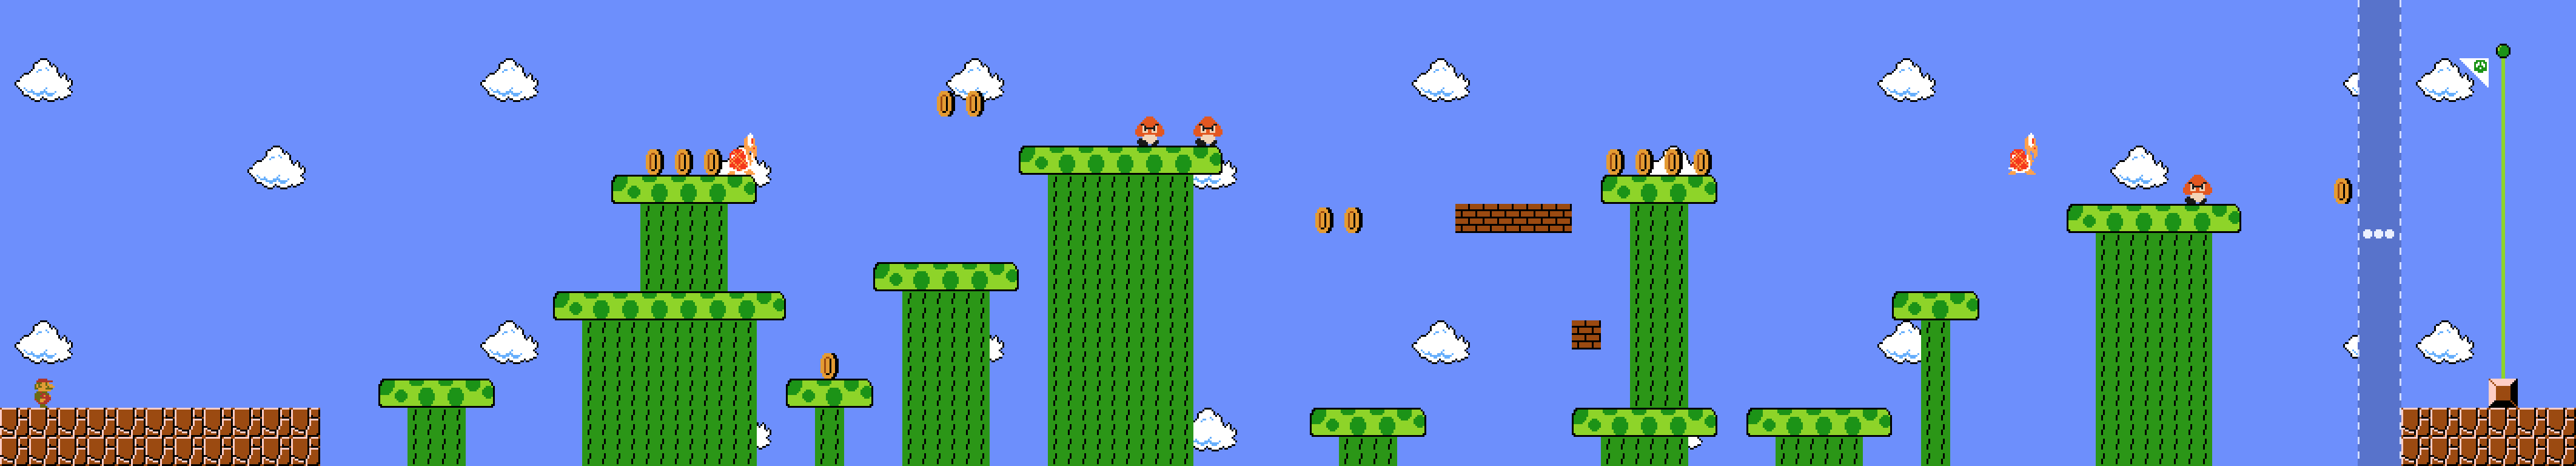
\includegraphics[width=\textwidth]{ascii-level-rendered.png}
\caption{\changed{Rendered view of the same segment.}}
\end{subfigure}

\caption{Original Super Mario Bros Level (World~1-1 segment).
         \texttt{M} marks Mario's spawn; \texttt{X} is solid ground; \texttt{U} and \texttt{S}
         are question blocks; \texttt{g} is a Goomba;
         \texttt{F} denotes level exit; \texttt{-} is empty air.}
\label{fig:ascii-level}
\end{figure}

\subsection{Level Validation}
\label{subsec:sd-level-validation}

Every submitted level undergoes format validation before insertion into the database. The
validation procedure, implemented in the backend's \texttt{seed.py} module, checks:

\begin{enumerate}
    \item \textbf{Height bounds:} the number of rows must satisfy
          $10 \leq h \leq 20$.
    \item \textbf{Width bounds:} the number of columns must satisfy
          $150 \leq w \leq 250$.  In practice, all submitted generators produce levels
          with widths between 150 and 208 columns; \KOT{??} \changed{the lower bound of 150
          corresponds to the standard screen width of the original Super Mario Bros}.
    \item \textbf{Rectangular shape:} all rows must have identical length.
    \item \textbf{Character whitelist:} every character must belong to the set of
          37 allowed tiles (Table \ref{tab:tile-legend}).
\end{enumerate}

Levels that fail any check are rejected with a descriptive error message. Note that the
platform performs \emph{format-level} validation only; there is no automated playability
or reachability analysis (e.g.\ checking that the exit is reachable from the spawn).
Content hashes are computed for deduplication.

\section{Battle and Voting System}
\label{sec:sd-battle}

The core user experience is the \emph{battle}: a blind A/B test in which the player
compares two levels produced by different generators, not knowing which generator
produced which level.

\subsection{Battle Flow}
\label{subsec:sd-battle-flow}

A battle proceeds through five stages:

\begin{enumerate}
    \item \textbf{Battle request.} The frontend calls \texttt{POST /v1/battles:next}.
    \item \textbf{Matchmaking.} The AGIS algorithm (Section \ref{sec:sd-matchmaking})
          selects two generators; one random level is drawn from each.
    \item \textbf{Gameplay.} The player plays both levels sequentially (labelled ``Left''
          and ``Right''). During play, the engine records a trajectory of Mario's position
          and death events.
    \item \textbf{Voting.} After completing both levels, the player chooses one of four
          options: \emph{Left is Better}, \emph{Right is Better}, \emph{Tie}, or
          \emph{Skip}. The ``Skip'' option, used when the player feels unable to judge or
          encounters a technical issue, does not affect ratings.
    \item \textbf{Rating update.} The backend updates Glicko-2 ratings for both generators
          atomically within a database transaction (Section \ref{sec:sd-rating}).
\end{enumerate}

Figure \ref{fig:gameplay} shows the main gameplay interface. After completing both levels,
the voting panel (Figure \ref{fig:voting}) allows the player to cast their preference and
optionally tag each level.

\begin{figure}[H]
    \centering
    
\includegraphics[width=0.95\textwidth]{main_gameplay.png}
    \caption{Main gameplay view: the player experiences a procedurally generated level
             in the browser-based Mario engine.}
    \label{fig:gameplay}
\end{figure}

\begin{figure}[H]
    \centering
    
\includegraphics[width=0.90\textwidth]{voting_panel.png}
    \caption{Voting panel shown after both levels are played, with preference buttons.
             \changed{Tag selection is accessible by hovering over the level
             (see Figure~\ref{fig:tag-selection}).}\KOT{tag selection part is not visible onthis screen actually}}
    \label{fig:voting}
\end{figure}

\begin{figure}[H]
    \centering
    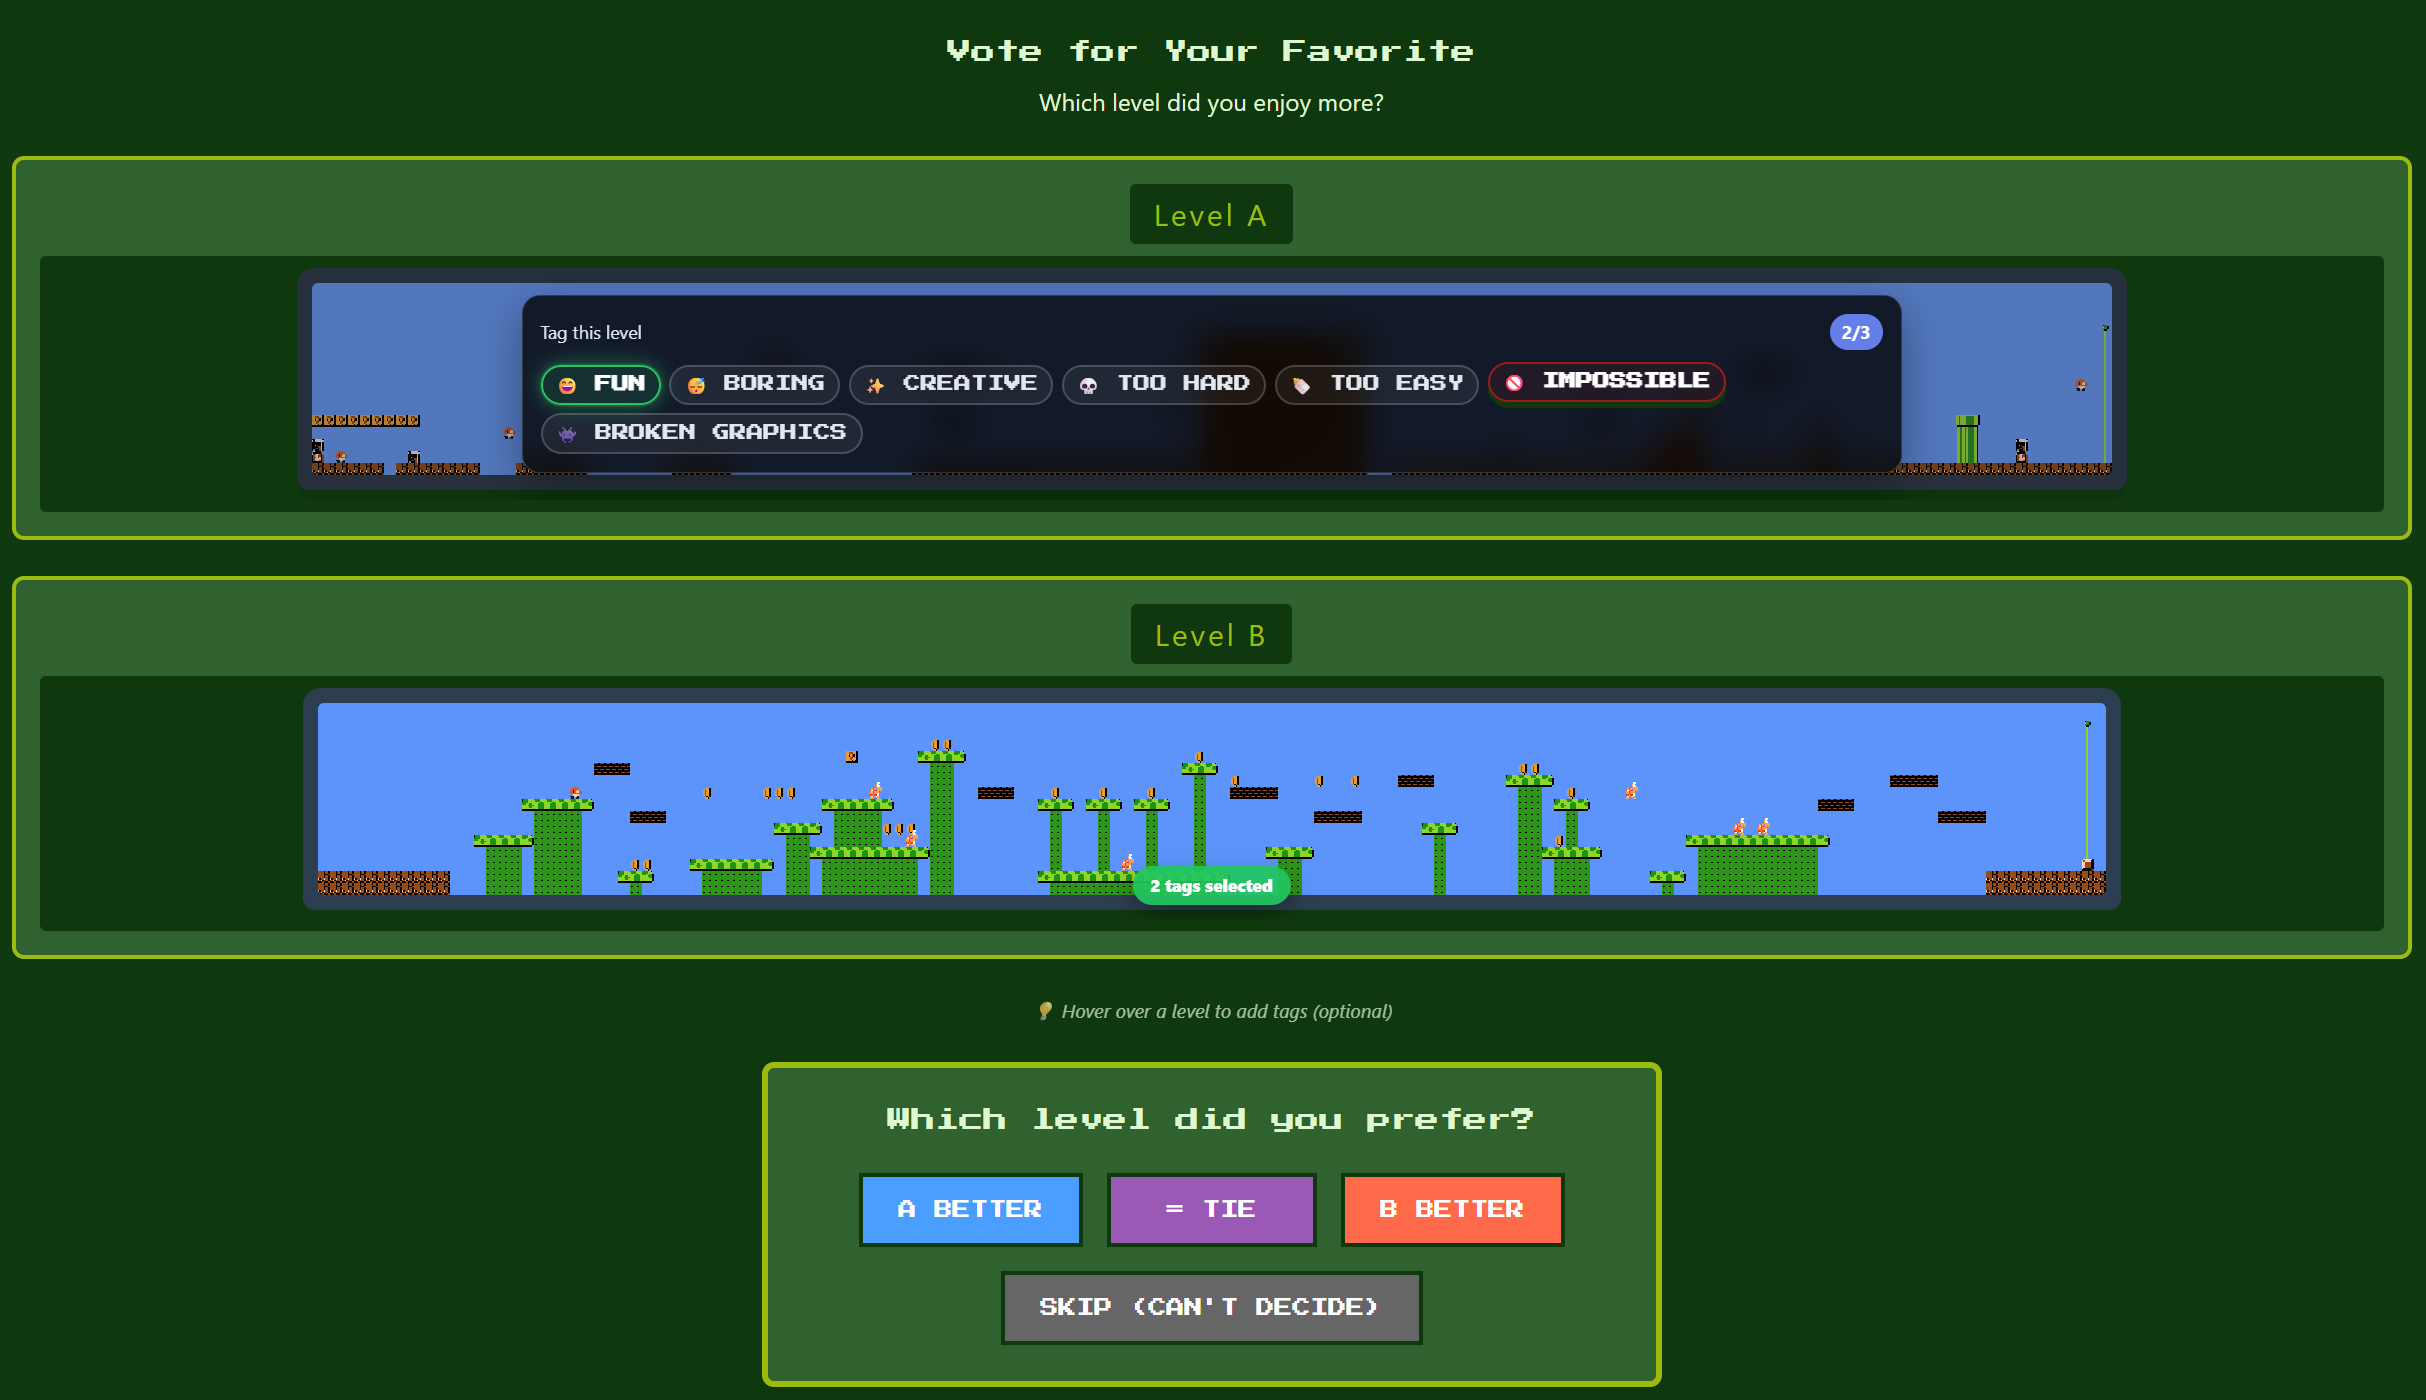
\includegraphics[width=0.90\textwidth]{tag_selection.png}
    \caption{\changed{Tag selection popup shown when the player hovers over a level.
             Players may assign up to three descriptive labels per level.}}
    \label{fig:tag-selection}
\end{figure}

\subsection{Tagging System}
\label{subsec:sd-tagging}

In addition to the preference vote, players may optionally tag each level in the battle
with up to three descriptive labels drawn from a fixed vocabulary of seven tags.
\changed{The tags were hand-crafted based on properties a PCG researcher would
want a generator to be judged on: overall enjoyment, engagement, creativity,
difficulty calibration, playability, and visual correctness. We did not find
a pre-existing tag taxonomy for PCG level evaluation in the literature; the
set was designed to be small enough for rapid annotation yet expressive enough
to capture the most salient quality dimensions.}

\begin{table}[H]
\centering
\begin{tabular}{ll}
\toprule
\textbf{Tag} & \textbf{Description} \\
\midrule
\texttt{fun}              & The level was enjoyable to play \\
\texttt{boring}           & The level lacked engagement \\
\texttt{creative}         & The level showed novel or interesting design \\
\texttt{too\_hard}        & The level was excessively difficult \\
\texttt{too\_easy}        & The level was trivially easy \\
\texttt{impossible}       & The level appeared to be uncompletable \\
\texttt{broken\_graphics} & The level had visual or rendering issues \\
\bottomrule
\end{tabular}
\caption{The seven available tags for level characterisation.}
\label{tab:tags}
\end{table}

Tags are stored as boolean columns in the \texttt{votes} table and aggregated in
\texttt{level\_stats}, enabling analyses such as correlating perceived difficulty with
win rates or identifying generators whose levels are consistently tagged as
\texttt{impossible}.

\section{Matchmaking: AGIS Algorithm}
\label{sec:sd-matchmaking}

\subsection{Problem Definition}
\label{subsec:sd-matchmaking-problem}

Given $n$ generators with current Glicko-2 ratings and uncertainties, the matchmaking
problem is to select a pair for the next battle that maximises information gain toward
accurate final rankings. Naive strategies are suboptimal:

\begin{itemize}
    \item \textbf{Uniform random} wastes battles on already-converged pairs.
    \item \textbf{Most-uncertain-first} neglects head-to-head comparisons between
          similarly rated generators.
    \item \textbf{Round-robin} ignores rating information and pairs dissimilar generators.
\end{itemize}

To address these shortcomings, we designed \textbf{AGIS (Adaptive Glicko-Informed
Selection)}, a custom two-stage matchmaking algorithm that incorporates rating
uncertainty, skill similarity, and pairwise coverage into generator selection.
While the individual components draw on well-known ideas from information-theoretic
experimental design (uncertainty sampling, coverage balancing), their combination
into a lightweight, Glicko-2-aware matchmaker tailored to the PCG evaluation setting
is, to our knowledge, novel.

\subsection{Stage 1: First Generator Selection}
\label{subsec:sd-agis-stage1}

Each generator $i$ receives a selection weight $w_i$ composing an uncertainty term and
a games-played term:

\begin{equation}
\label{eq:agis-w1}
w_i = \bigl(1 + \widetilde{\text{RD}}_i\bigr)^2 \;\cdot\; \text{boost}(\text{games}_i)
\end{equation}

where $\widetilde{\text{RD}}_i = (\text{RD}_i - \text{RD}_{\min}) / (\text{RD}_{\max} -
\text{RD}_{\min})$ is the normalised rating deviation. The \changed{\emph{boost}}\KOT{boost też zmienionym fontem} function provides a $4\times$
weight multiplier for generators with zero games, linearly decaying to $1\times$ at
\texttt{MIN\_GAMES} (default: 30). After convergence, a mild quality bias is applied:

\begin{equation}
\text{boost}_{\text{converged}} = 0.8 + q_{\text{bias}} \cdot
\min\!\Bigl(1,\;\max\!\bigl(0,\;\tfrac{\mu_i - 600}{800}\bigr)\Bigr)
\end{equation}

where $q_{\text{bias}} = 0.2$ is the configurable quality bias strength. The weights
are normalised to sum to 1, forming a categorical (discrete) probability distribution;
the first generator is then drawn from this distribution via weighted random sampling.

\subsection{Stage 2: Second Generator Selection}
\label{subsec:sd-agis-stage2}

The intuition behind Stage 2 is that the most informative battle is one between
generators of \emph{similar} strength (maximising discriminative power) whose ratings
are still \emph{uncertain} (maximising information gain per battle), while ensuring
that every pair accumulates enough head-to-head data for a reliable confusion matrix.
The four weighted components below formalise these intuitions.

Given the first generator $g_1$, the second is selected using a composite pair weight:

\begin{equation}
\label{eq:agis-w2}
w_{1,j} = \alpha \cdot S(g_1, g_j) \;+\; \beta \cdot U(g_j) \;+\;
           \gamma \cdot I(g_1, g_j) \;+\; \text{cov}(g_1, g_j)
\end{equation}

The four components are:

\begin{itemize}
    \item \textbf{Rating similarity} $S(g_1, g_j) = \exp\!\bigl(-\Delta\mu^2 / 2\sigma_s^2\bigr)$,
          a Gaussian kernel with $\sigma_s = 150$ penalising large rating gaps.
    \item \textbf{Uncertainty} $U(g_j) = 1 + \widetilde{\text{RD}}_j$, favouring
          uncertain generators (range $[1, 2]$).
    \item \textbf{Information gain} $I(g_1, g_j)$, incorporating the joint RD
          and a match-quality estimate.
    \item \textbf{Coverage bonus} $\text{cov}(g_1, g_j)$: for pairs with fewer than
          \texttt{TARGET\_BATTLES\_PER\_PAIR} (default: 10) battles, an exponential
          bonus $2 \cdot e^{-c/3}$ is applied, where $c$ is the current battle count;
          otherwise a residual $0.1$ is used.
\end{itemize}

\subsection{Parameters}
\label{subsec:sd-agis-params}

Table \ref{tab:agis-params} lists the configurable AGIS parameters and their defaults,
which are set via environment variables.

\begin{table}[H]
\centering
\begin{tabular}{llr}
\toprule
\textbf{Parameter} & \textbf{Description} & \textbf{Default} \\
\midrule
$\alpha$ & Rating similarity weight & 0.5 \\
$\beta$  & Uncertainty weight       & 0.3 \\
$\gamma$ & Information gain weight  & 0.2 \\
\texttt{MIN\_GAMES}            & Games before ``converged''  & 30 \\
\texttt{TARGET\_BATTLES\_PER\_PAIR} & Min.\ battles per pair & 10 \\
\texttt{RATING\_SIGMA}        & Similarity kernel $\sigma_s$ & 150.0 \\
\texttt{QUALITY\_BIAS}        & Quality bias strength $q_{\text{bias}}$ & 0.2 \\
\bottomrule
\end{tabular}
\caption{AGIS algorithm parameters and default values.}
\label{tab:agis-params}
\end{table}

\section{Glicko-2 Rating System}
\label{sec:sd-rating}

PCG Arena uses the Glicko-2 rating system \cite{glickman2012glicko2} to maintain
uncertainty-aware rankings. Each generator carries three parameters:

\begin{itemize}
    \item \textbf{Rating ($\mu$):} the skill estimate, displayed on a scale centred at 1000.
    \item \textbf{Rating Deviation (RD, $\phi$):} the uncertainty in the rating. High RD
          indicates an unreliable estimate; low RD indicates a well-established rating.
    \item \textbf{Volatility ($\sigma$):} the expected fluctuation in performance over time.
\end{itemize}

\KOT{te dwie subsekcje to włąściwie była kopia tego co było już wcześniej}

\changed{The mathematical foundations of the Glicko-2 system---the Bradley-Terry
model, expected score computation, and the update equations for $\phi'$ and
$\mu'$---are presented in Section~\ref{subsec:bg-glicko2}. Here we describe the
implementation-specific aspects of how PCG Arena applies these formulas.}

\subsection{Rating Update Procedure}
\label{subsec:sd-glicko-update}

After each battle, the winning generator receives a score of 1, the loser 0, and ties
yield 0.5 for both. \changed{Using the expected score and update equations from
Section~\ref{subsec:bg-glicko2}, the implementation proceeds as follows:}

\begin{enumerate}
    \item Convert ratings to the internal Glicko-2 scale (centred at 0, divided by
          $\lambda = 173.7178$).  This constant equals $400 / \ln 10 \approx 173.7178$
          and bridges the Elo convention (400 points per tenfold win-probability change)
          with the natural logistic function used internally by Glicko-2.
    \item Compute the variance $v$ from the opponent's RD.
    \item Compute $\Delta = v \cdot g(\phi_B)(s - E)$, where $s$ is the actual score.
    \item Update volatility $\sigma'$ via the iterative Illinois algorithm
          (system constant $\tau = 0.5$).
    \item \changed{Update RD and rating using Equations~\ref{eq:glicko-rd-bg}--\ref{eq:glicko-mu-bg}.}
    \item Convert back to the display scale and clamp to $[100, 3000]$.
\end{enumerate}

All rating updates are performed atomically within a single database transaction, with
an audit record written to the \texttt{rating\_events} table.

\subsection{Configuration}
\label{subsec:sd-glicko-config}

Table \ref{tab:glicko-params} lists the Glicko-2 constants used by PCG Arena.

\begin{table}[H]
\centering
\begin{tabular}{lr}
\toprule
\textbf{Parameter} & \textbf{Value} \\
\midrule
Initial rating ($\mu_0$)       & 1000 \\
Initial RD ($\phi_0$)          & 350 \\
Initial volatility ($\sigma_0$) & 0.06 \\
System constant ($\tau$)       & 0.5 \\
Scale factor ($\lambda$)       & 173.7178 \\
Minimum RD                     & 30 \\
Maximum RD                     & 350 \\
Minimum rating                 & 100 \\
Maximum rating                 & 3000 \\
\bottomrule
\end{tabular}
\caption{Glicko-2 configuration parameters.}
\label{tab:glicko-params}
\end{table}

The RD of each generator provides a natural 95\% confidence interval for its true rating:
$\text{CI}_{95\%} = [\mu - 1.96\,\text{RD},\;\mu + 1.96\,\text{RD}]$.
However, the public leaderboard displays only the point-estimate rating; confidence
intervals are not shown on the platform's frontend.
Figure \ref{fig:leaderboard} shows the leaderboard as seen by players.

\begin{figure}[H]
    \centering
    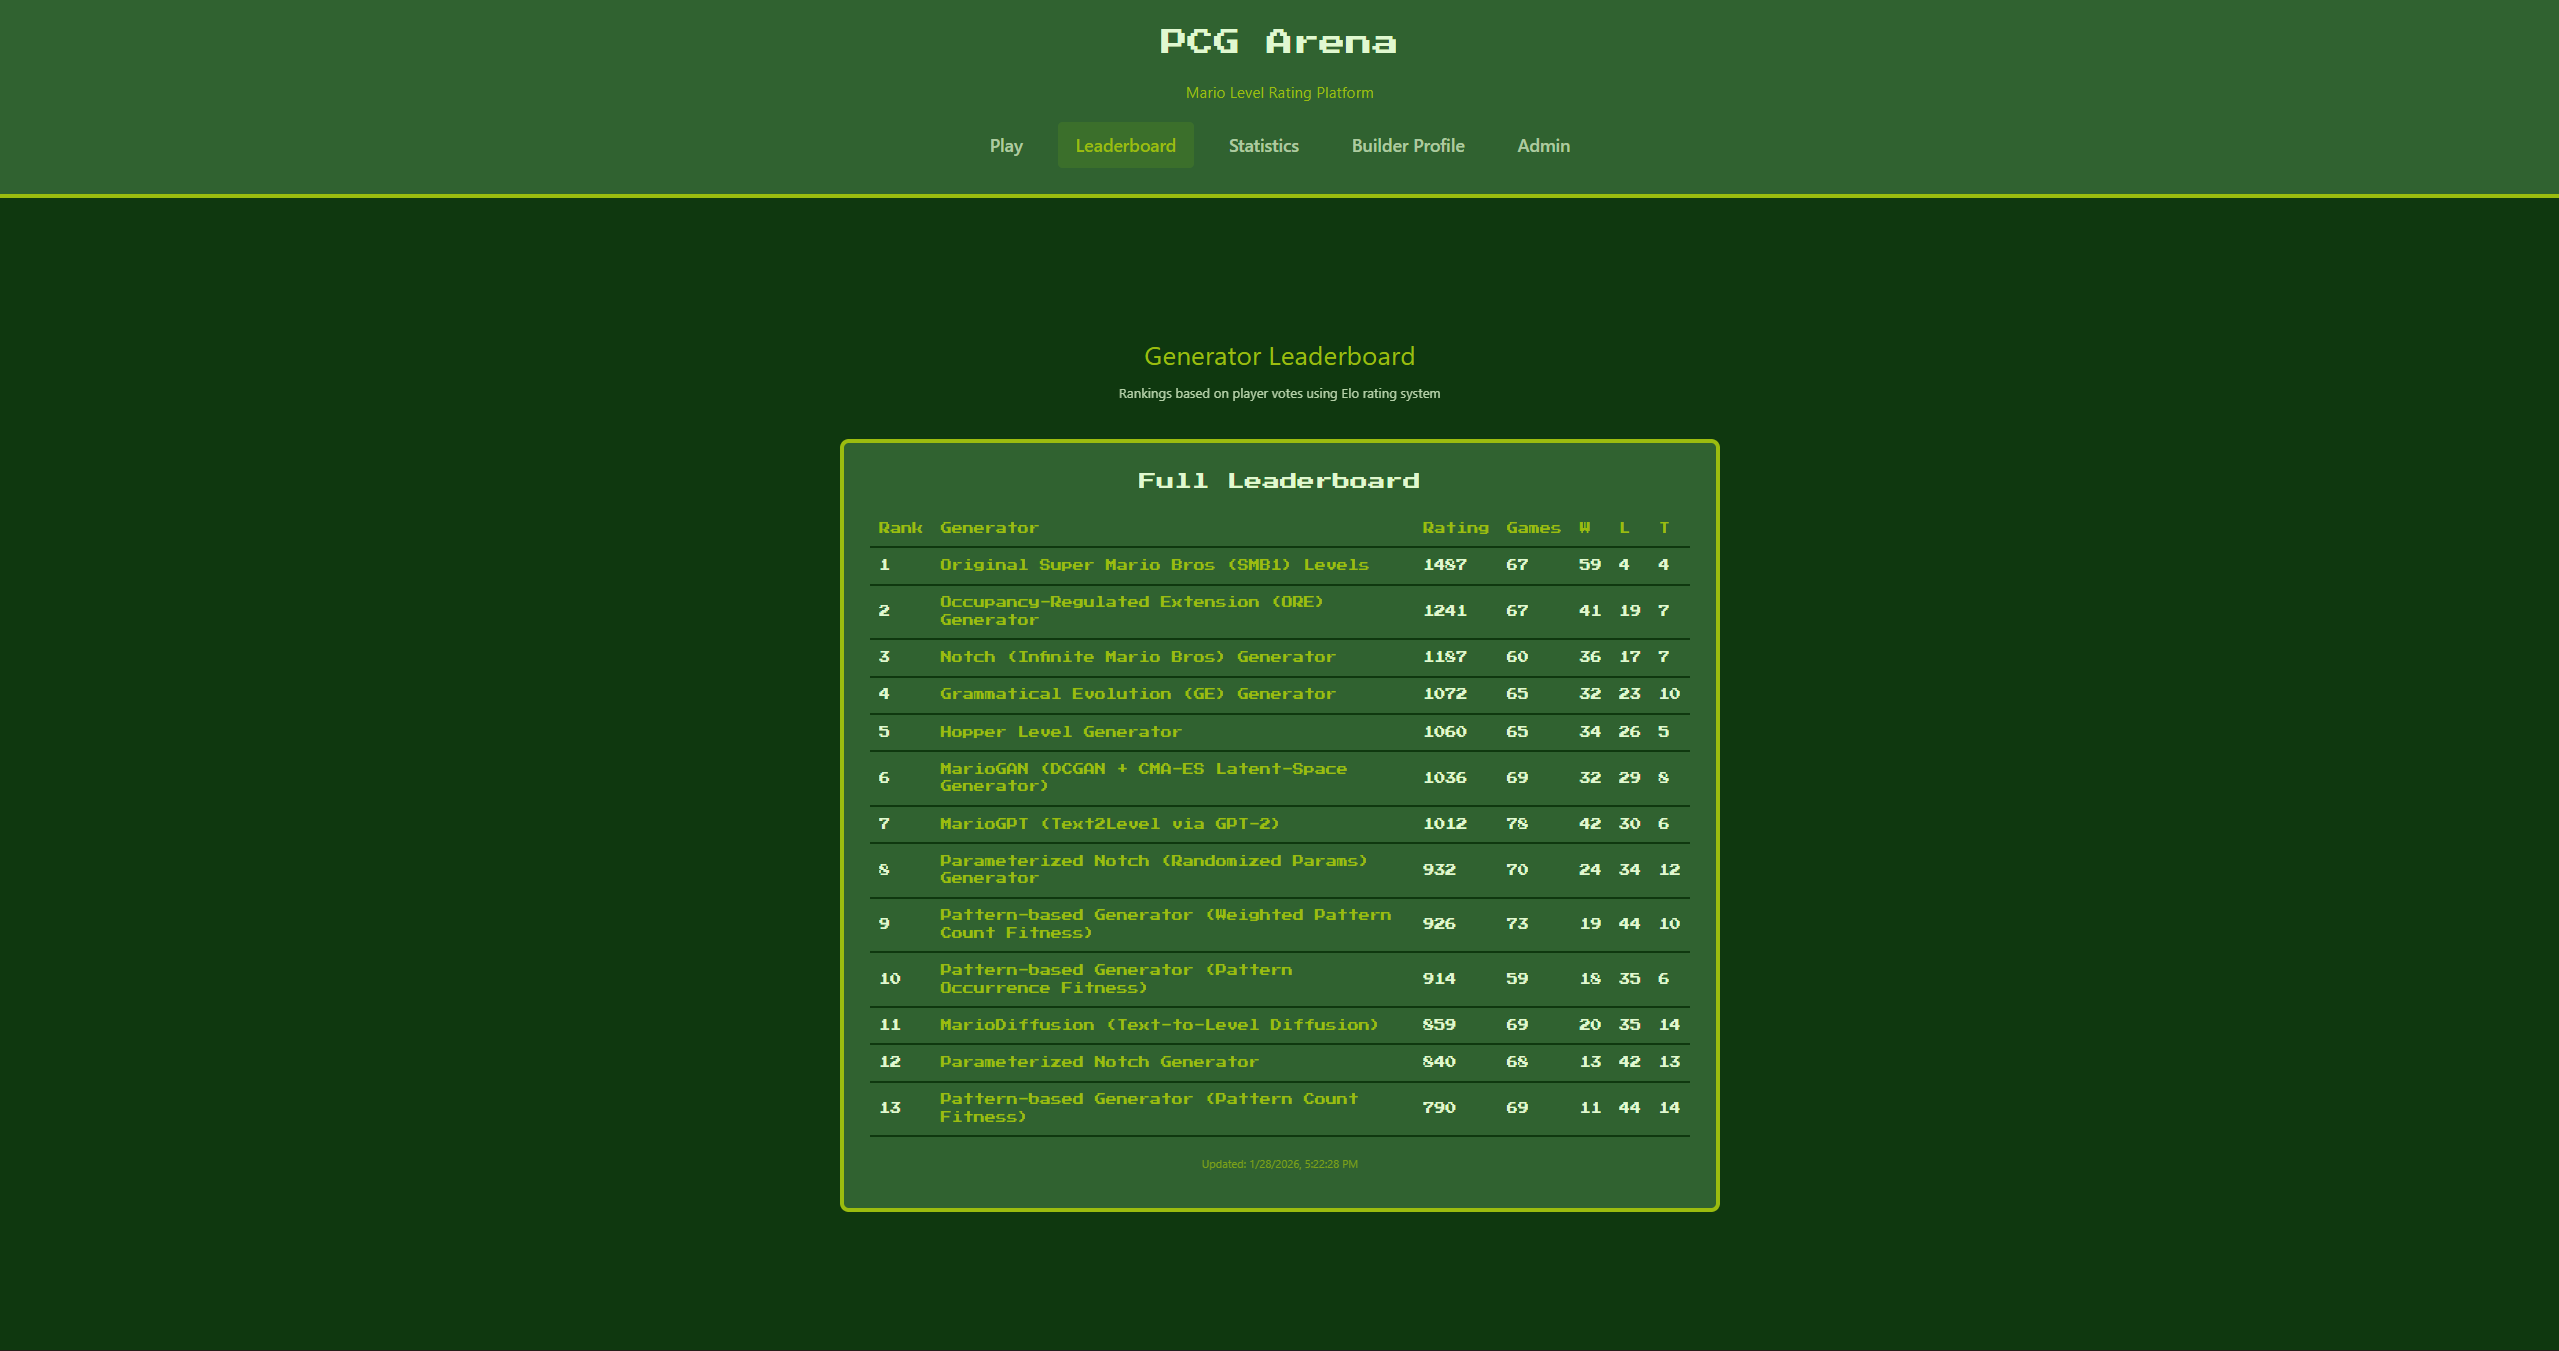
\includegraphics[width=0.95\textwidth]{leaderboard.png}
    \caption{Public leaderboard ranking generators by their Glicko-2 rating.}
    \label{fig:leaderboard}
\end{figure}

Clicking a generator reveals detailed statistics including rating history, per-opponent
win rates, a level gallery, and tag distributions
(Figure \ref{fig:generator-preview}).

\begin{figure}[H]
    \centering
    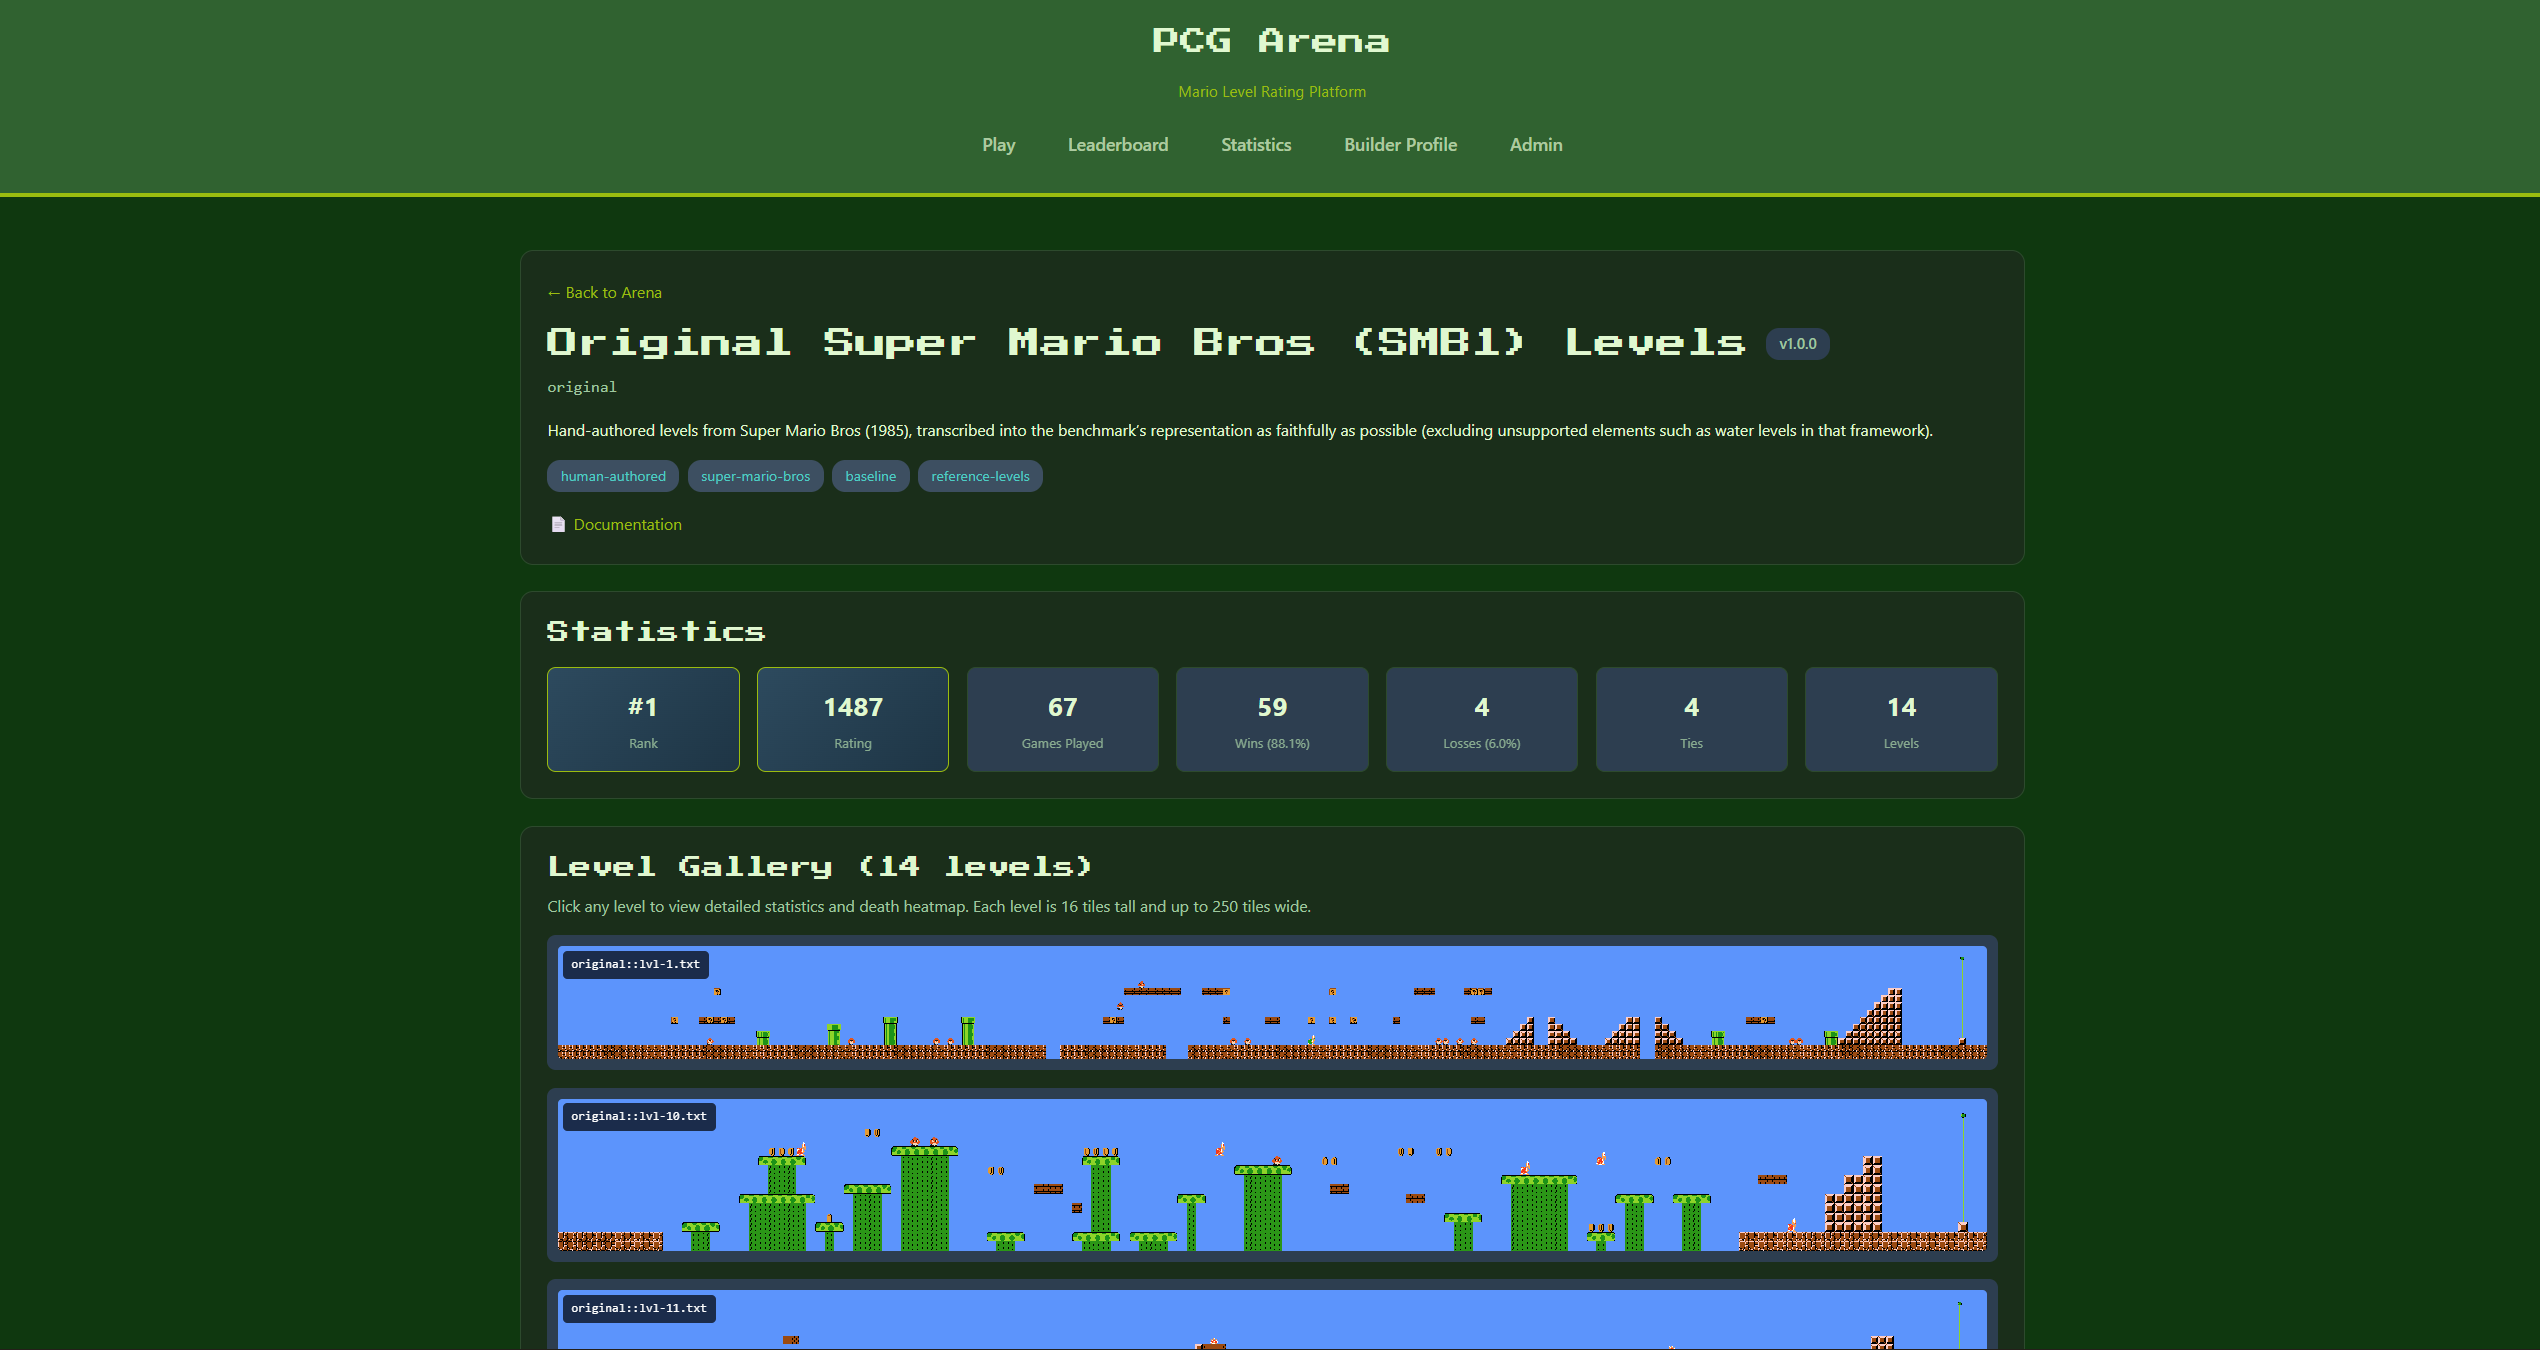
\includegraphics[width=0.95\textwidth]{generator_preview.png}
    \caption{Generator detail page showing level gallery and performance statistics.}
    \label{fig:generator-preview}
\end{figure}

\section{Builder Profile and Generator Submission}
\label{sec:sd-builder}

Authenticated users may submit their own generators through the Builder Profile page.
The submission workflow is:

\begin{enumerate}
    \item The user provides generator metadata: name, version, description, and a URL to
          the generator's source repository.
    \item The user uploads a ZIP archive containing level files in the ASCII tilemap format.
    \item The backend validates every level (Section \ref{subsec:sd-level-validation}).
          Levels that fail validation are rejected with detailed error messages.
    \item Valid levels and the generator record are inserted into the database.
    \item An initial Glicko-2 rating of $1000 \pm 350$ is assigned.
    \item The generator appears on the leaderboard immediately and enters the matchmaking
          pool.
\end{enumerate}

Each user may own at most three generators.
When a user wishes to remove a generator, the system distinguishes two cases.  If the
generator has already participated in battles, it is \emph{soft-deleted}: marked as
inactive and excluded from future matchmaking, but its records (levels, ratings, votes)
are retained so that historical analyses and the confusion matrix remain consistent.
If the generator has never appeared in a battle, it is \emph{hard-deleted} (fully
removed from the database) since no other data depends on it.

Figure \ref{fig:builder} shows the Builder Profile page.
\KOT{chyba tym wszystkim screenom by się przysłużył clip do środkowej meaningful części. Tzn ja lubię zielony, połacie zielonego po bokach mi nie przeszkadzają, ale jednak readability się pogarsza o nie pozwala trochę powiększyć obrazka żeby coś było widać na powiększeniu mniejszym niż 180}

\begin{figure}[H]
    \centering
    
\includegraphics[width=0.95\textwidth]{builder_profile.png}
    \caption{Builder Profile page for submitting and managing generators.}
    \label{fig:builder}
\end{figure}

\section{Authentication}
\label{sec:sd-auth}

PCG Arena supports two authentication methods:

\begin{itemize}
    \item \textbf{Google OAuth 2.0.} The frontend opens a Google sign-in popup; the
          returned ID token (JWT) is sent to \texttt{POST /v1/auth/google}, where the
          backend verifies it against Google's servers. Google users are automatically
          marked as email-verified.
    \item \textbf{Email and password.} Users register with an email, password, and display
          name. Passwords are hashed with bcrypt (work factor 12). A verification email
          is sent via Twilio SendGrid containing a unique token (64 hex characters,
          24-hour expiry).
\end{itemize}

Upon successful authentication, the backend issues a session cookie
(\texttt{arena\_session}) containing a 256-bit cryptographically random token. Sessions
expire after seven days. HTTP-only cookies prevent client-side script access.

Administrative access is granted to users whose email addresses appear in the
\texttt{ARENA\_ADMIN\_EMAILS} configuration list.

\section{Deployment and Infrastructure}
\label{sec:sd-deployment}

PCG Arena is deployed on Google Cloud Platform using a single Compute Engine instance
(\texttt{e2-micro}, Ubuntu 22.04 LTS). The backend runs inside a Docker container
orchestrated by \texttt{docker-compose}, with the SQLite database file bind-mounted
from the host for persistence across container rebuilds.

\noindent
Caddy serves as the reverse proxy, handling:\KOT{noindent}

\begin{itemize}[nosep]
    \item Automatic TLS certificate provisioning and renewal (Let's Encrypt).
    \item HTTP-to-HTTPS redirection.
    \item Reverse proxying API requests to \texttt{localhost:8080}.
    \item Static file serving for the frontend production build.
\end{itemize}

The platform is accessible at \texttt{https://pcg-arena.com}. The backend binds to
\texttt{127.0.0.1:8080} and is not exposed to the public internet directly; all external
traffic passes through Caddy. Firewall rules allow only ports 80 and 443. Database backups
are performed via a scheduled script that copies the SQLite file to a timestamped archive.




\chapter{User Study and Exploratory Data Analysis}
\label{ch:eda}

This chapter presents the PCG Arena data as an exploratory user study and generator characterisation, organised around five research questions:

\begin{enumerate}[nosep]
    \item \textbf{RQ1}: Which generators are preferred by players in blind pairwise comparisons?
    \item \textbf{RQ2}: How do generators differ in static expressive range, and which structural properties align with player preference?
    \item \textbf{RQ3}: What patterns of player movement appear in the recorded trajectories for each generator?
    \item \textbf{RQ4}: Are player preferences and play styles homogeneous, or do visible subgroups emerge?
    \item \textbf{RQ5}: What do tags reveal about why levels win or lose?
\end{enumerate}

The analysis is exploratory: its conclusions rely on patterns observed in the data and its visualisations rather than on formal hypothesis testing. The aim is to demonstrate what PCG Arena can measure---preference, structure, gameplay behaviour, user heterogeneity, and qualitative failure modes---while acknowledging that the current dataset is still too small to support claims of universal design laws.

% ===================================================================
\section{Study Protocol and Dataset}
\label{sec:eda-study-design}

Participants were recruited through university social-media channels, word of mouth among game-development and computer-science communities, and a small promoted Reddit campaign targeting game-development and procedural-generation communities. Participation was anonymous. The platform assigned browser-based anonymous player identifiers and session identifiers, persisted through cookies or local browser storage. Consequently, ``players'' in this analysis should be interpreted as anonymous browser/player IDs rather than verified unique humans; clearing cookies or changing device/browser could create a new ID.

Each battle used a blind A/B protocol. A player saw two levels from different generators, played one attempt on each side, and then selected the preferred side, a tie, or skip. Optional tags could be attached to either side. Restricting each side to a single attempt was a deliberate system-design decision. A protocol allowing multiple attempts per level was also implemented and tested, but limiting play to one attempt per side collects substantially more pairwise comparisons per unit of player time, directly serving the platform's main goal of building a leaderboard from a large number of A/B comparisons. For interpretation, this means the death variable is a binary failure indicator for a single side-level attempt rather than a repeated-death count.

The May 2026 analysis export contains the data summarized in Table~\ref{tab:eda-dataset}. Skip votes are included in engagement summaries but excluded from preference rankings. Ties are treated as 0.5 points for each side.

\begin{table}[H]
\centering
\caption{Dataset summary for the exploratory analysis. Player counts refer to anonymous browser/player IDs, not verified unique humans.}
\label{tab:eda-dataset}
\begin{tabular}{lr}
\toprule
\textbf{Quantity} & \textbf{Count} \\
\midrule
Vote rows analyzed & 1,000 \\
Anonymous player profiles & 79 \\
Anonymous player IDs in vote table & 77 \\
Session IDs in vote table & 213 \\
Level-stat records exported & 1,104 \\
Generator IDs in research plots & 14 \\
Per-side telemetry records & 2,000 \\
Played side records & 1,968 \\
Embedded trajectory records & 1,968 \\
Tag assignments & 329 \\
\bottomrule
\end{tabular}
\end{table}

The vote outcomes are balanced between the two screen sides (418 left wins and 398 right wins), with 165 ties and 19 skips, indicating no systematic side bias; moreover, the assignment of levels to the left or right side was randomised, further reducing the risk of positional bias. The median play duration is 8.0 seconds, but a small number of inactive-tab outliers are present; duration-dependent plots therefore use clipping or robust summaries.

% ===================================================================
\section{RQ1: Generator Preference Ranking}
\label{sec:eda-rankings}

The core purpose of PCG Arena is to measure human preference between generators. For each non-skip battle, the selected side receives score 1, the rejected side receives score 0, and ties give 0.5 to both sides. Figure~\ref{fig:eda-generator-ranking} shows the resulting generator leaderboard with bootstrap uncertainty intervals over votes.

\begin{figure}[H]
\centering

\includegraphics[width=0.95\textwidth]{eda_generator_ranking.png}
\caption{Generator ranking from blind pairwise votes. Bars show mean preference score, where win = 1, tie = 0.5, and loss = 0; horizontal intervals show bootstrap uncertainty. Bar colour encodes the generator family (human-authored, preference-trained, neural, constructive/search, and pattern-based), as shown in the in-plot legend.}
\label{fig:eda-generator-ranking}
\end{figure}

The strongest result is that the human-authored \texttt{original} baseline and \texttt{mariodpo} are nearly tied at the top. \texttt{original} scores 0.833, while \texttt{mariodpo} scores 0.832. Both are well above the neutral 0.5 line. The next tier consists of \texttt{ore} (0.655) and \texttt{mariogpt} (0.643), followed by mid-table constructive and neural generators. The pattern-based generators occupy the bottom of the ranking: \texttt{patternWeightCount} scores 0.385, \texttt{patternOccur} scores 0.284, and \texttt{patternCount} scores 0.262.

This ordering is meaningful for two reasons. First, the human-authored baseline remains a strong benchmark, which is expected if the vote data captures level quality. Second, \texttt{mariodpo} approaches the human baseline and clearly outperforms the other procedural generators in this export, suggesting that preference-aligned generation is a promising direction for the platform.

Figure~\ref{fig:eda-pairwise-confusion} gives the corresponding head-to-head matrix. Rows and columns are ordered by the ranking above. The matrix reveals that the top generators are not benefiting only from weak opponents: \texttt{original} and \texttt{mariodpo} perform well across many pairings, whereas pattern generators lose consistently across opponents.

\begin{figure}[H]
\centering
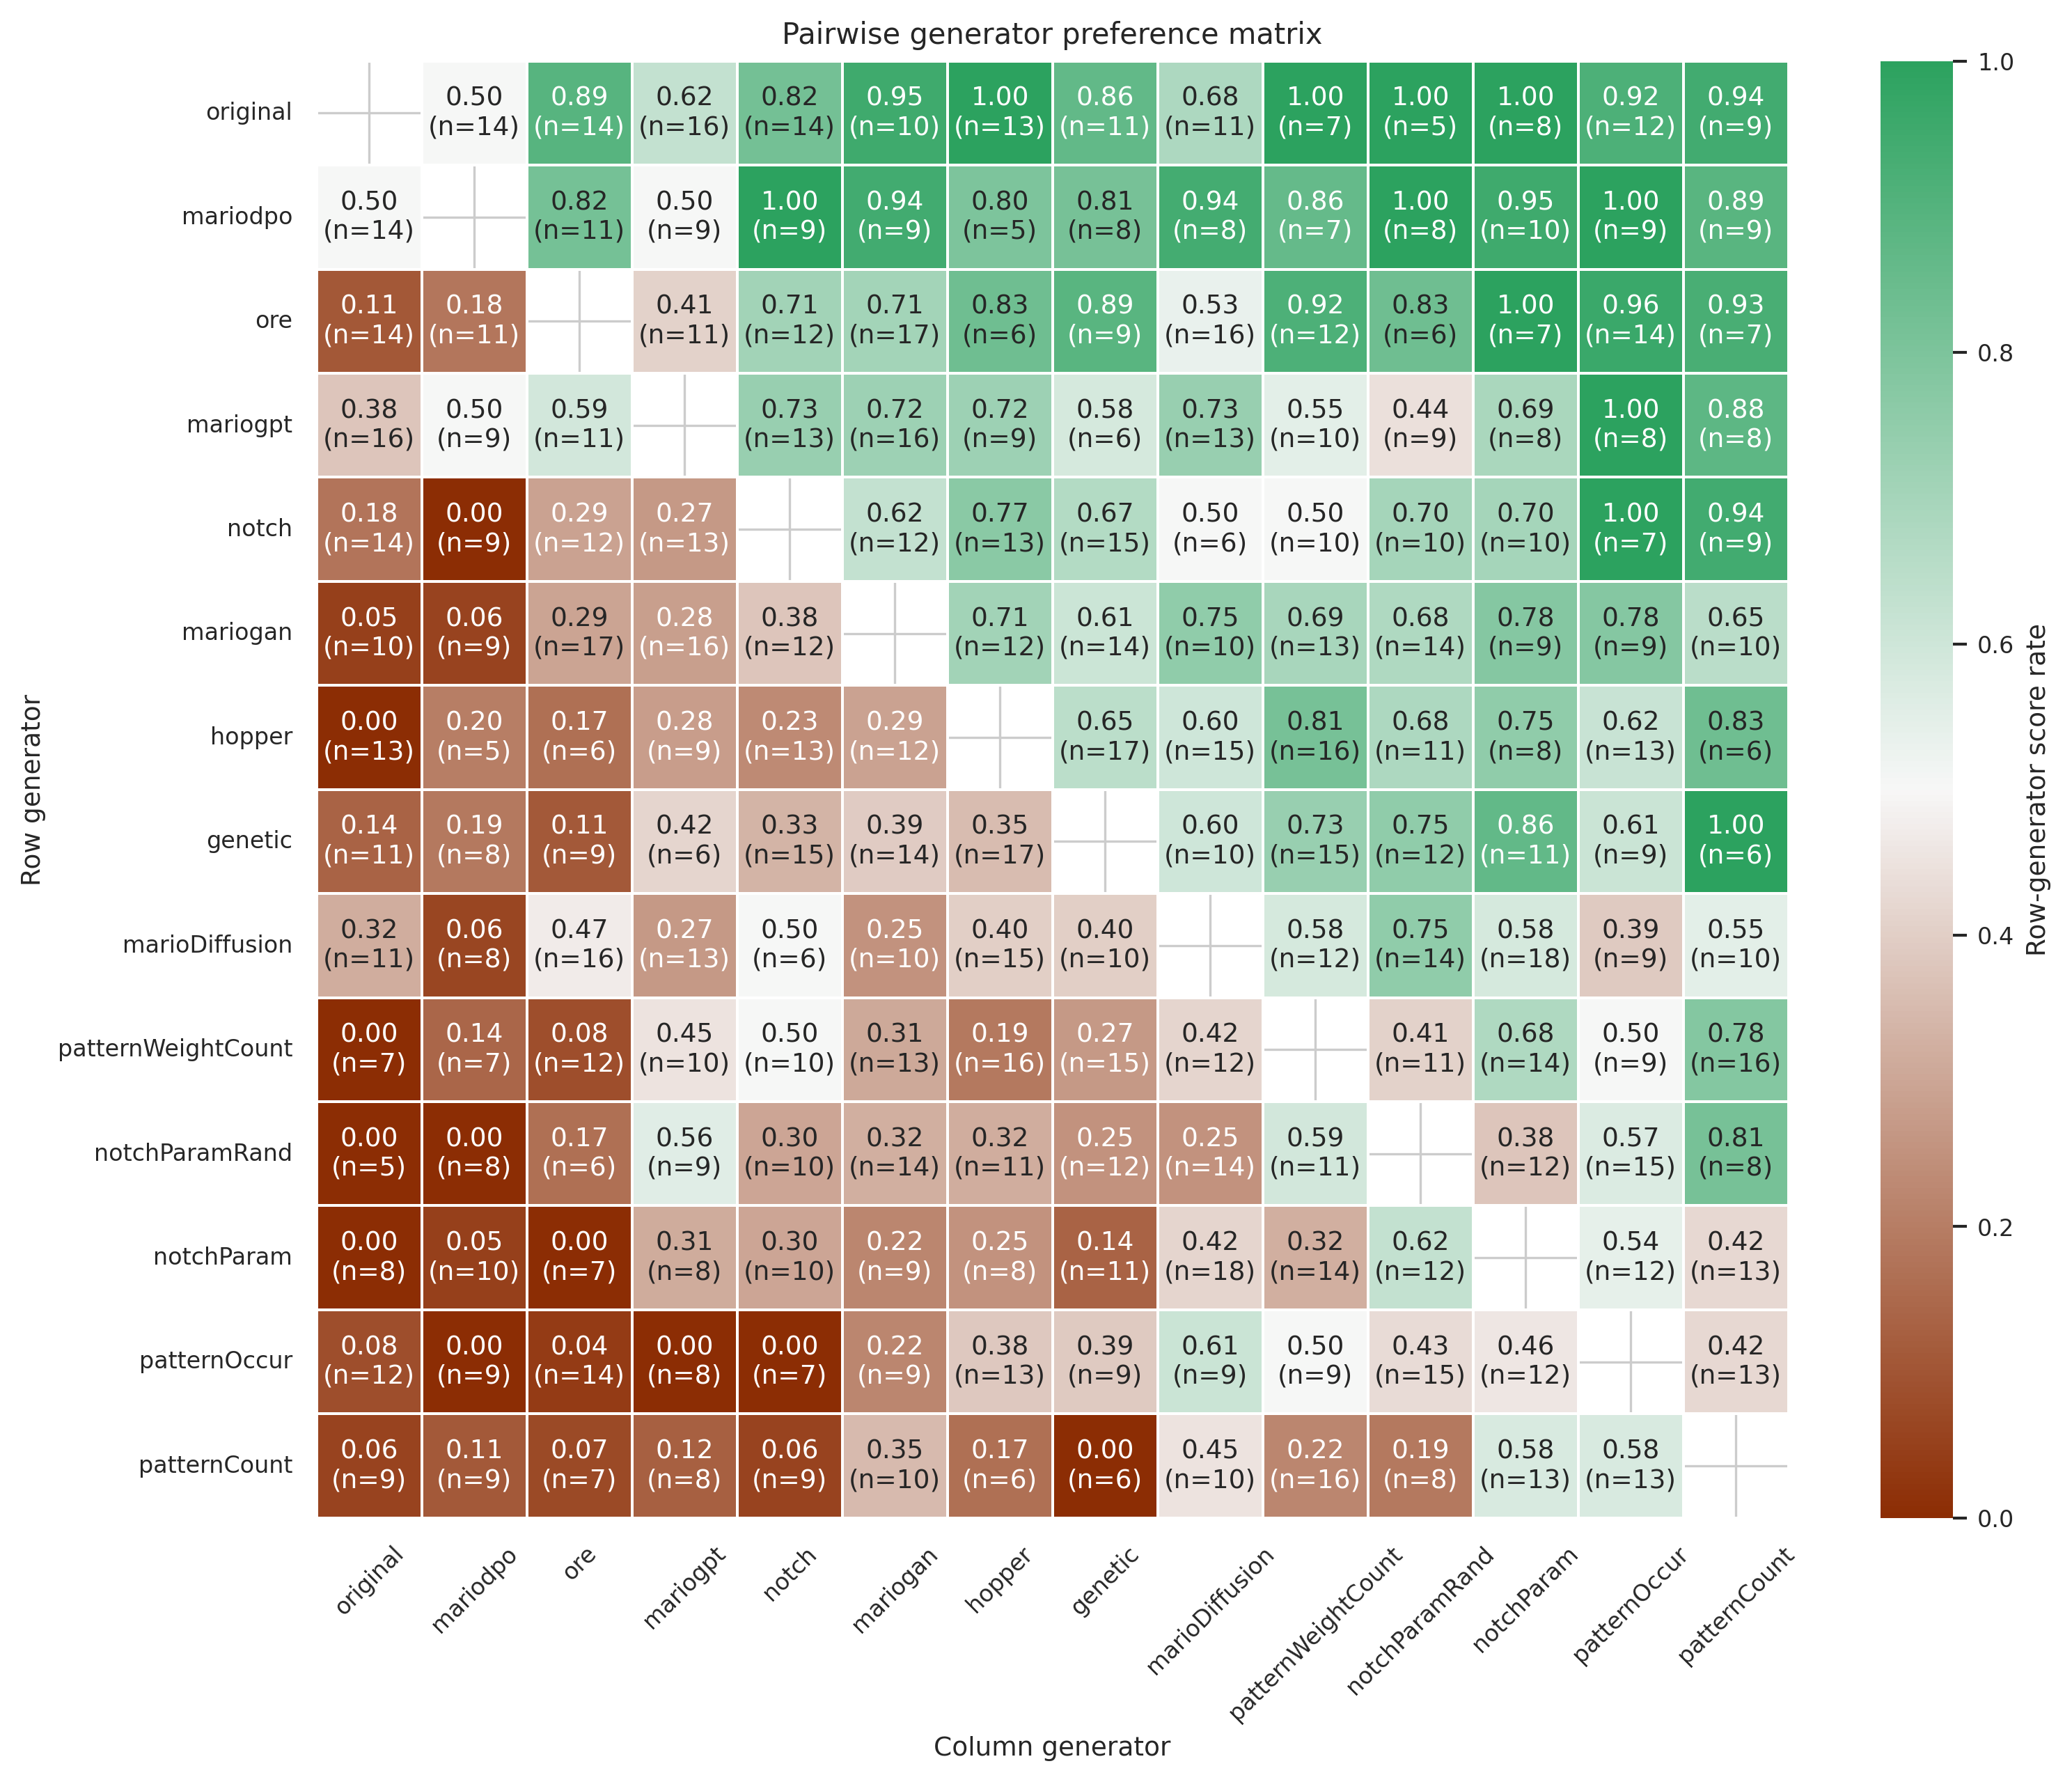
\includegraphics[width=0.95\textwidth]{eda_pairwise_confusion.png}
\caption{Pairwise generator preference matrix ordered by overall ranking. Each cell is the score rate for the row generator against the column generator, with ties counted as 0.5. Green indicates a higher score rate for the row generator.}
\label{fig:eda-pairwise-confusion}
\end{figure}

% ===================================================================
\section{RQ2: Static Expressive Range}
\label{sec:eda-static-expressive-range}

The second research question asks what we can learn about a generator by
looking at the levels themselves, without involving any player. The input is a
level as plain text (an ASCII tilemap), and the output is a small set of
numbers describing what the level looks like: how flat or hilly it is, how
many enemies it contains, how often it has gaps, how many rewards it offers,
and how similar its columns are to one another. Computing these numbers across
all generators makes it possible to compare them on a common footing and to
check whether any of these structural properties line up with the player
preference scores from RQ1.

We compute the metrics directly from the ASCII level files. Linearity is the
coefficient of determination ($R^2$) of a least-squares line fitted to the
playable surface profile; it measures how well a straight line explains the
surface, so a higher $R^2$ corresponds to flatter, more linear and more
predictable terrain, while a lower value indicates a bumpier, more irregular
profile. Density metrics count solid,
enemy, reward, and gap structure per tile or per level column. Leniency
combines gap density, enemy density, maximum gap width, rewards, and blocks
into a single descriptive score; because the various leniency definitions in
the PCG literature are not mutually comparable, we use our formulation only to
compare generators within this study, not as an absolute, cross-paper measure
of difficulty. Diversity is estimated with tile/column entropy, the unique-column
ratio, the compression ratio, and gzip normalized compression distance (NCD).

Figure~\ref{fig:eda-static-metrics-table} summarizes the main static metrics by generator. Figure~\ref{fig:eda-expressive-range} then shows each generator's expressive range in the plane of linearity and operational leniency.

\begin{figure}[H]
\centering
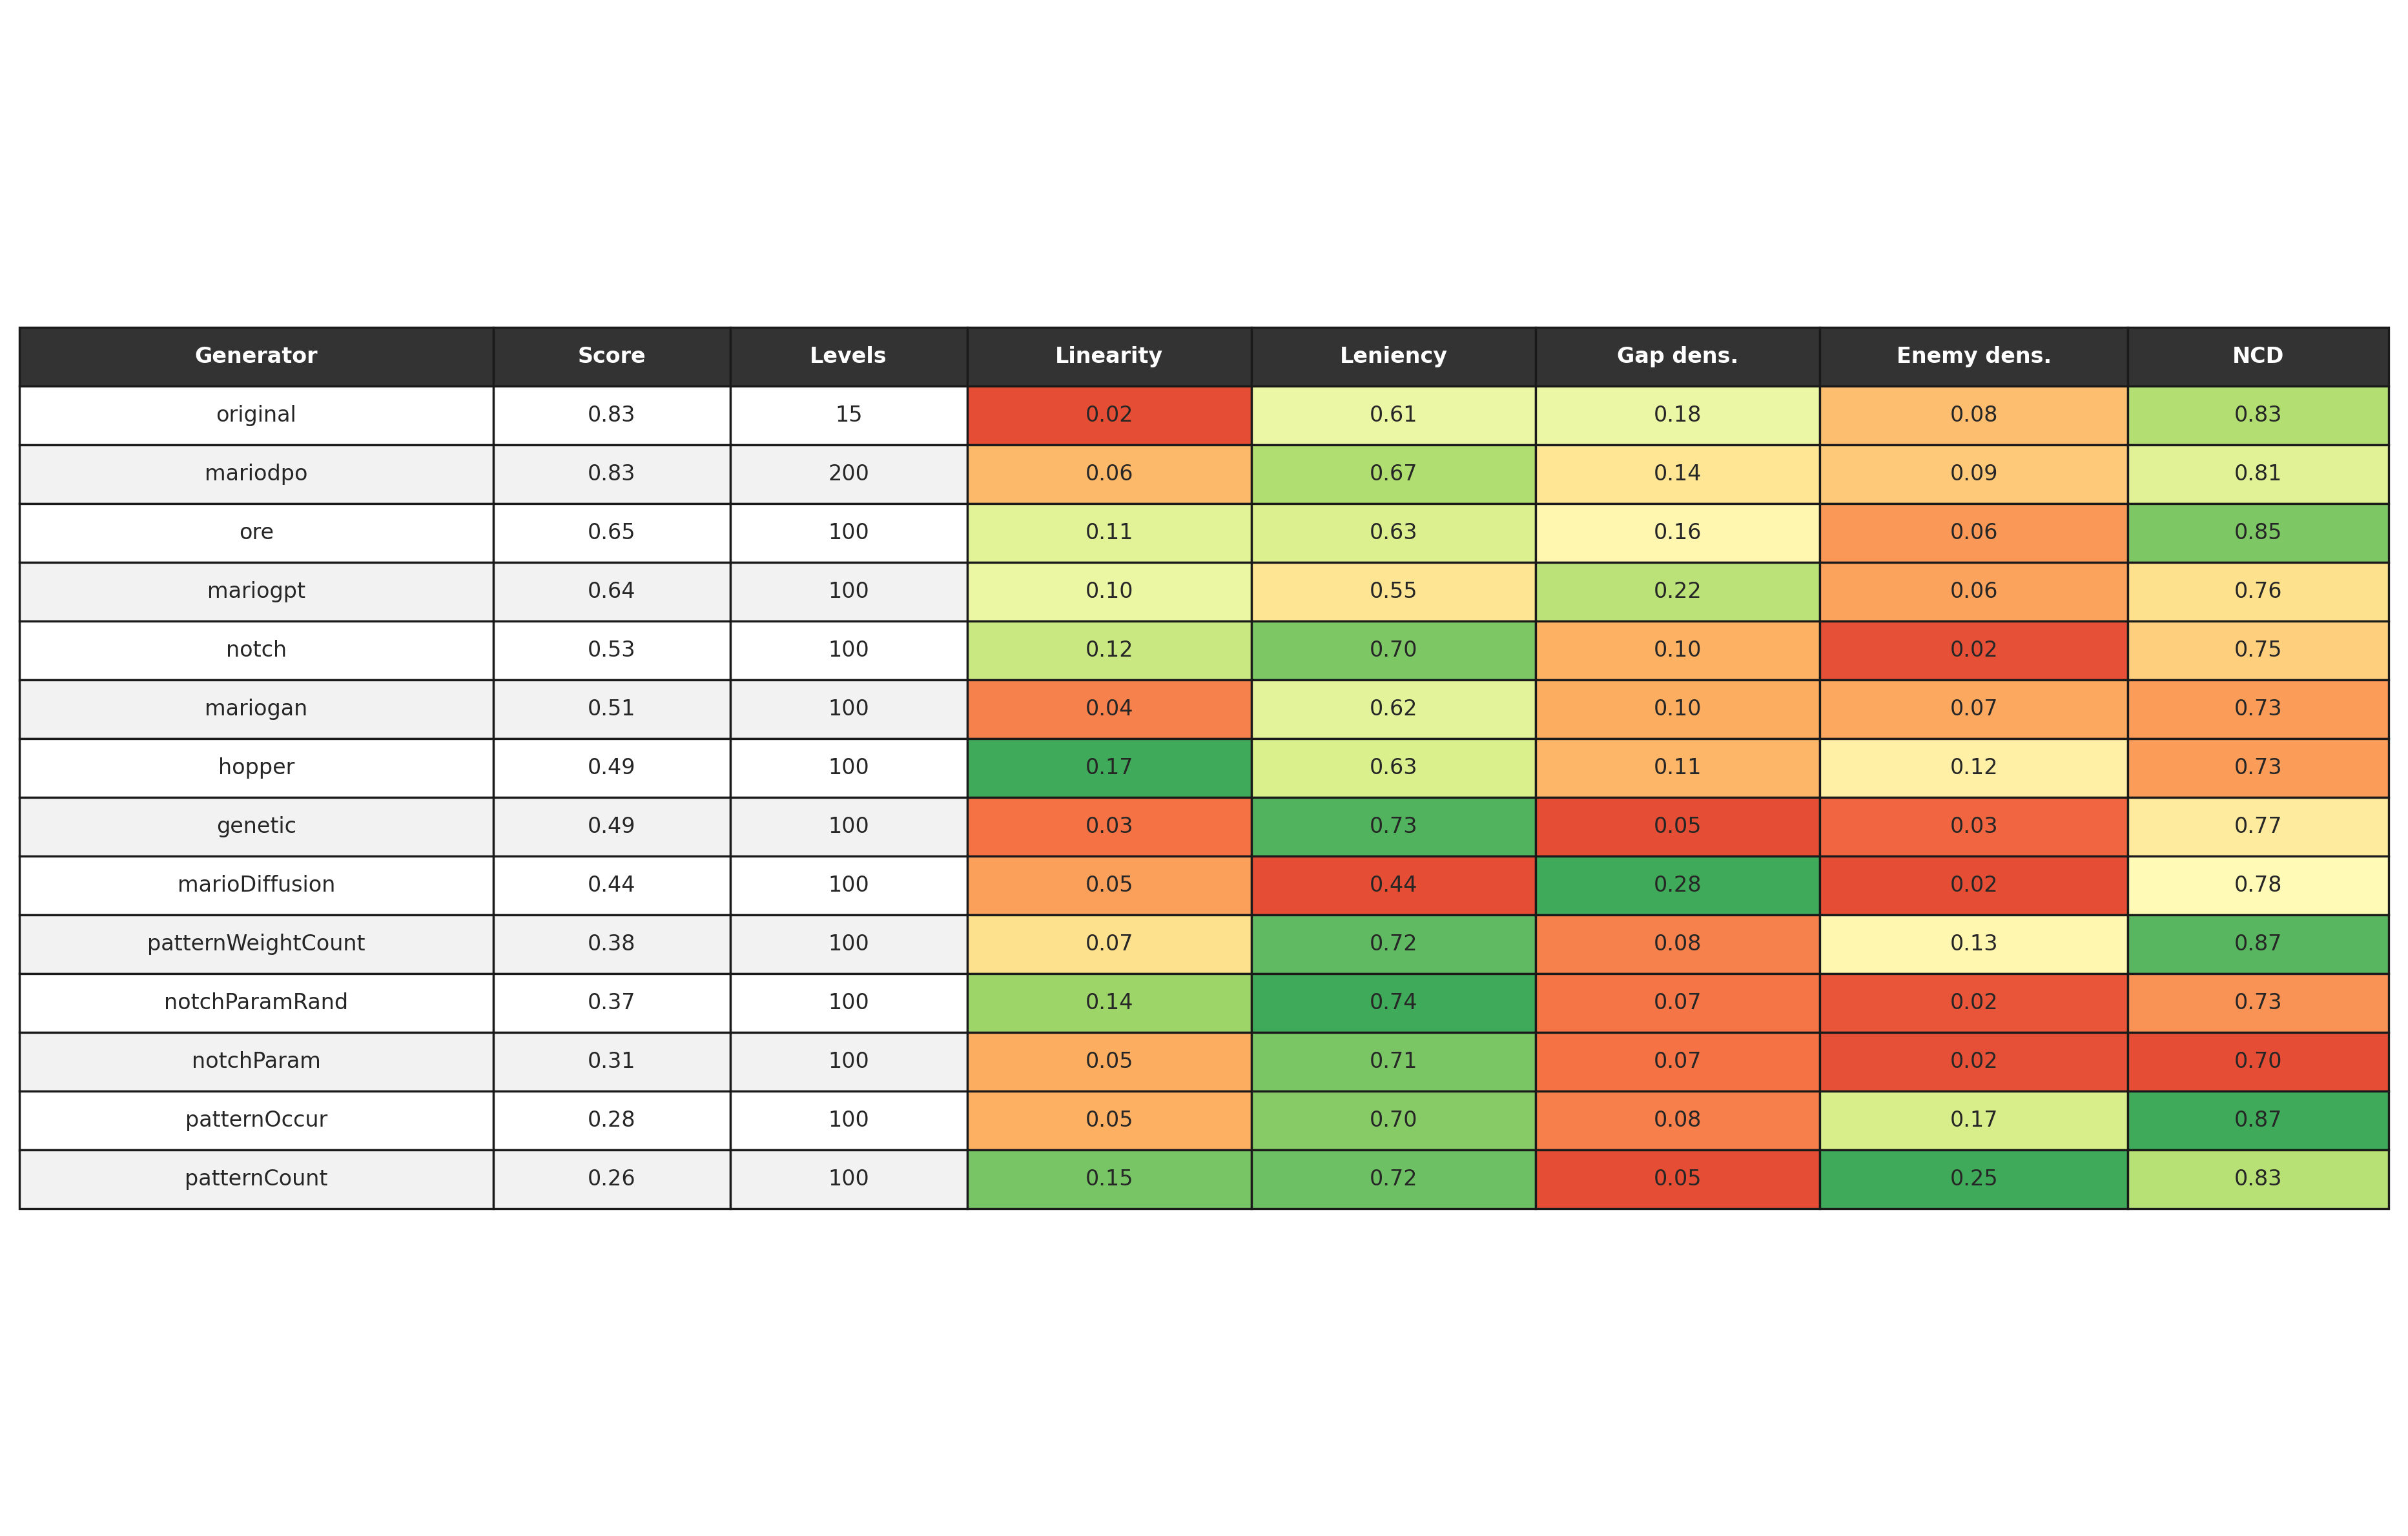
\includegraphics[width=0.95\textwidth]{eda_static_metrics_table.png}
\caption{Static expressive metrics computed from level text files. Metrics include fitted-surface linearity, operational leniency, gap density, enemy density, and within-generator compression distance. Each of the five metric columns is shaded within the column from red (low) to green (high) as a visual reading aid.}
\label{fig:eda-static-metrics-table}
\end{figure}

\begin{figure}[H]
\centering
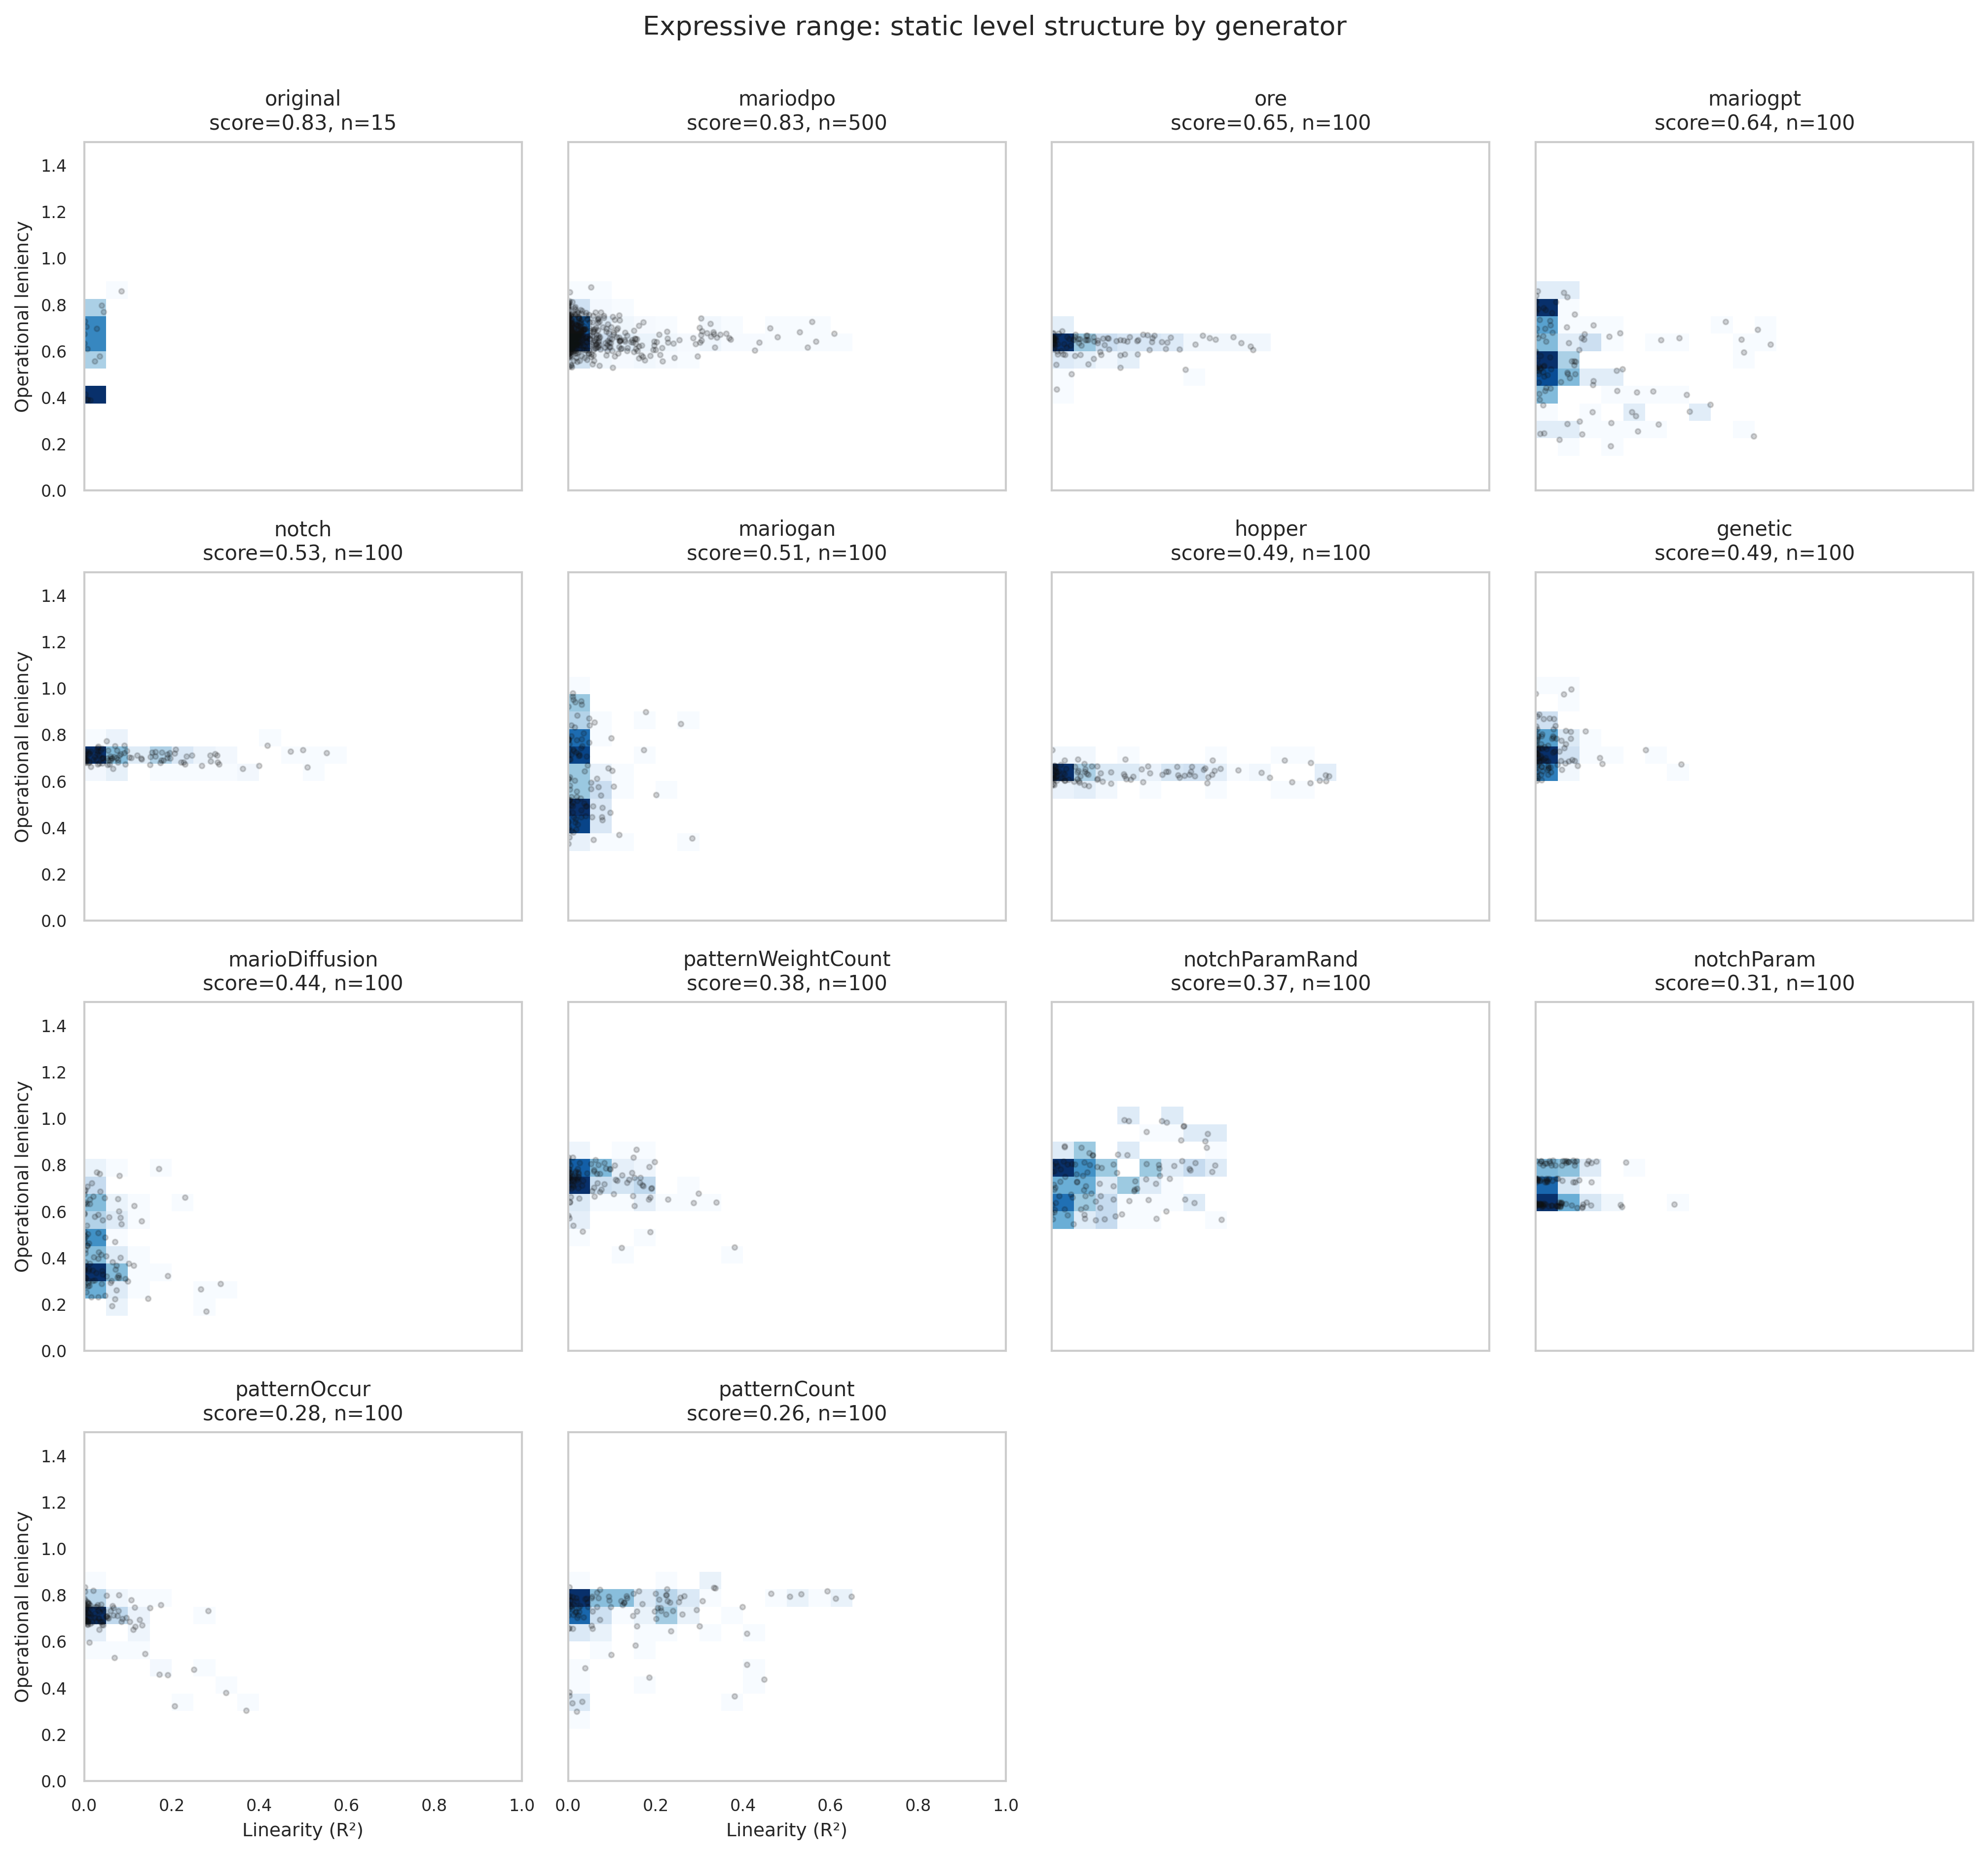
\includegraphics[width=\textwidth]{eda_expressive_range.png}
\caption{Expressive-range view of static level structure. Each subplot shows levels from one generator in the linearity--leniency plane, ordered by preference ranking.}
\label{fig:eda-expressive-range}
\end{figure}

Taken together, the two figures show several consistent patterns. The
high-ranked generators \texttt{original}, \texttt{mariodpo}, \texttt{ore} and
\texttt{mariogpt} are the only ones that combine non-trivial reward density
with a moderate amount of gaps and enemies: there is something to collect, and
there is some, but not too much, danger. The pattern-based generators sit at
the opposite extreme. They produce zero rewards and the highest enemy density
in the corpus, and on the expressive-range scatter their levels collapse into
a narrow strip dominated by gaps and obstacles. Even when their leniency score
looks moderate, this is a side-effect of having very few power-ups and little
structural variety rather than evidence of a well-balanced design. Constructive
generators such as \texttt{notch}, \texttt{notchParam} and \texttt{notchParamRand}
lie in between: they offer flat, easy ground with low enemy density, but
essentially no rewards, which is consistent with them being safe but bland.
Finally, \texttt{ore} stands out as the most structurally diverse generator,
with the highest unique-column ratio and the highest within-generator NCD,
which helps explain why it climbs into the top tier despite using a much
simpler chunk-based assembly approach than the neural generators.

Figure~\ref{fig:eda-static-vs-rating} relates selected structural summaries to preference score. With only 14 generators, these plots should be read as showing the direction and rough strength of each association, not as formal statistical tests. Reward density and unique-column ratio show the clearest positive association with preference score in this export, while distance from the \texttt{original} corpus by NCD is negatively associated with preference. Crucially, however, no single metric explains the ranking on its own: the better predictors still have visible exceptions, and difficulty proxies such as enemy density show no consistent relationship with preference at all. This is precisely the difficulty that motivates PCG Arena---player preference is a multi-dimensional signal that no individual static metric captures, which is why direct human comparison, rather than any automated proxy, is needed to rank generators reliably.

\begin{figure}[H]
\centering
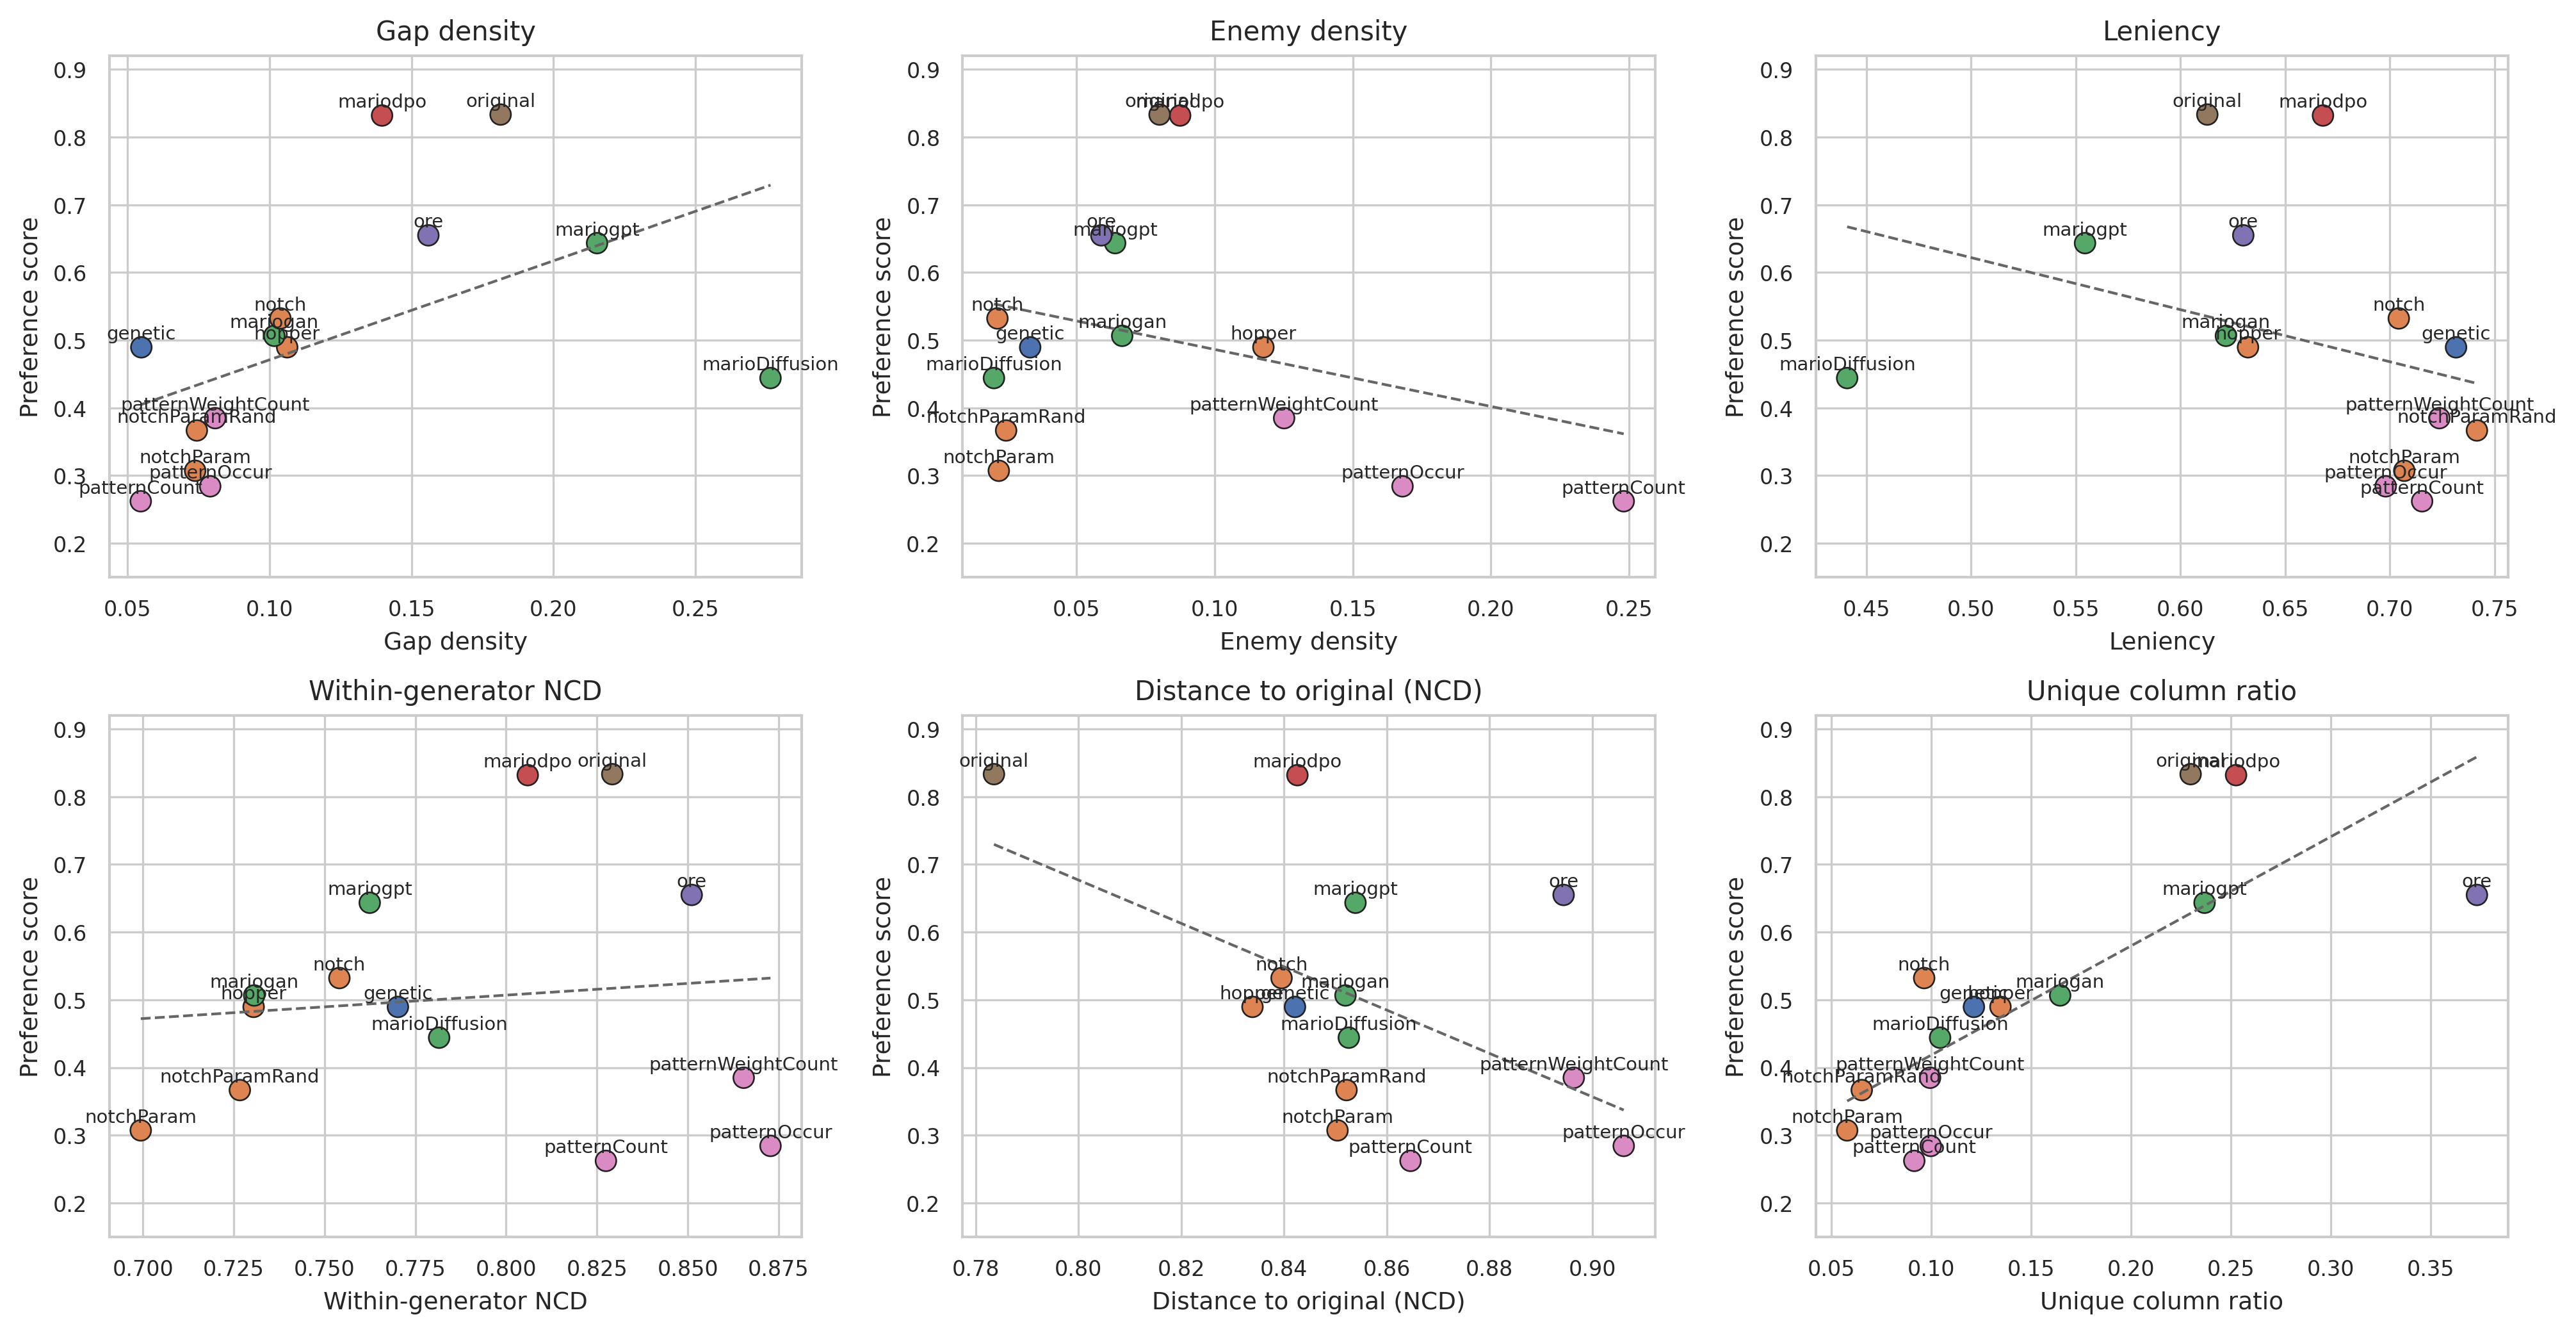
\includegraphics[width=\textwidth]{eda_static_metrics_vs_rating.png}
\caption{Generator preference score against selected static metrics. The fitted lines are descriptive trend guides, not causal claims.}
\label{fig:eda-static-vs-rating}
\end{figure}

% ===================================================================
\section{RQ3: Gameplay Trajectory Fingerprints}
\label{sec:eda-trajectory-fingerprints}

For each generator, Figure~\ref{fig:eda-trajectory-stacks} overlays all recorded Mario paths as thin red traces. This plot is intentionally simple: it shows where players actually moved in levels from each generator under the one-attempt battle protocol.

\begin{figure}[H]
\centering
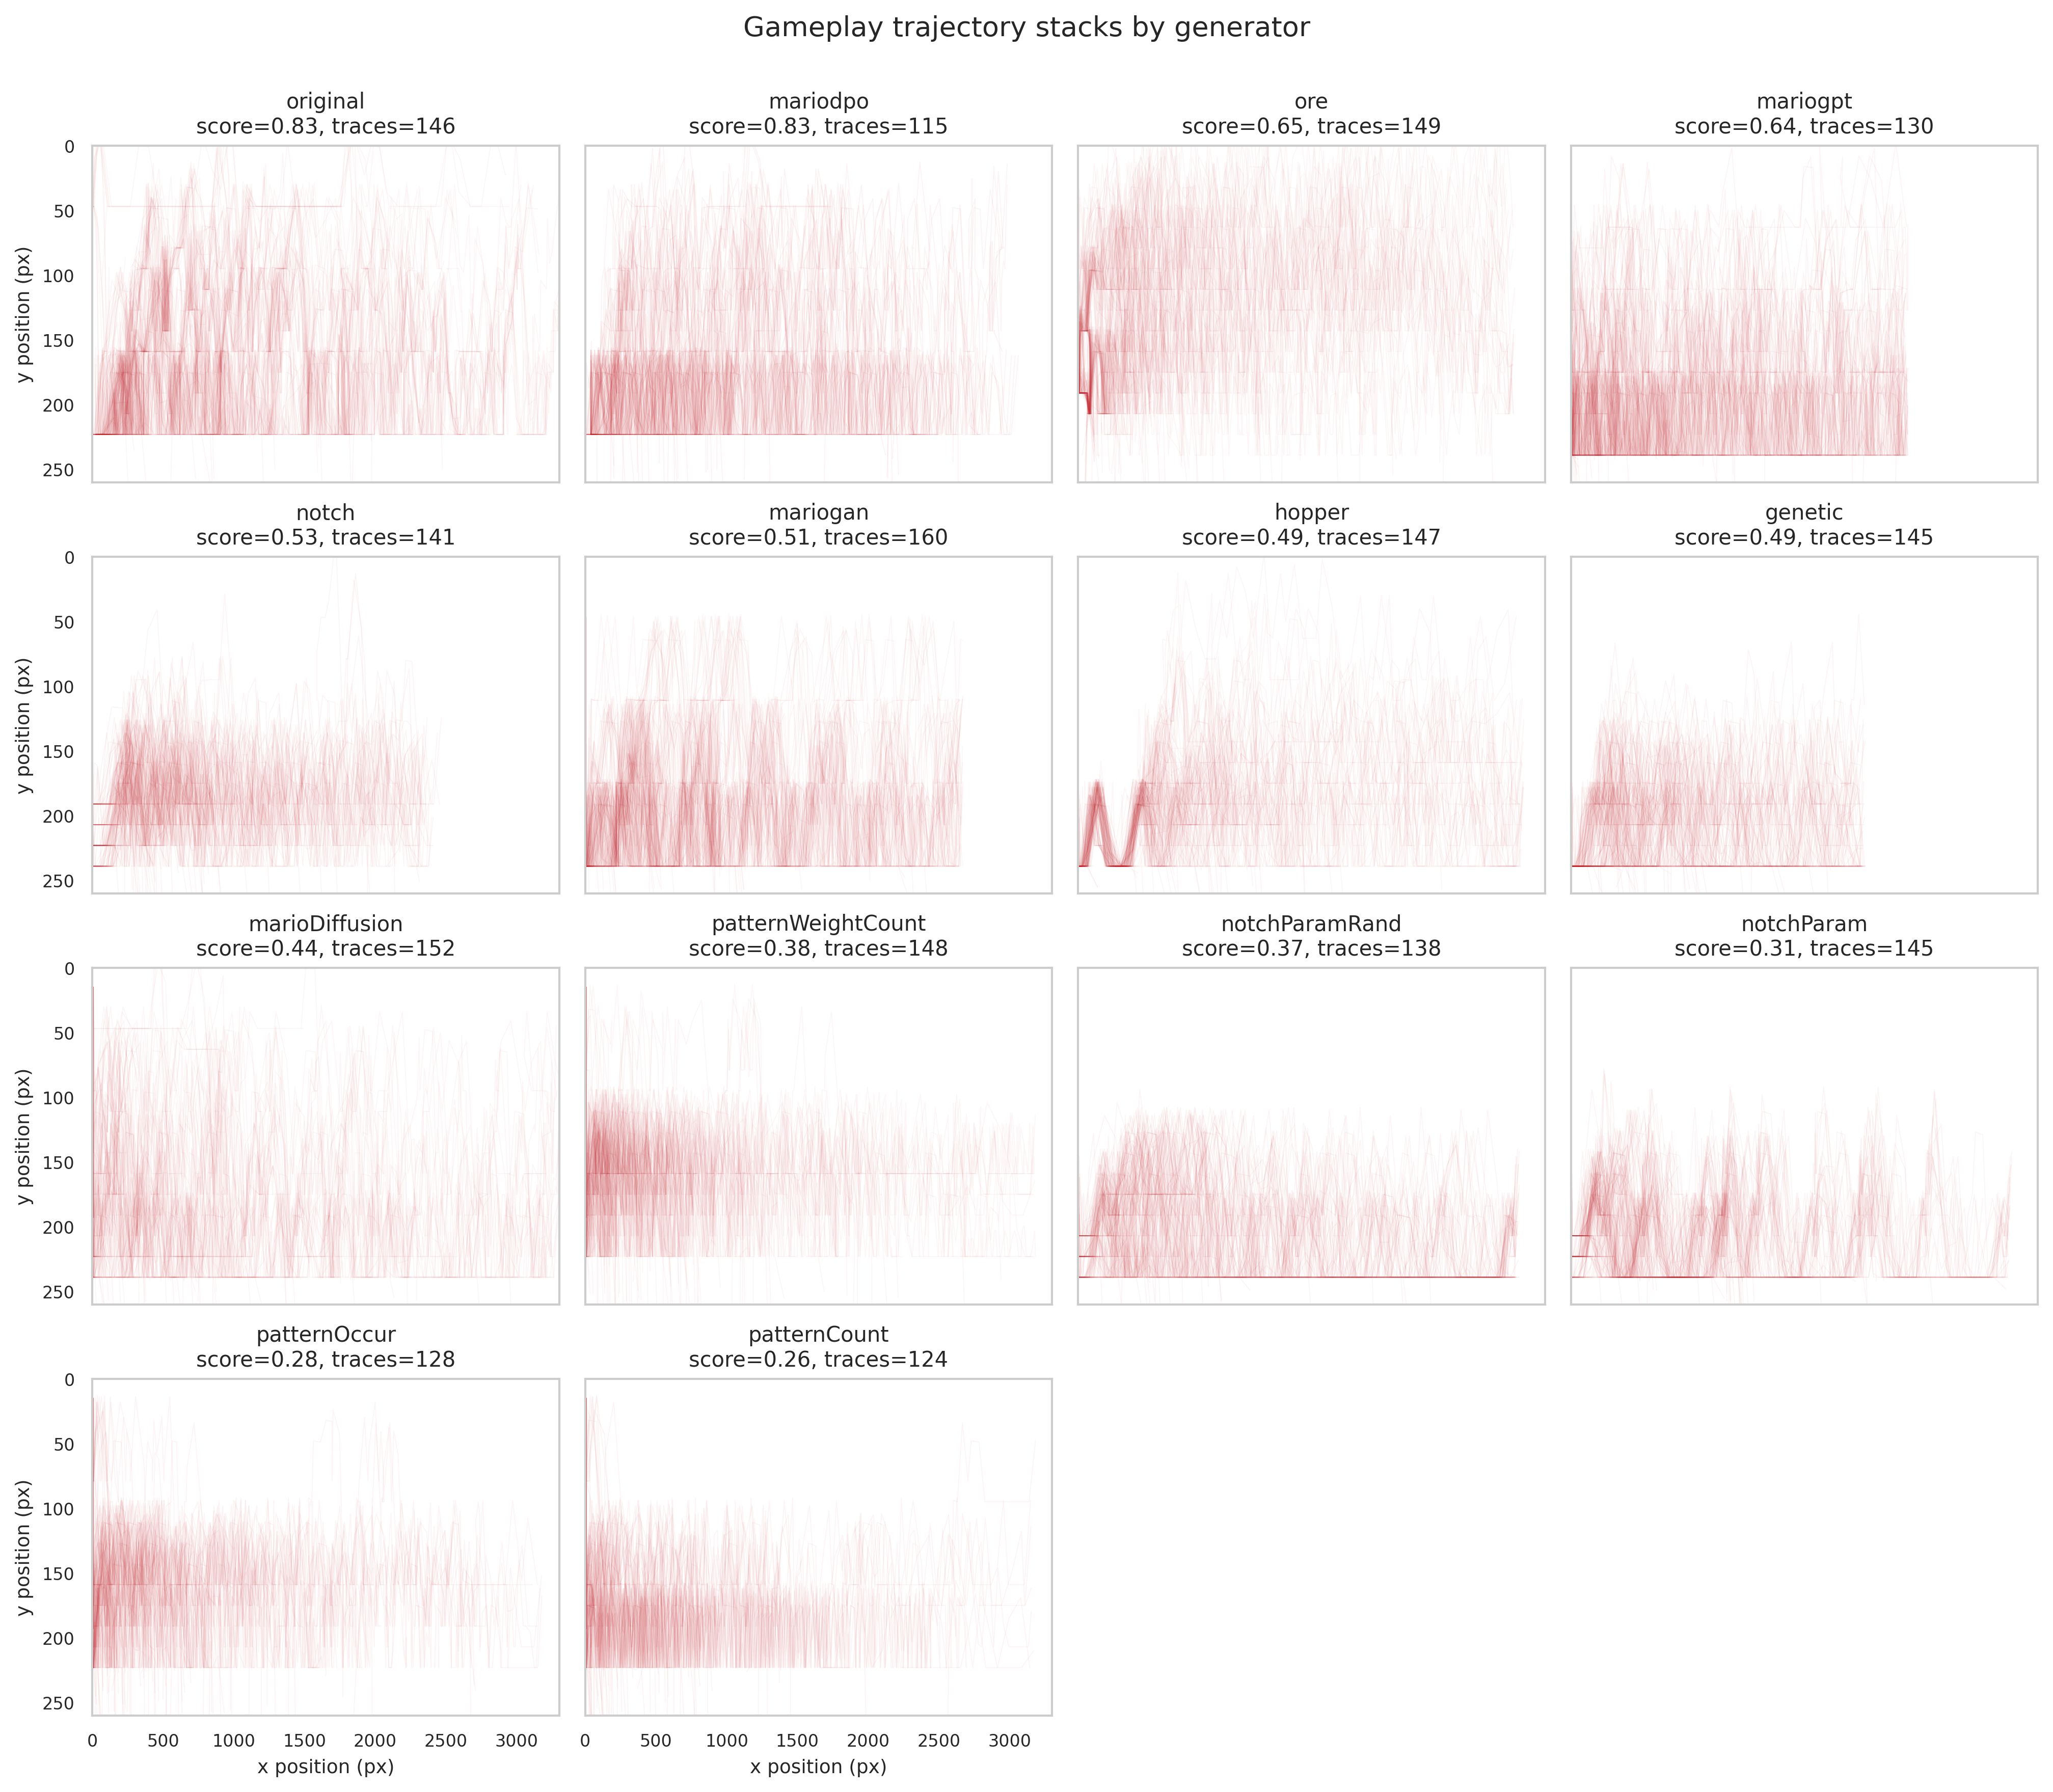
\includegraphics[width=\textwidth]{eda_trajectory_stacks.png}
\caption{Stacked gameplay trajectories by generator. Each subplot overlays all recorded trajectories for one generator as thin red traces on a white background, ordered by preference score. The vertical axis is inverted to match screen coordinates.}
\label{fig:eda-trajectory-stacks}
\end{figure}

The trajectory stacks make generator differences visually apparent. Stronger generators such as \texttt{original} and \texttt{mariodpo} show paths that often progress substantially through the level and occupy a broad portion of the play space. Several low-ranked pattern generators show many traces terminating early or concentrating in narrow regions, consistent with the high early-failure rates computed from death locations.

Figure~\ref{fig:eda-trajectory-metrics} reduces these visual patterns to generator-level summaries. Occupancy entropy measures how broadly trajectories cover a fixed spatial grid. Median maximum $x$ measures progress through the level. Verticality is the mean within-trajectory standard deviation of $y$. Death concentration is the largest share of death locations falling into a single horizontal bin. These are behavioral descriptors of a one-attempt protocol: death-location metrics indicate where failures happen, not how often players retry the same level.

\begin{figure}[H]
\centering
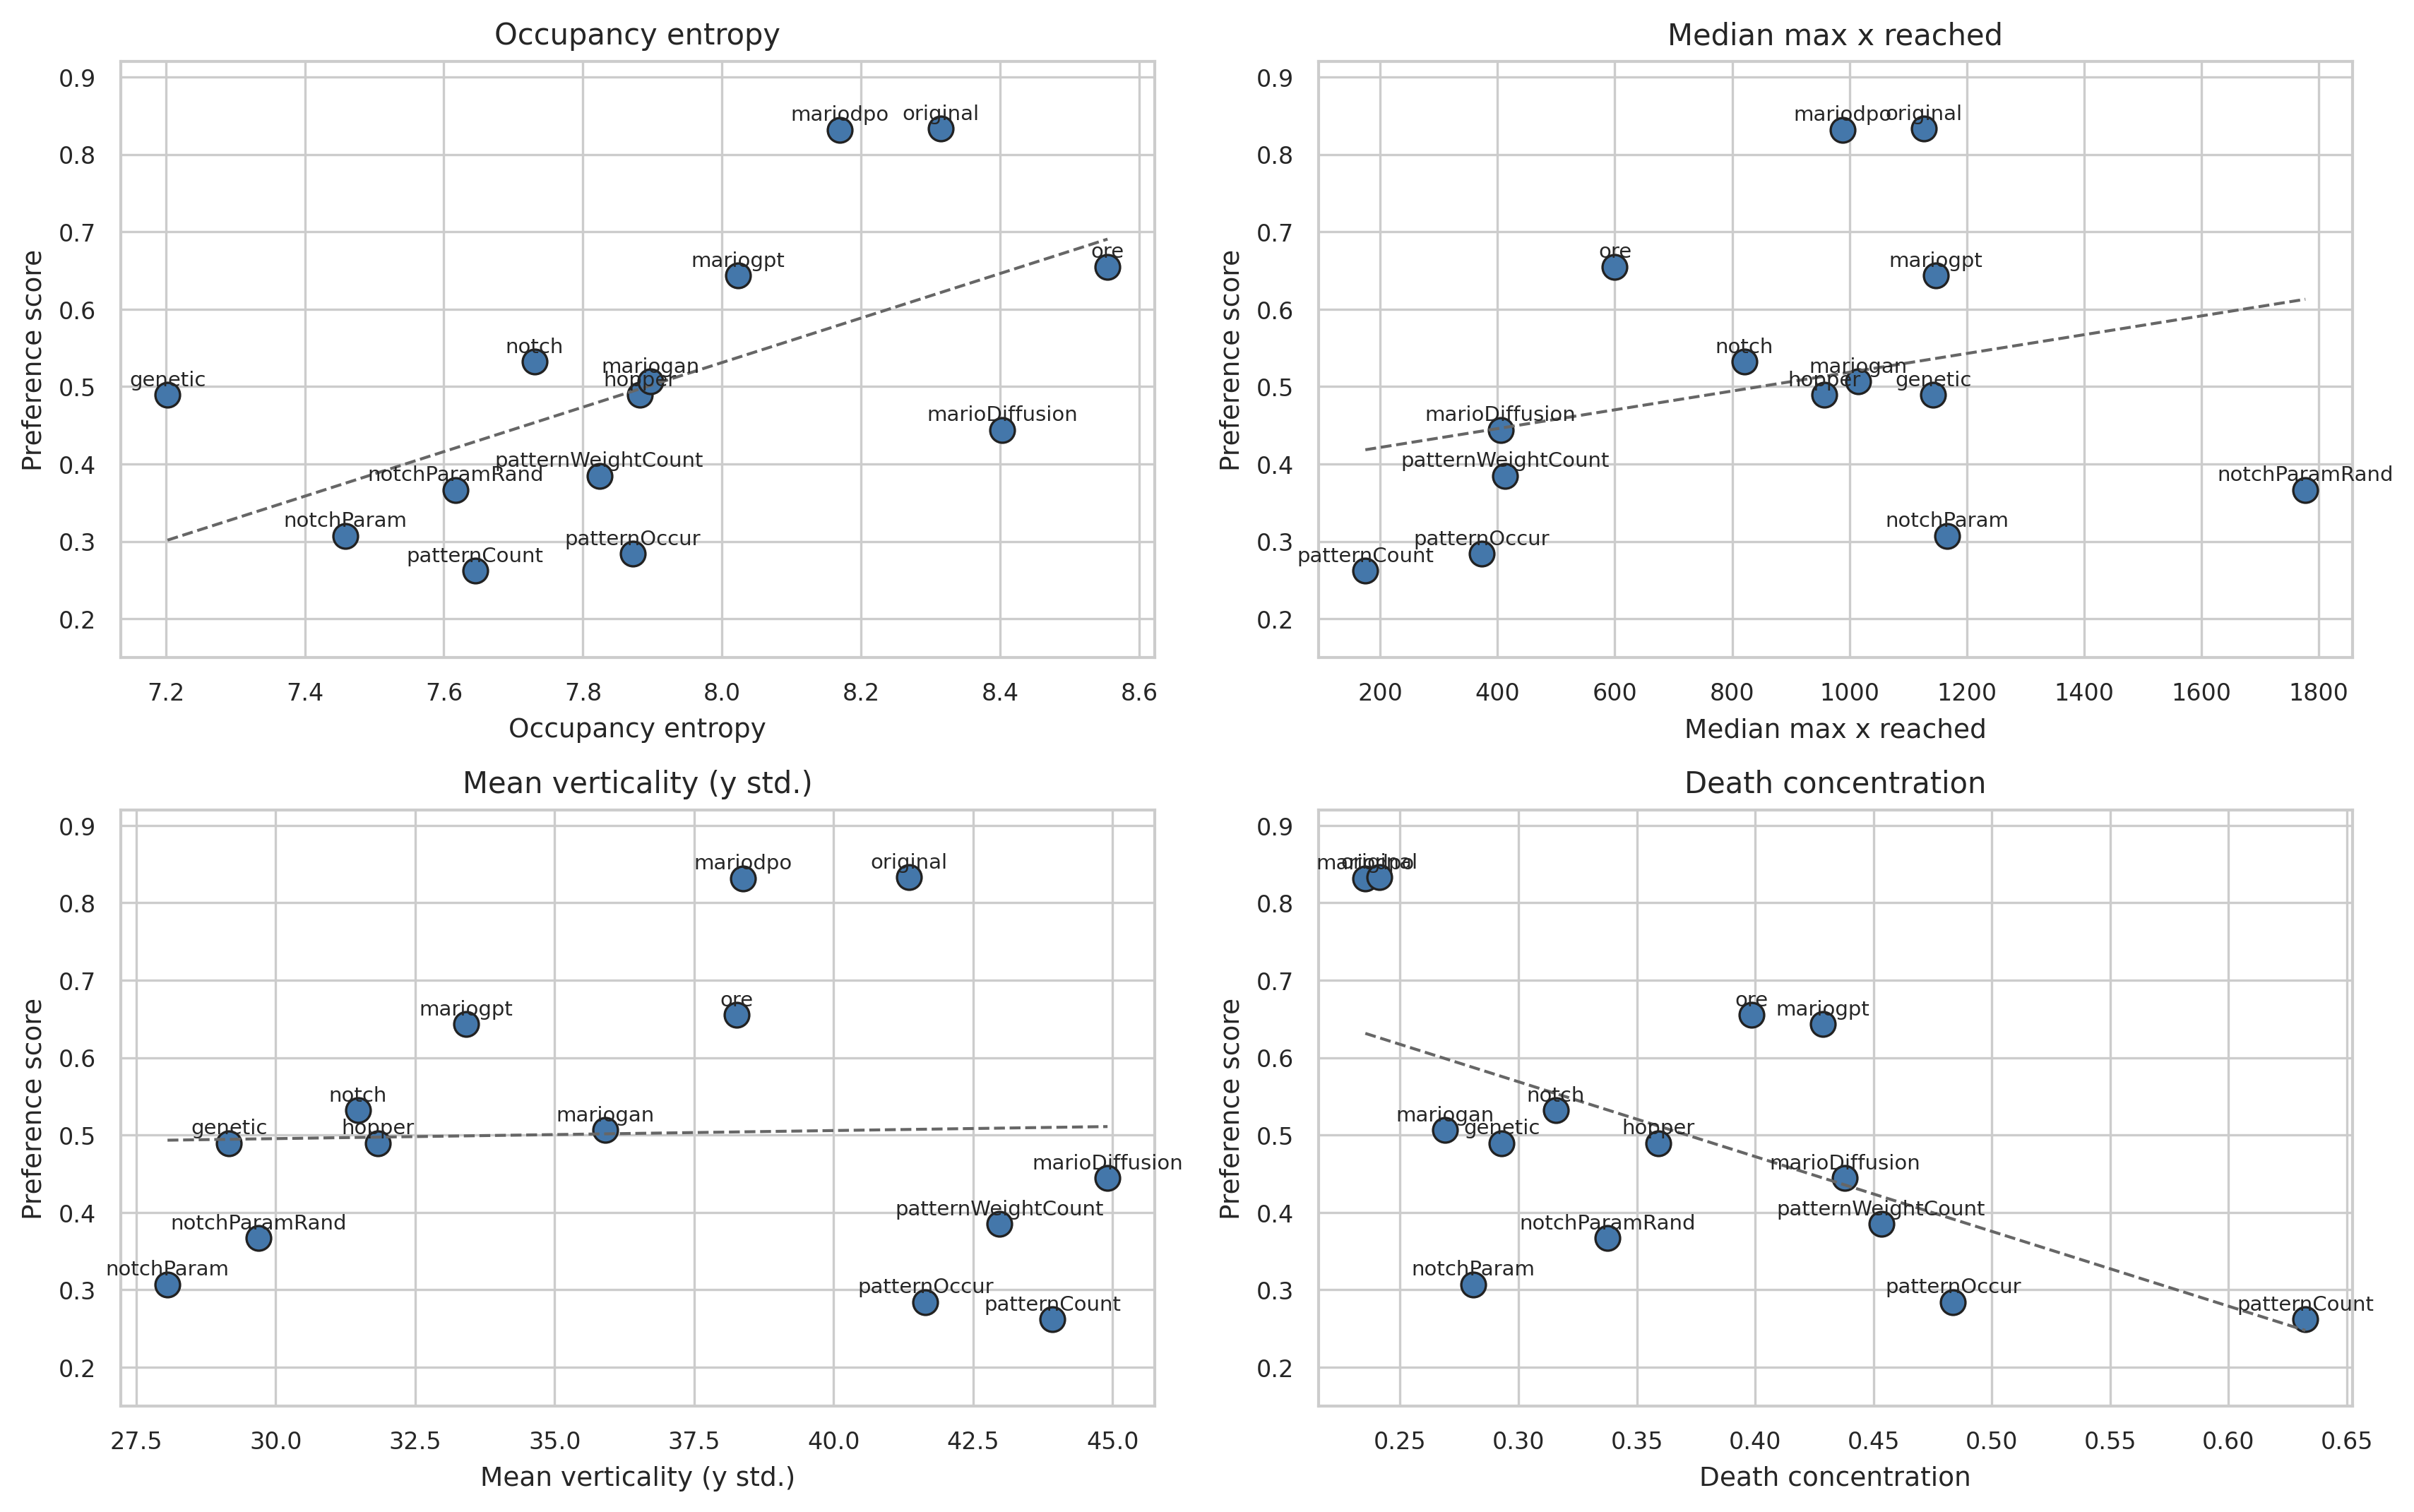
\includegraphics[width=0.95\textwidth]{eda_trajectory_metrics_vs_rating.png}
\caption{Trajectory-derived behavioral summaries versus generator preference score. Higher occupancy entropy and lower death concentration are associated with stronger generators in this export.}
\label{fig:eda-trajectory-metrics}
\end{figure}

The strongest trajectory-level patterns are occupancy entropy and death concentration. Generator-level occupancy entropy has a positive rank association with preference score, while concentrated death locations have a negative association. The weakest pattern generator, \texttt{patternCount}, has median maximum progress of only 174.5 pixels and a max death-bin share of 0.63, meaning failures are highly concentrated early in the level. In contrast, \texttt{original} and \texttt{mariodpo} have median progress around 1126.5 and 988.0 pixels respectively, with lower death concentration.

The deployed analytics UI also supports level-level inspection beyond aggregate plots. Figure~\ref{fig:eda-detailed-level-stats} shows the Detailed Level Statistics page, which combines the level view, player traces, death locations, and tag counts. This is important as a platform contribution: PCG Arena is not only a leaderboard, but also an instrument for diagnosing why a generator wins or loses.

\begin{figure}[H]
\centering
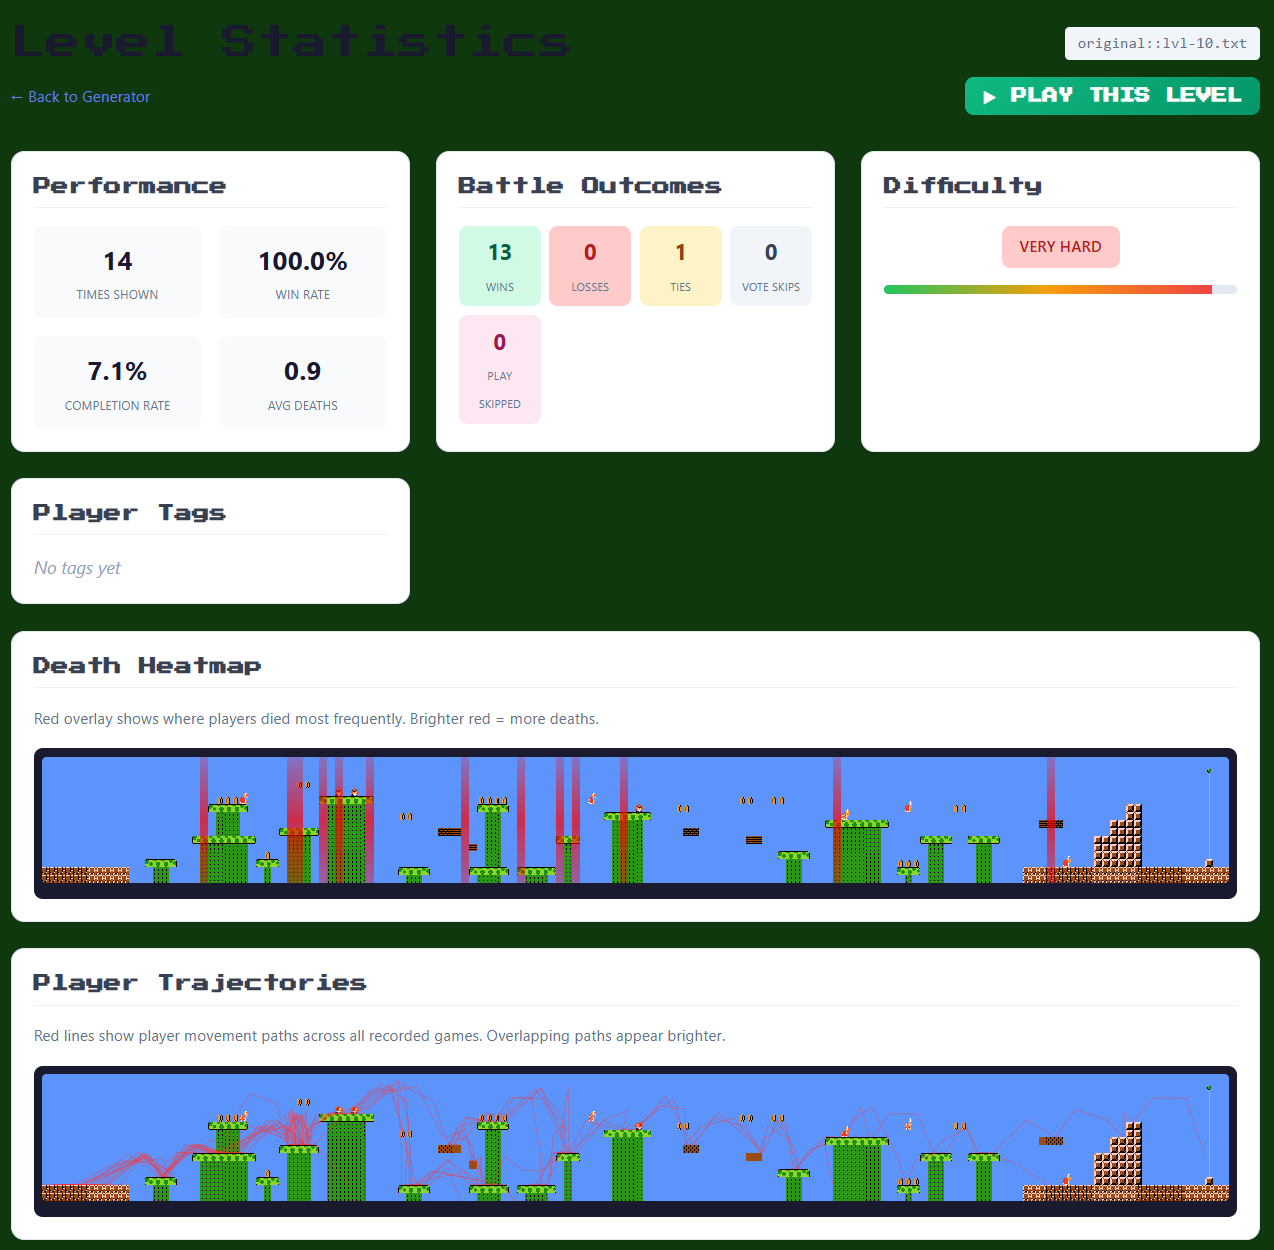
\includegraphics[width=0.95\textwidth]{detailed_level_statistics_page.png}
\caption{Detailed Level Statistics page from PCG Arena. The interface supports qualitative inspection of individual levels through trajectory overlays, death locations, tag counts, and level visualization.}
\label{fig:eda-detailed-level-stats}
\end{figure}

% ===================================================================
\section{RQ4: User Preference Heterogeneity}
\label{sec:eda-user-heterogeneity}

The anonymous-player data are sparse, and because players are identified only by browser/player IDs we know nothing about who they are---their age, background, or gaming experience are all unknown. The data are nonetheless useful for understanding engagement and possible preference heterogeneity. Figure~\ref{fig:eda-engagement} shows votes over time, votes per anonymous player ID, and cumulative vote contribution.

\begin{figure}[H]
\centering
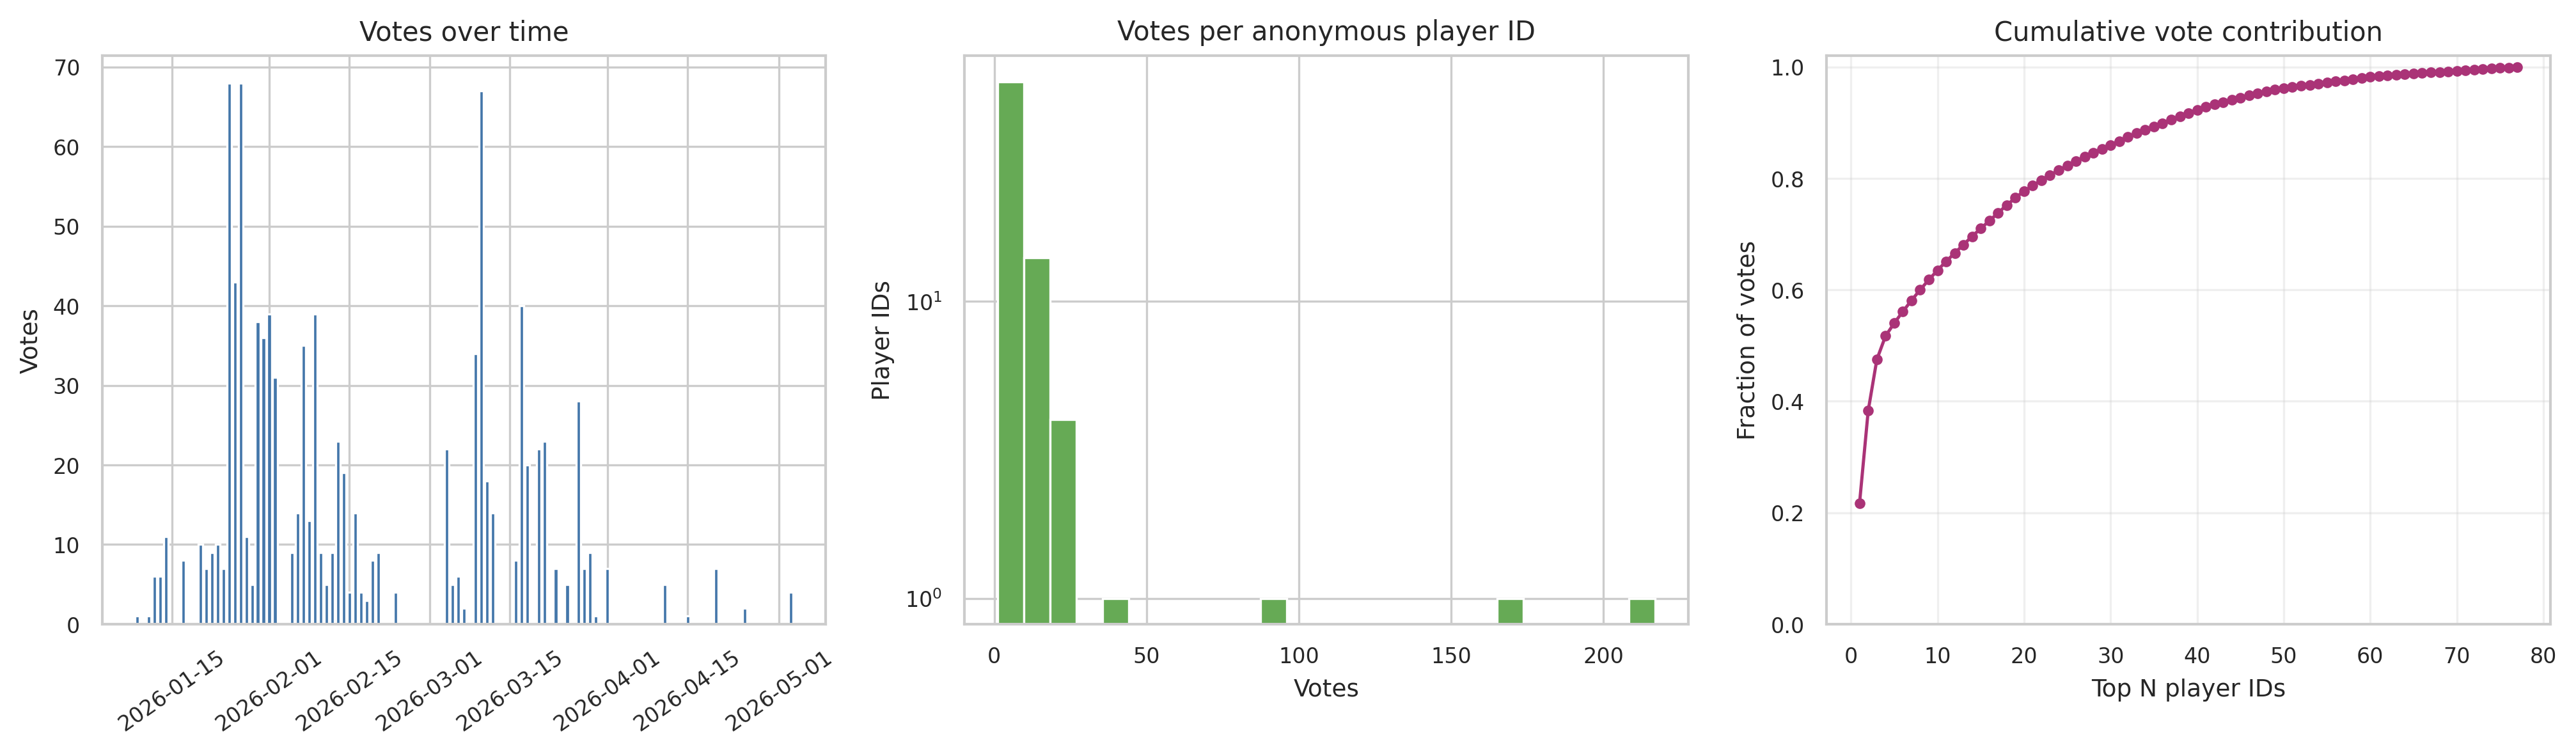
\includegraphics[width=\textwidth]{eda_engagement.png}
\caption{Engagement concentration in the anonymous player-ID data. The analysis uses browser/player IDs, so these counts should not be interpreted as verified unique humans.}
\label{fig:eda-engagement}
\end{figure}

The vote distribution is highly concentrated. Among the 77 anonymous player IDs appearing in the vote table, the median player ID contributes 6 votes, while the most active ID contributes 217 votes. The top 5 IDs account for 54\% of the analyzed votes, and the top 10 account for 63.5\%. This concentration is typical for voluntary web studies, but it matters for interpretation: aggregate generator scores reflect both broad participation and the preferences of a small number of highly engaged player IDs.

Figure~\ref{fig:eda-user-heatmap} examines the player-by-generator preference matrix for anonymous player IDs with at least five votes. Each cell is the mean score assigned by a player ID when that generator appeared. Missing player-generator combinations are filled with the neutral value 0.5 only for visualization and clustering.

\begin{figure}[H]
\centering
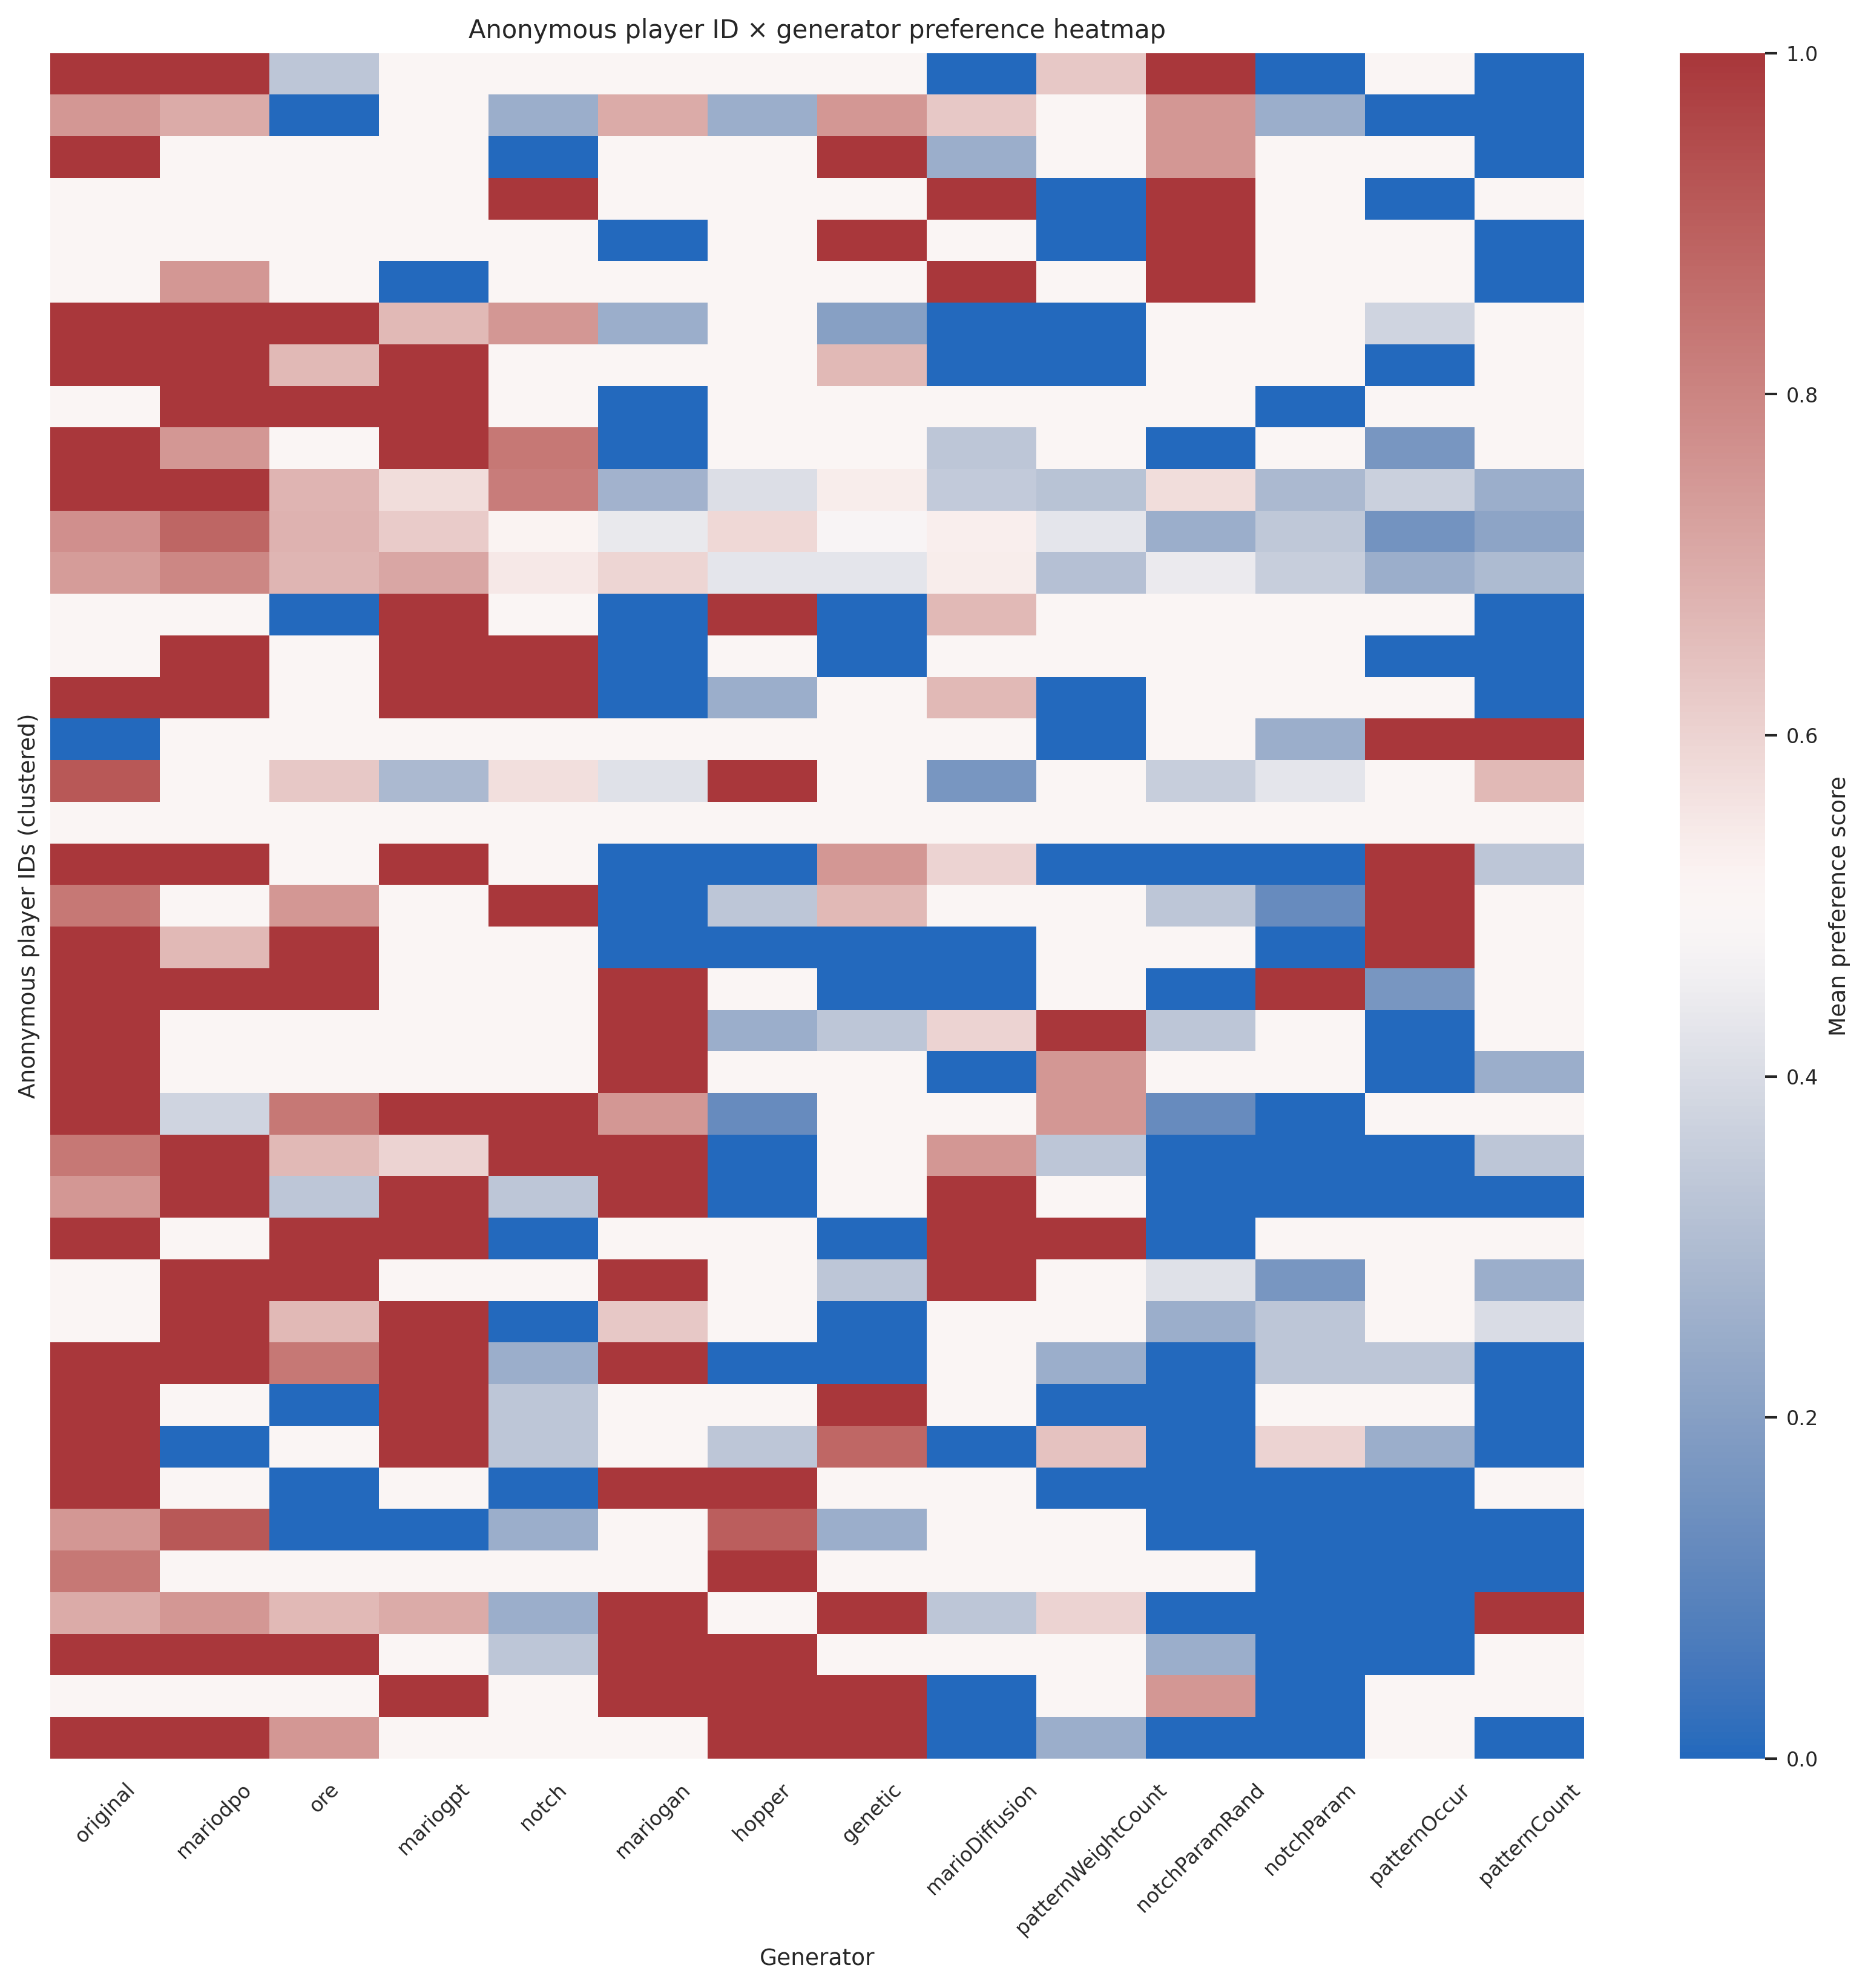
\includegraphics[width=\textwidth]{eda_user_generator_heatmap.png}
\caption{Anonymous player ID by generator preference heatmap for player IDs with at least five votes. Rows are grouped by hierarchical clustering - Ward's method on Euclidean distances between players' generator-score vectors. Columns follow the global generator ranking. The plot is exploratory because many player-generator combinations are sparse.}
\label{fig:eda-user-heatmap}
\end{figure}

The heatmap suggests that, despite some variation, players largely agree on
which generators are good and which are bad: most rows score the top-ranked
generators highly and the bottom-ranked generators poorly, with only mild
disagreement on the mid-table generators. This consistency across an anonymous
and otherwise undescribed player population is itself a useful finding: it
suggests that Super Mario Bros is a strong benchmark for PCG evaluation,
because player preferences over levels are stable enough to produce a
repeatable ranking rather than being dominated by individual taste.

% ===================================================================
\section{RQ5: Tag Semantics and Failure Modes}
\label{sec:eda-tag-semantics}

Tags provide a lightweight qualitative layer over the binary vote. They are optional, sparse, and subjective, so they should not be treated as ground-truth labels. Their value is diagnostic: they help distinguish why a level wins or loses.

Figure~\ref{fig:eda-tag-semantics} summarizes tag frequency, tag rate by generator, tag co-occurrence, and outcome distribution when each tag is present. The most common tags are \texttt{impossible} (87 assignments), \texttt{fun} (56), \texttt{too\_hard} (55), \texttt{boring} (49), \texttt{creative} (39), \texttt{broken\_graphics} (22), and \texttt{too\_easy} (21).

\begin{figure}[H]
\centering
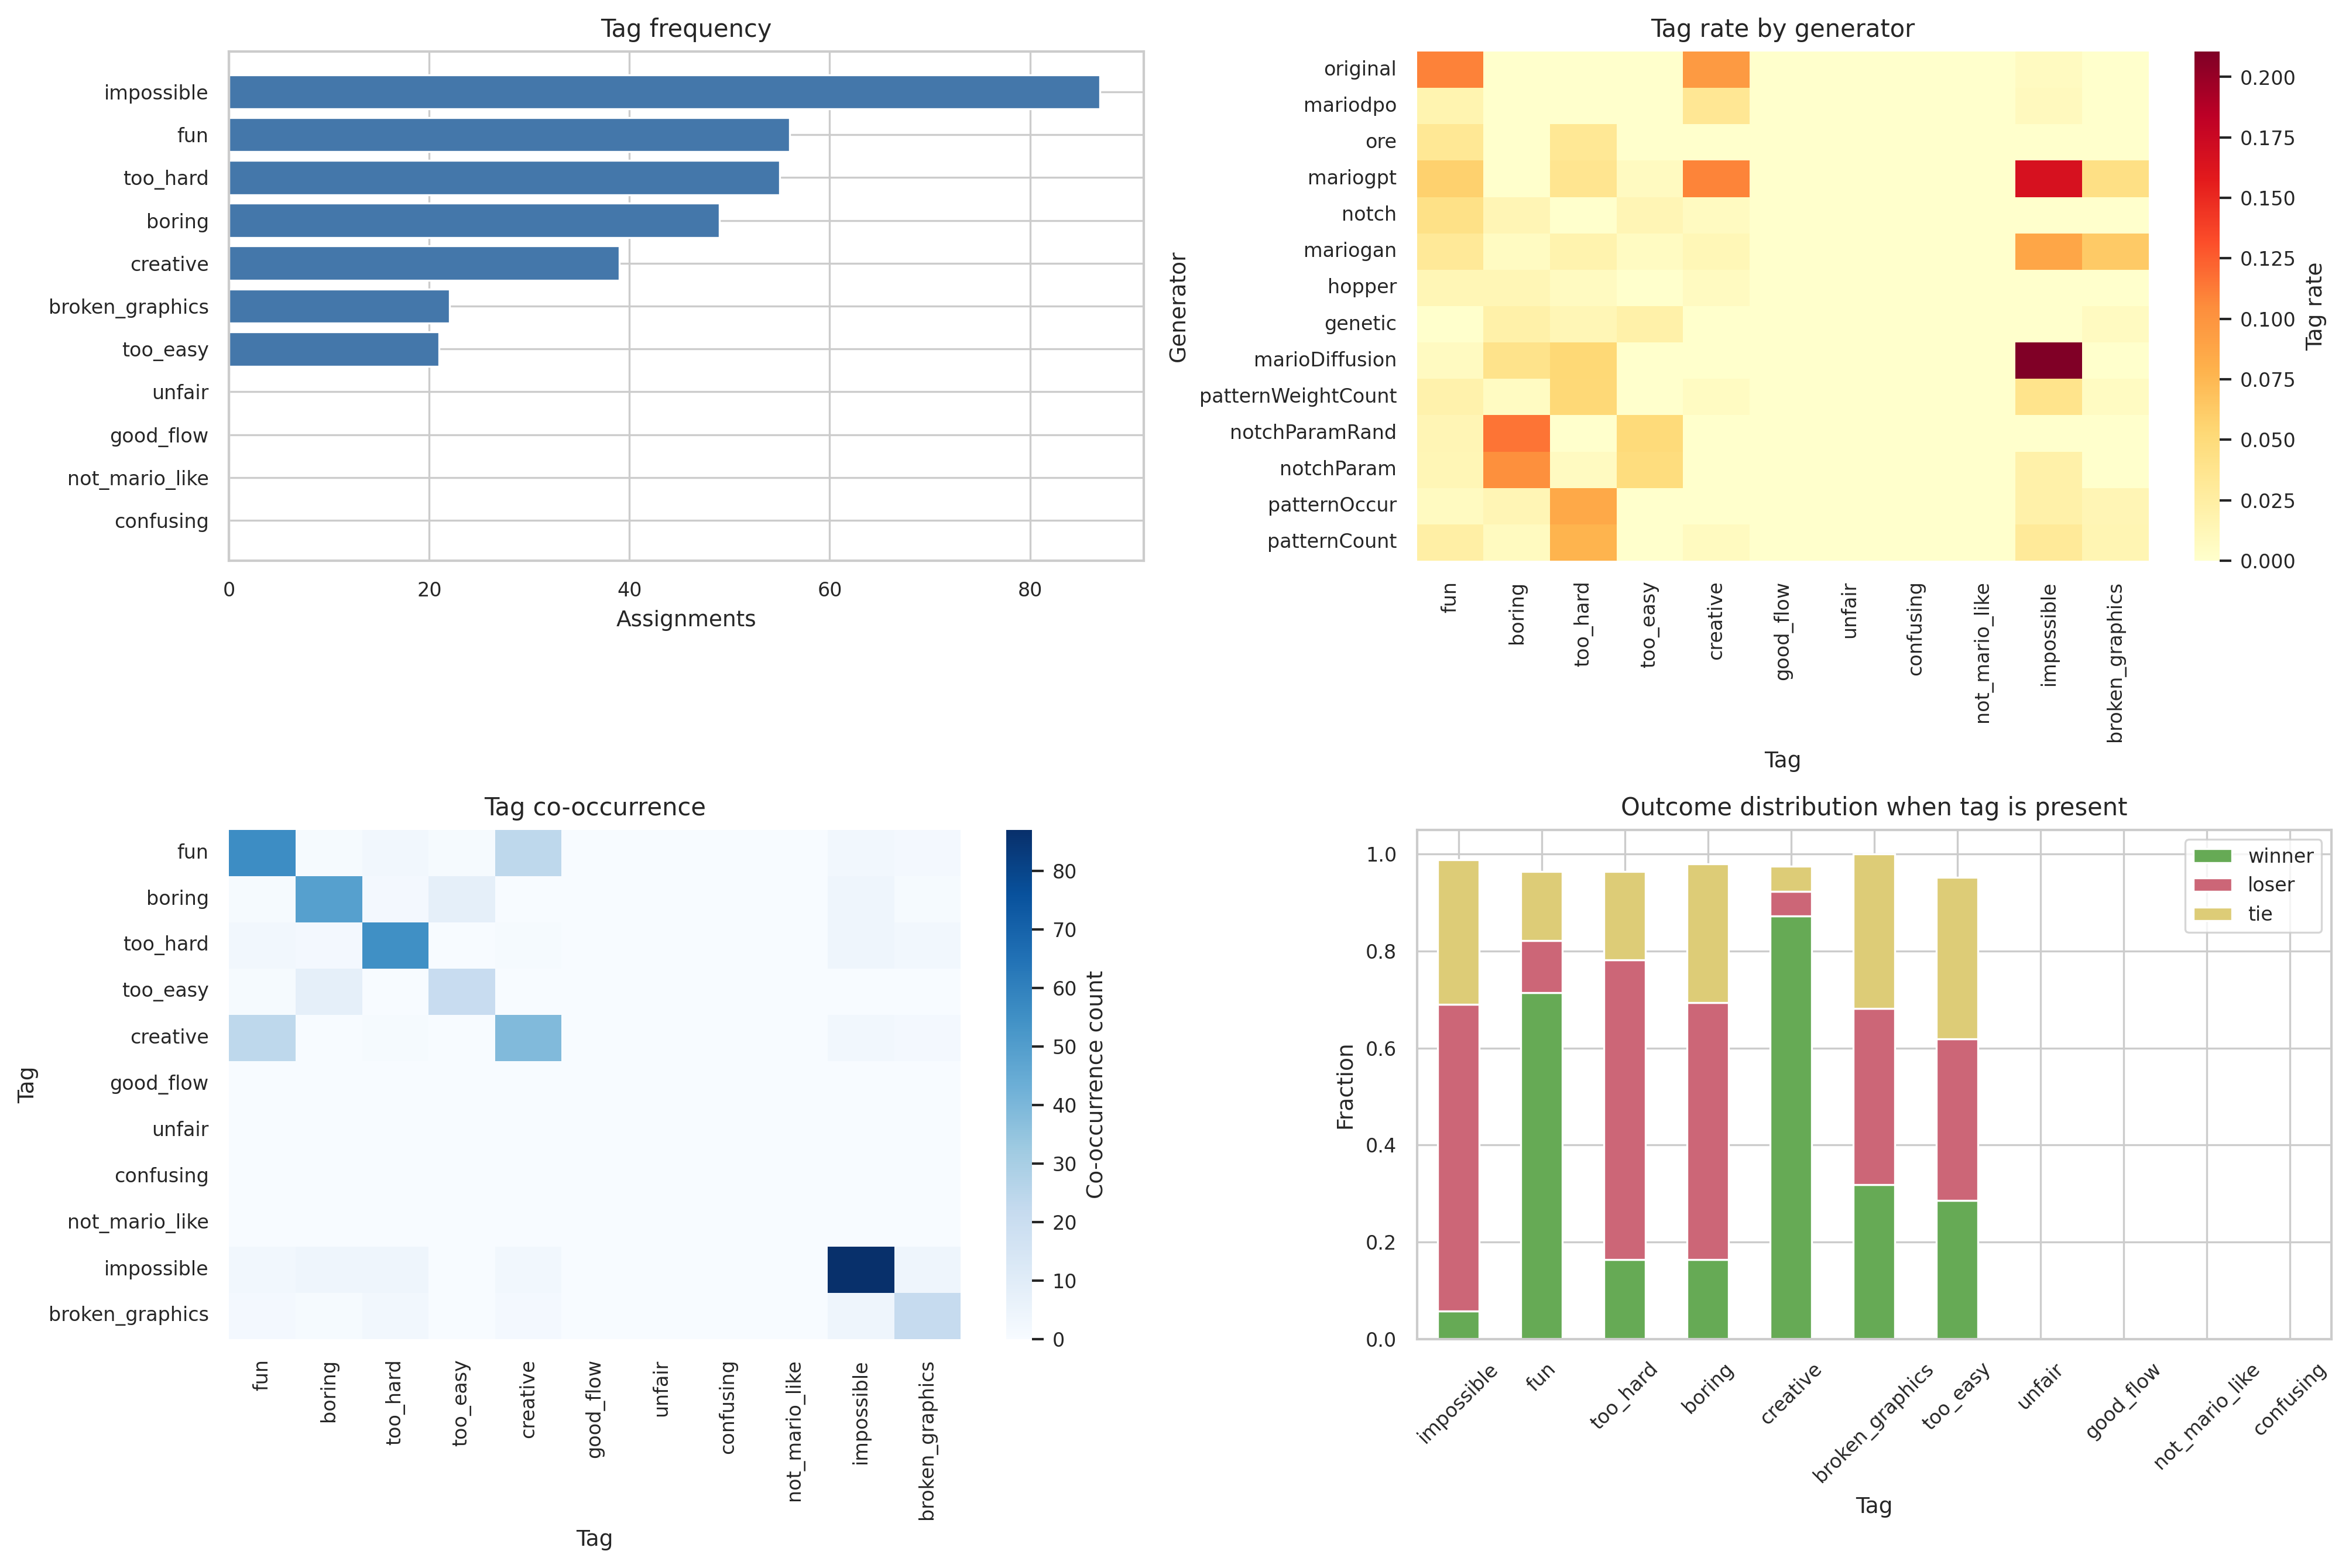
\includegraphics[width=\textwidth]{eda_tag_semantics.png}
\caption{Tag semantics summary. The panels show tag frequency, tag rate by generator, tag co-occurrence, and the outcome distribution for tagged sides.}
\label{fig:eda-tag-semantics}
\end{figure}

Positive tags are strongly aligned with preference outcomes. Sides tagged \texttt{creative} win 87\% of the time and sides tagged \texttt{fun} win 71\% of the time. Negative tags behave differently: \texttt{impossible}, \texttt{too\_hard}, and \texttt{boring} are much more common on losing sides than winning sides. The tag-by-generator heatmap also makes generator failure modes interpretable: some generators lose because they are marked as impossible or too hard, while others are rejected as boring or visually broken.

% ===================================================================
\section{Summary of Findings}
\label{sec:eda-summary}

PCG Arena provides a live human-preference measurement instrument for procedural level generators. It ranks generators through blind pairwise comparison, shows stable head-to-head patterns, connects rankings to static expressive range, reveals behavioral differences through trajectories, exposes engagement concentration and possible preference diversity, and uses tags to explain qualitative failure modes.

The main empirical findings are:
\begin{enumerate}[nosep]
    \item \textbf{Preference ranking}: \texttt{original} and \texttt{mariodpo} are the top generators in the analyzed export, with nearly identical preference scores around 0.83.
    \item \textbf{Generator families}: Pattern-based generators are consistently weak, while neural and constructive generators occupy the middle tiers.
    \item \textbf{Static structure}: Generators occupy visibly distinct expressive ranges. Reward density, unique-column ratio, and distance to the original corpus are more informative than any single difficulty proxy.
    \item \textbf{Gameplay behavior}: Trajectories reveal navigability and failure modes. Stronger generators tend to support broader movement footprints and less concentrated failure locations.
    \item \textbf{Users}: Player votes are largely consistent across the anonymous population: the same generators tend to score high or low across players, suggesting that Super Mario Bros is a good benchmark whose preference signal is not dominated by individual taste.
    \item \textbf{Tags}: Optional tags add semantic explanations to votes, distinguishing positive qualities such as \texttt{fun} and \texttt{creative} from failure modes such as \texttt{impossible}, \texttt{too\_hard}, and \texttt{boring}.
\end{enumerate}

These findings directly inform the design of the preference-aligned generation pipeline described in the following chapter.


\chapter{MarioDPO --- Preference-Aligned Level Generation}
\label{ch:mariodpo}


\section{Motivation and Overview}
\label{sec:dpo-motivation}

The exploratory analysis of Chapter~\ref{ch:eda} established three facts that
motivate the final contribution of this thesis. Blind pairwise votes produce a
stable ranking in which the hand-authored original levels lead; player preference
is multi-dimensional, so no single automated metric reproduces that ranking on
its own; yet the votes themselves constitute a large, reusable training signal.
MarioDPO uses this signal not merely to \emph{rank} generators, but to
\emph{train} one, closing the loop from human evaluation back to generation.

The method has three stages. First, a \emph{judge function} learns to predict,
from a level's tiles alone, which of two levels a player would prefer; this turns
a few hundred sparse votes into a scorer that can be applied to any freshly
generated level. Second, a pretrained Mario language model is
\emph{continue-pretrained} on the arena level corpus so that it speaks the
platform's exact $16$-row, $37$-tile representation. Third, the model is aligned
with \emph{Direct Preference Optimisation} (DPO; Section~\ref{subsec:bg-dpo}) on
the human votes, augmented by additional pairs that the judge labels
automatically.

A deliberate design principle separates \textbf{validity} from
\textbf{preference}. Validity---a safe spawn, a reachable flag, solid ground at
the boundaries, only legal tiles---is guaranteed by the representation and a
deterministic post-processing pass. Preference---whether the level is actually
enjoyable---is what the judge and DPO optimise. Levels are serialised
\emph{column-major} (one $16$-character column at a time) so that vertically
adjacent tiles stay adjacent in the token stream, and wide levels are handled
with a sliding window, as described in Section~\ref{subsec:bg-pcgml}. The learned
model can therefore concentrate on quality while hard constraints are enforced
outside it.

\section{The Judge Function}
\label{sec:dpo-judge}

Human votes are the most trustworthy signal on the platform, but far too sparse
to train a sequence model directly. The judge function bridges this gap: it is a
lightweight scorer $J(\ell)\in\mathbb{R}$ that estimates the human-preferred-ness
of a level $\ell$ from \emph{static structural features only}---tile densities,
gap statistics, surface linearity, reward content, diversity, and compression
distance to the original corpus. It deliberately uses neither gameplay telemetry
nor the identity of the generator, so it can score a never-before-seen generated
level and cannot ``cheat'' by recognising which system produced a level.

The judge is trained on antisymmetric feature \emph{differences}: each non-tie
vote contributes a pair $(\ell_w,\ell_l)$, and the model learns that
$f(\ell_w)-f(\ell_l)$ maps to ``win'' and its negation to ``loss''. We hold out
$10\%$ of votes---split by vote, so no level appears in both folds---and select
among four candidate scorers (an interpretable hand-weighted heuristic, a linear
Bradley--Terry model, gradient boosting, and a small MLP) by held-out pairwise
AUC. Table~\ref{tab:dpo-judge-candidates} reports the comparison.

\begin{table}[H]
\centering
\caption{Judge candidates on a held-out $10\%$ split of votes (split by vote).
The linear Bradley--Terry model is selected for its best held-out AUC and its
interpretability. ``Gen.\ Spearman'' correlates each candidate's per-generator
mean score with the empirical arena win rate.}
\label{tab:dpo-judge-candidates}
\begin{tabular}{lccc}
\toprule
\textbf{Candidate} & \textbf{Held-out acc.} & \textbf{Held-out AUC} & \textbf{Gen.\ Spearman} \\
\midrule
Hand-weighted heuristic        & 0.610 & 0.635 & 0.411 \\
\textbf{Linear Bradley--Terry} & 0.720 & \textbf{0.809} & 0.965 \\
Gradient boosting              & 0.744 & 0.799 & 0.982 \\
MLP                            & 0.732 & 0.795 & 0.991 \\
\bottomrule
\end{tabular}
\end{table}

The linear Bradley--Terry judge is selected: it attains the best held-out AUC
($0.809$) while remaining fully interpretable, and it generalises better than the
nonlinear models, which fit the training pairs more tightly (gradient boosting
reaches $0.905$ training accuracy) without improving held-out ranking. As an
external check, aggregating its per-level scores by generator and correlating the
result with the empirical arena win rate gives a Spearman $r_s = 0.965$: a scorer
trained only on pairwise tile differences recovers almost the entire human
leaderboard. Figure~\ref{fig:dpo-judge-validation} shows both the learned weights
and this generator-level agreement.

\begin{figure}[H]
\centering
\begin{subfigure}{0.49\textwidth}
\centering
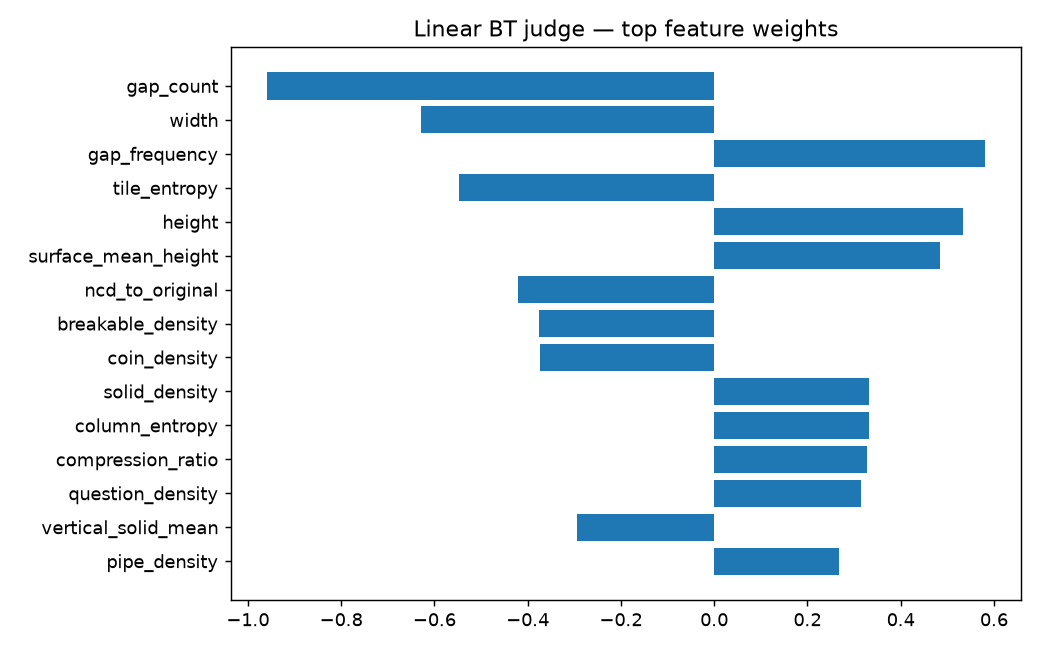
\includegraphics[width=\textwidth]{mariodpo_judge_weights.png}
\caption{Learned feature weights.}
\label{fig:dpo-judge-weights}
\end{subfigure}
\hfill
\begin{subfigure}{0.49\textwidth}
\centering
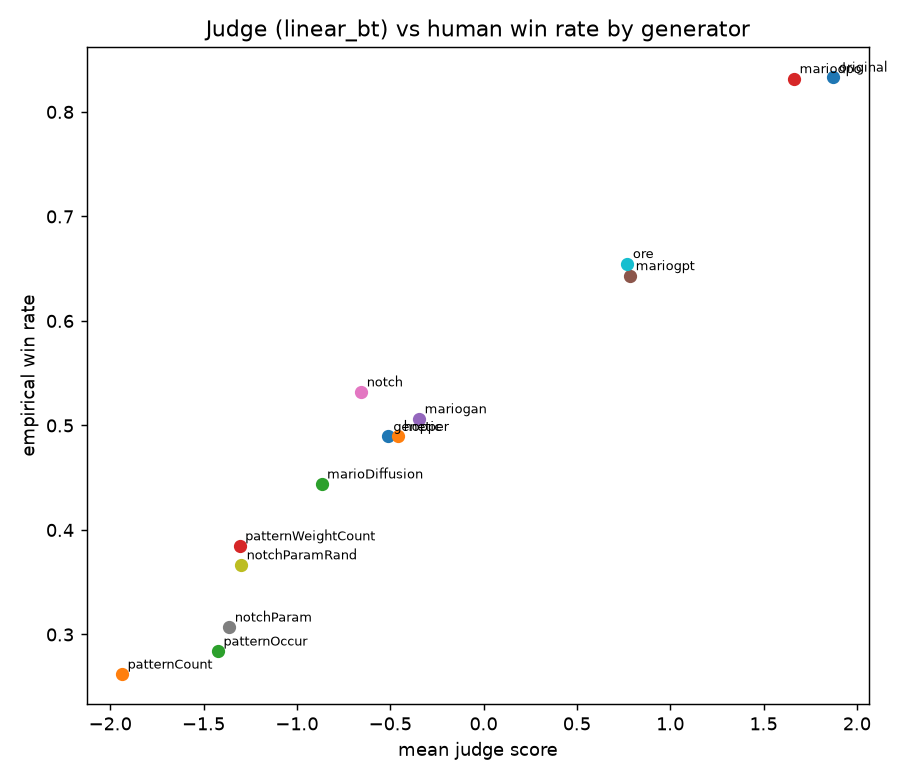
\includegraphics[width=\textwidth]{mariodpo_judge_winrate.png}
\caption{Judge score vs.\ arena win rate.}
\label{fig:dpo-judge-winrate}
\end{subfigure}
\caption{Judge-function validation. (a)~The linear Bradley--Terry judge penalises
gaps and excess width while rewarding structural variety and reward content.
(b)~Aggregated per generator, the judge score tracks the empirical human win rate
($r_s = 0.965$), recovering almost the entire arena leaderboard from static
features alone.}
\label{fig:dpo-judge-validation}
\end{figure}

The learned weights are legible as design guidance. Large gap counts and
excessive width are penalised most strongly, while structural variety (column
entropy, compression ratio), reward content (question blocks), and a moderate
surface profile are rewarded; distance from the original corpus is penalised.
These are precisely the structural correlates of preference identified
descriptively in Chapter~\ref{ch:eda}, now recovered automatically as the
coefficients of a predictive model.

\section{Generator Training}
\label{sec:dpo-training}

\subsection{Continue-pretraining the base model}
\label{subsec:dpo-sft}

The base policy $\pi_{\mathrm{ref}}$ is the pretrained MarioGPT
checkpoint~\citep{sudhakaran2023mariogpt}, a GPT-2 decoder. It is
continue-pretrained on the arena corpus---every seed level, serialised
column-major into $8{,}521$ overlapping windows, with the original Nintendo
levels upweighted three-fold---under a standard next-token objective; this model
then serves as the reference policy $\pi_{\mathrm{ref}}$ in the DPO objective of
Equation~\ref{eq:dpo}. The stage teaches the model the platform's exact
representation and the syntax of valid levels: ground along the lower rows,
multi-tile pipes, blocks above reachable space, enemies on supports. Three epochs
reduce the loss to $0.26$ in under five minutes on a single $6$\,GB
GPU.\footnote{All training runs are logged publicly to Weights \& Biases at
\url{https://wandb.ai/antoni-krzysztof-czapski/mario-dpo}; the
continue-pretraining run is
\href{https://wandb.ai/antoni-krzysztof-czapski/mario-dpo/runs/fqryf451}{\texttt{sft}}.}

\subsection{Preference dataset}
\label{subsec:dpo-dataset}

DPO consumes triples: a shared prompt, a preferred completion, and a rejected
one. Two sources are combined (Table~\ref{tab:dpo-dataset}). Every non-tie arena
vote becomes a human pair $(\ell_w,\ell_l)$; because these are the only direct
measurements of preference, they are oversampled ten-fold. To broaden coverage,
the judge scores the seed corpus and forms additional synthetic pairs whenever
two levels differ by at least $0.5$ in judge score, which retains only
unambiguous comparisons. The result is $10{,}160$ training records, dominated by
the human votes but enriched with clear judge-labelled negatives.

\begin{table}[H]
\centering
\caption{Preference dataset for DPO fine-tuning. Human votes are oversampled
ten-fold relative to the judge-labelled synthetic pairs.}
\label{tab:dpo-dataset}
\begin{tabular}{lrrr}
\toprule
\textbf{Source} & \textbf{Pairs} & \textbf{Weight} & \textbf{Records} \\
\midrule
Human PCG Arena votes          & 816   & $10\times$ & 8,160 \\
Judge-labelled synthetic pairs & 2,000 & $1\times$  & 2,000 \\
\midrule
\textbf{Total}                 & \textbf{2,816} & --- & \textbf{10,160} \\
\bottomrule
\end{tabular}
\end{table}

\subsection{DPO alignment}
\label{subsec:dpo-align}

Starting from $\pi_{\mathrm{ref}}$, the policy is fine-tuned with the DPO
objective of Equation~\ref{eq:dpo} using a low-rank adapter
(LoRA, $r = 16$, $\alpha = 32$), which holds a single copy of the base weights in
memory and fits comfortably on the $6$\,GB GPU. The penalty $\beta = 0.1$ limits
drift from the reference, and a small learning rate ($10^{-5}$) suits the
preference-rich but modest dataset; Table~\ref{tab:dpo-config} lists the
configuration. Over three epochs the implicit reward accuracy---how often the
policy ranks the preferred level above the rejected one---rises from $0.45$ to
$0.70$, with a reward margin of $0.69$, confirming that the model internalises the
preference signal.\footnote{DPO run:
\href{https://wandb.ai/antoni-krzysztof-czapski/mario-dpo/runs/uo8h2xys}{\texttt{dpo}}.}

\begin{table}[H]
\centering
\caption{MarioDPO training configuration. Both stages run in fp16 on a single
$6$\,GB GPU.}
\label{tab:dpo-config}
\begin{tabular}{ll}
\toprule
\textbf{Stage / parameter} & \textbf{Value} \\
\midrule
Base model            & pretrained MarioGPT (GPT-2 decoder) \\
Representation        & column-major, $16$ rows, $37$ tiles \\
SFT corpus            & $8{,}521$ sliding windows (original $\times 3$) \\
SFT epochs / LR       & $3$ / $5\times10^{-5}$ \\
DPO method            & LoRA ($r{=}16$, $\alpha{=}32$) \\
DPO $\beta$ / LR      & $0.1$ / $10^{-5}$ \\
DPO epochs            & $3$ \\
\bottomrule
\end{tabular}
\end{table}

At inference, preference alignment is combined with the hard validity guarantees.
For each requested level the model samples several candidates, discards any that
fail format checks, scores the rest with the judge, and keeps the best; a
deterministic post-processing pass then guarantees a safe spawn, a reachable
flag, and solid ground at both ends. The learned model supplies \emph{quality};
the filter supplies \emph{validity}.

\section{Results}
\label{sec:dpo-results}

Because fresh human votes cannot be gathered offline, the trained generator is
evaluated in two complementary ways: the validated judge scores its output
against every baseline, and a held-out set of real votes tests whether alignment
moved the policy in the human-preferred direction.

Figure~\ref{fig:dpo-judge-distributions} compares the judge scores of MarioDPO's
levels with the established generators. All generated levels pass validation, and
their mean judge score ($2.64$) is the highest in the field---above the
hand-authored original corpus ($1.87$), the neural baselines MarioGPT and ORE
(both $\approx 0.78$), and far above the pattern-based generators (all negative).
The generator has learned to populate the same high-scoring region of structural
feature space that characterises the most-preferred human levels.

\begin{figure}[H]
\centering
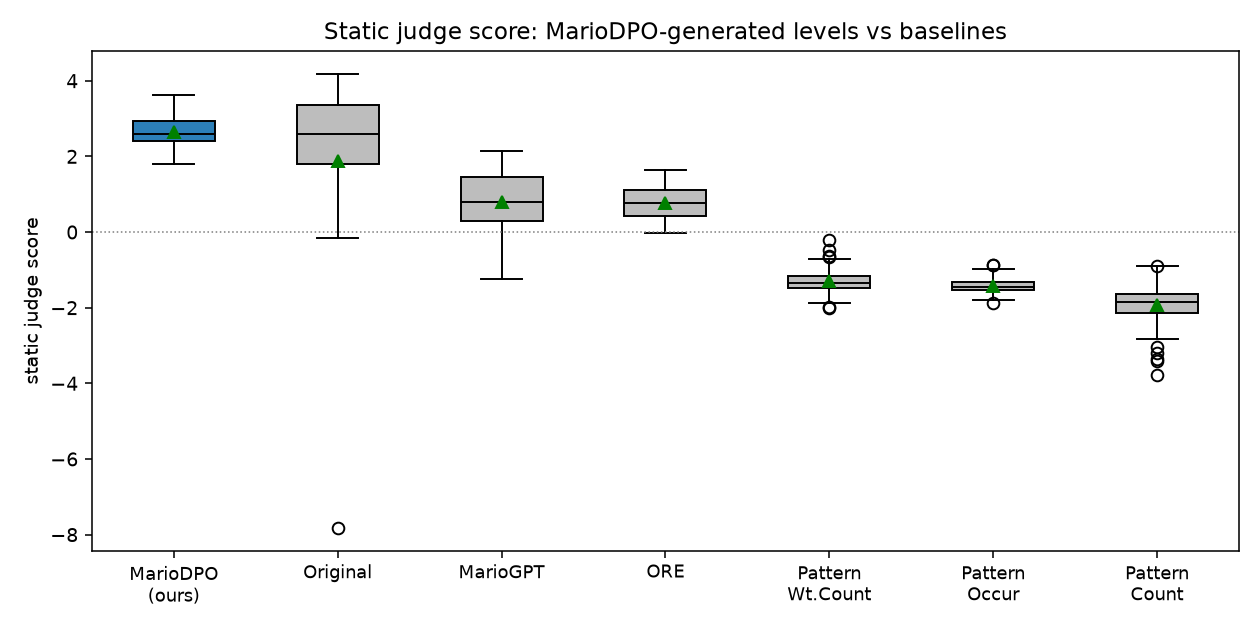
\includegraphics[width=0.95\textwidth]{mariodpo_judge_distributions.png}
\caption{Static judge scores of MarioDPO-generated levels against the baseline
generators (green triangles mark means). The generated levels sit at the top of
the distribution, matching the hand-authored original corpus and clearly
exceeding the other procedural generators.}
\label{fig:dpo-judge-distributions}
\end{figure}

Figure~\ref{fig:dpo-pref-accuracy} reports the second test. On a held-out split
of real votes, the aligned policy assigns higher likelihood to the
human-preferred level more often than its own pre-DPO reference ($0.39$ versus
$0.37$). Both values sit below the $0.5$ chance line---length-normalised sequence
likelihood over a short level window is a deliberately strict and noisy proxy, and
the held-out split is small---so the absolute numbers should not be over-read; the
meaningful quantity is the \emph{direction} of the change, which is positive and
consistent with the training-time reward accuracy of $0.70$.

\begin{figure}[H]
\centering
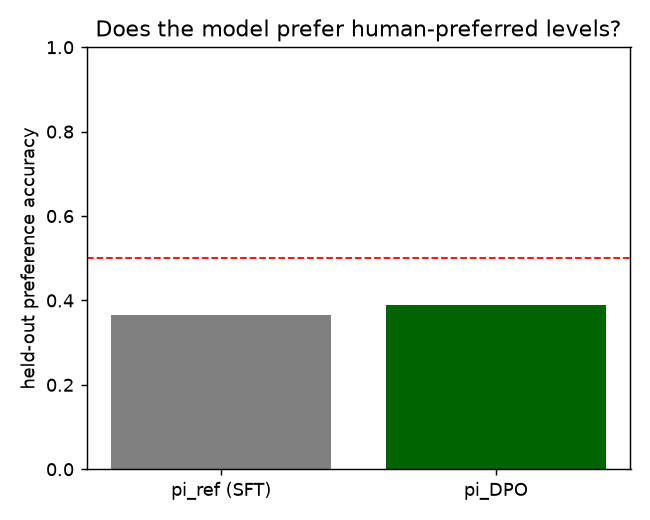
\includegraphics[width=0.6\textwidth]{mariodpo_preference_accuracy.png}
\caption{Held-out preference accuracy: how often each policy assigns higher
likelihood to the human-preferred level. DPO improves over its SFT reference; the
dashed line marks chance. Absolute values are modest because length-normalised
sequence likelihood over a short window is a strict proxy on a small split.}
\label{fig:dpo-pref-accuracy}
\end{figure}

Finally, the generator was deployed on the live platform and evaluated under the
same blind protocol as every other system. In the arena export analysed in
Chapter~\ref{ch:eda}, MarioDPO attains a preference score of $0.832$, essentially
tied with the original Nintendo levels ($0.833$) and ahead of every other
procedural generator. The offline judge improvement and the online human result
agree: preference alignment lifts the generator into the same top tier as the
hand-authored baseline.

\section{Discussion}
\label{sec:dpo-discussion}

Three design choices explain the outcome. The model begins from a strong prior,
so DPO spends its capacity improving quality rather than rediscovering basic level
syntax. The judge captures several dimensions of preference at once---reward
content, structural variety, restrained hazards, similarity to the original
style---rather than any single difficulty proxy, matching the multi-dimensional
picture from the exploratory analysis. And the dataset keeps human votes dominant,
so the judge broadens coverage without overriding the ground-truth signal.

The approach has clear limits. The human preference set is small by deep-learning
standards, and the synthetic pairs inherit whatever bias the judge carries; the
judge itself sees only static structure, so it cannot perceive nostalgia,
surprise, or fine-grained readability. The held-out sequence-likelihood metric is
noisy on so small a split, and the style reward intentionally favours
Nintendo-like structure, which could penalise genuinely novel but high-quality
designs. Generation is also comparatively expensive, since each level is produced
by sampling and re-ranking several candidates.

These limitations notwithstanding, MarioDPO closes the loop that the platform was
built to enable. PCG Arena supplies human comparisons; the judge function turns
them into a scalable learning signal; and DPO converts that signal into a
generator whose levels reach human-authored quality. The exported levels are
packaged in the platform's seed format, ready for redeployment to gather the
fresh votes that would drive the next iteration of the same loop.


\chapter{Conclusions and Future Work}
\label{ch:conclusions}


\section{Summary of Contributions}
\label{sec:conc-contributions}

tbd

\section{Limitations}
\label{sec:conc-limitations}

\changed{\begin{itemize}
    \item \textbf{No evaluator quality model.} PCG Arena does not rate the
          quality of individual players' evaluations. Metrics such as time
          spent per level, decision latency, and tag usage frequency could
          serve as proxies for evaluation quality, but no such model is
          currently implemented.
    \item \textbf{Recognisability of original levels.} Players who are
          familiar with the original Nintendo levels may recognise them
          despite the blind setup, introducing a potential nostalgia or
          familiarity bias in favour of the human-authored baseline.
\end{itemize}}

tbd

\section{Future Directions}
\label{sec:conc-future}

tbd




\KOT{todo bibliography przejrzec na koniec}
\bibliographystyle{plainnat}
\bibliography{bibliography}

\end{document}
